% AMBAC full paper（詳細版）第 5 版（2026-11-27）
% 第 5 版：歩行の節に段階 25・26（重心の状態推定と脚のオドメトリ）を加え、失敗の記録に F46〜F52 を追加。
%         まとめ・今後の目標の古い記述（歩行を扱っていない等）を直した。第 4 版は AMBAC_fullpaper_v4.tex。
% （以下は第 4 版の注記）
% 第 4 版：第 III 部に下半身の MuJoCo での検証（段階 18〜24：宇宙の脚の円錐、足裏の摩擦と足首、二本脚の段差、歩行、腕の振り、安定化、踏み出し）を加えた。
%         失敗の記録に F21〜F45 を追加（docs/13 §13.5、docs/14）。第 3 版は AMBAC_fullpaper_v3.tex。
% （以下は第 3 版の注記）
% 第 3 版：全体を 4 部構成に組み替えた（I 導入と全身の簡易シミュレーション／II 上半身の詳細／III 下半身の詳細／IV 共通の土台）。
%         第 II 部（Sim07・Sim08・段階 12〜17）と第 III 部（Sim09・Sim10・段階 6・8〜10、残っている課題）を新しく書いた。節の参照は \ref に変えた。
% 第 2 版は AMBAC_fullpaper_v2.tex。
% 第 2 版：番外編（アルミ棒 + iPhone 2 台）の解析 sims/bangai01_bar_imu.py を第 9 節に反映（予測・2 層目・合成データによる検証・誤差の内訳）。
%         失敗の記録に F14〜F20 を追加（docs/13 §13.5）。実験はまだ行っていない。
% 第 1 版は AMBAC_fullpaper_v1.tex。
% 学術論文版レター（../letter/letter_formal.tex）を土台に、第 2 段階（シミュレーション場）の詳細、
% 校正の誤差評価の全体、失敗の記録（docs/13 §13.5）、3 層目の照合の計画（番外編）を加えた版。
% tex は版ごとに別のファイルとして残す（AMBAC_fullpaper_v1.tex, v2, ...）。PDF は AMBAC_fullpaper.pdf に上書きする。
% ビルド: report/fullpaper/ で latexmk -lualatex -jobname=AMBAC_fullpaper AMBAC_fullpaper_v5.tex
\documentclass[paper=a4paper,fontsize=10pt,twocolumn,column_gap=2zw,line_length=24zw,number_of_lines=46,head_space=20mm]{jlreq}
\usepackage{amsmath,amssymb,bm}
\usepackage{graphicx,xcolor}
\usepackage{booktabs,array,multirow,longtable}
\usepackage{tikz}
\usetikzlibrary{arrows.meta,positioning}
\usepackage[hidelinks]{hyperref}
\usepackage{url}
\graphicspath{{./}{../letter/}{../../figures/}}
\newcommand{\repo}{https://github.com/okamasaya/simulation_AMBAC}
\newcommand{\fpversion}{第 5 版（2026 年 11 月 27 日）}
\setlength{\textfloatsep}{8pt plus 2pt minus 2pt}
\setlength{\floatsep}{6pt plus 2pt minus 2pt}
\setlength{\abovecaptionskip}{3pt}
\renewcommand{\arraystretch}{1.08}

\title{\textbf{安価なシミュレーションと校正値は\\フィジカル AI の何を助けるか（詳細版）}\\[0.3em]
\large --- 手足による姿勢制御（AMBAC）を「答えの分かっている試験台」として：\\誤差評価と失敗の記録を含めて ---}
\author{simulation\_AMBAC プロジェクト}
\date{\fpversion}

\begin{document}
\twocolumn[
\begin{@twocolumnfalse}
\maketitle
\vspace{-1.5em}
\begin{center}\begin{minipage}{0.9\textwidth}\small
\textbf{概要}\quad
フィジカル AI（身体を持って実世界で動く AI）の開発は、高価な実機、sim-to-real ギャップ、構造のない探索の難しさ、実機の校正という課題を抱える。
本稿は、実機も GPU を前提とする高精細なシミュレータも使えない条件で、CPU だけで動く安価なシミュレーションがこれらの課題のどこまでに答えられるかを、
手足の運動の反作用で胴体の向きを変える AMBAC（Active Mass Balance Auto Control）を試験台として検討する。
AMBAC は基本式が 1 本で、最適解と理論上界が分かる非ホロノミック系であり、学習・制御・校正の手法を「答え合わせ」できる。
本稿は、導入と全身の簡易シミュレーション（第 I 部）、上半身の詳細（第 II 部）、下半身の詳細（第 III 部）、校正・誤差評価・実物との照合という共通の土台（第 IV 部）の 4 部からなる。
(1) 構造を持たない方策は、ループ運動の効果が振幅の 2 次であるために探索に失敗するが、振動子の構造を与えると理論上界の 98\% に達した。
(2) モデル誤差と外乱の下では、ドメインランダム化で学習した方策の終端誤差は 0.09°で、開ループの最適制御（30.5°）より頑健だったが、推進剤の節約は最適制御が担うべき「最初の判断」に集中していた。
(3) 物理エンジン上に部品表から機体を組み立てる「シミュレーション場」を作り、26 の段階で、組み合わせた形が要求した動きを実現できるか、どの校正値が性能を左右するかを調べた。上半身では、肩のひねりも幾何学的位相であること、地上で車体を乱すのは腕を止めるときの反作用が足元の摩擦の境目を超える区間であり、動かす部品と止める部品を分けると速さと安全が両立することを示した。下半身では、宇宙では脚が最も効く肢（同じ円錐の動きで腕の 1.9 倍）である一方、地上の二本脚が立っていられるのは脚ではなく動かせる重い上体のおかげであり、段差での脚の利点は人間大に限られることを示した。MuJoCo では、脚の円錐は可動域と脚どうしの干渉を入れると 1 周 32.8°（式の 48.2° は実現できない）、二本脚の段差は上体の前傾で 0.33 m（式の 0.60 m の 55\%）だった。3 次元の二本脚は ZMP の計画で歩けるが、足裏のねじれの滑りで歩けない速さがあり、\textbf{腕を脚と逆に振る AMBAC でそれが消える}（必要な摩擦が 1/3）。重心の速度に 5 cm/s の雑音を入れると全滅する安定化も、関節角・IMU・足裏の力から重心を推定し、着地した足の場所を運動学で積み上げる（脚のオドメトリ）と、真の値で動かすのと同等以上に歩けた（24 通りの歩き方の 83\%）。
(4) 答えを隠した仮想の実機で質量・慣性を推定し、誤差を統計・計算・系統に分けて評価した。微分を使わない推定は偏りが有意でなく（独立な 2 標本 100 回の平均で 0.07\% 以下）、1 試行のばらつきは 1.4〜1.6\% だった。
当初「誤差約 2\%」と見えた偏りの主因は、推定法ではなく\textbf{仮想の実機自身の 1 次の積分法}であり、それが推定しにくい方向（質量・慣性の全体の大きさ）で 2 桁拡大されていた。
関節角も誤差のある測定値として $L=0$ を拘束条件とする当てはめ（素粒子実験の kinematic fit）は、ばらつきを同じ試行で 30\%（95\% 区間 14〜43\%）減らし、推定ごとの誤差を正しく見積もった（pull の標準偏差 1.04）が、推定しにくい方向の系統誤差は $\chi^2$ に現れなかった。
(5) 実物との照合の最小の実験（アルミ棒とスマートフォン 2 台の IMU）について、実物を用意する前に解析を作り、合成データで pull を確かめた。
部品表からの周期の予測の誤差（0.14\%）は測定の誤差より 20 倍以上大きく、その主因は端末の重心という部品表に書いていない量だった。この実験では、段階 4 と違い積分法は効かない。
本稿は、成功だけでなく\textbf{うまくいかなかった 52 の試みとその原因を、先行研究で知られた失敗と対応づけて}記録し、
安価なシミュレーションの役割は実機の代わりではなく、\textbf{学習に与える構造・学習と制御の分担・校正の試験動作と測るべき量を、実機の前に絞り込むこと}にあると論じる。
学習は進化戦略に限った事例であり、他の学習法・他の系・実機への一般化は今後の検証課題である。
\end{minipage}\end{center}
\vspace{1em}
\end{@twocolumnfalse}
]

\part{導入：趣旨と全身の簡易シミュレーション}

\section{はじめに}\label{sec:intro}

フィジカル AI は、ロボットのように身体を持って実世界で動く AI である。
その開発には、次の課題がよく知られている。
\begin{enumerate}\setlength{\itemsep}{0pt}
\item \textbf{実機が高価}で、試行錯誤のたびに壊すリスクと時間がかかる。
\item \textbf{sim-to-real ギャップ}：シミュレーションで学習した方策が実機で動かない。ドメインランダム化 \cite{tobin2017,peng2018}、アクチュエータのモデル化 \cite{hwangbo2019} などで対処されてきた。
\item \textbf{探索と構造}：報酬だけを与えたモデルフリー学習は、物理の構造を知らないため局所解に陥りやすい。歩行では CPG \cite{ijspeert2008} や軌道生成器 \cite{iscen2018} が構造として用いられる。
\item \textbf{校正（システム同定）}：質量・慣性・摩擦・アクチュエータ特性など、シミュレーションと実機の差を埋める値（校正値）を、どの試験動作で、どの精度で測れるか \cite{atkeson1986,gautier1990}。
\end{enumerate}

大規模な GPU シミュレーション \cite{makoviychuk2021} は (2) を力業で解く有力な道だが、計算資源を持たない研究者・開発者には手が届きにくい。
我々も実機を持たず、高精細なシミュレーションや映像制作には最新世代の GPU が必要とされる状況にある。
そこで本稿は逆の問いを立てる。\textbf{CPU だけで動く安価なシミュレーションは、上の課題のうち何に答えられ、何に答えられないか。}

試験台には AMBAC を選ぶ。AMBAC は、外トルクのない状態で手足の質量を動かし、その反作用で胴体の姿勢を制御する方式である。
宇宙飛行士の自己回転 \cite{kane1970} や落下する猫の空中での立ち直り \cite{kane1969,montgomery1993}、自由浮遊宇宙ロボットの非ホロノミックな経路計画 \cite{nakamura1991} と同じ原理に基づく。
AMBAC を選んだ理由は、(i) 基本式が 1 本で、(ii) 最適解と理論上界を別に計算でき、(iii) 非ホロノミック性という学習にとって本質的な難しさを含むため、
学習・制御・校正の手法を「答え合わせ」できる点にある。

\textbf{本稿の位置づけと構成}：本稿は、A4 約 5 ページの学術論文版（レター）\cite{letter2026} の詳細版で、次の 4 部からなる。
\begin{itemize}\setlength{\itemsep}{0pt}
\item \textbf{第 I 部 導入}：趣旨と試験台（第~\ref{sec:ambac} 節）、人間大の腕＋脚という全身の簡易なモデルでの学習（第~\ref{sec:learn} 節）と制御（第~\ref{sec:robust} 節）、シミュレーション場の方法と全体の結果（第~\ref{sec:field}・\ref{sec:fieldres} 節）。
\item \textbf{第 II 部 上半身の詳細}：3 次元の肩とひねりの幾何学的位相（第~\ref{sec:upper3d} 節）、地上の腕の反作用・止め方・機能の分担（第~\ref{sec:upperground} 節）。
\item \textbf{第 III 部 下半身の詳細}：宇宙の脚（第~\ref{sec:legspace} 節）、地上で立つことと荷物を運ぶこと（第~\ref{sec:legground} 節）、段差（第~\ref{sec:steps} 節）、歩行（第~\ref{sec:walk} 節）、残っている課題（第~\ref{sec:lowerrem} 節）。
\item \textbf{第 IV 部 共通の土台}：校正の誤差評価（第~\ref{sec:calib} 節）、\textbf{うまくいかなかった試みとその原因}（第~\ref{sec:fail} 節）、実物との照合を始める最小の実験とその解析（第~\ref{sec:bangai} 節）。
\end{itemize}
第 3 版まで下半身は式のモデルが中心で歩行を扱っていなかったが、第 4 版で MuJoCo の検証（段階 18〜24、歩行を含む）を、第 5 版で重心の状態推定（段階 25・26）を加えた。
失敗の記録を本文に含めるのは、先行研究と同じ形で失敗していれば、それ自体が我々の仮説と論理が同じ道筋をたどっている証拠になり、
後発が先行研究に追いつく足場になると考えるからである。

本稿の貢献は次の 7 点である。
(1) 探索の失敗の原因を物理の構造（2 次の効果）として特定し、構造を与えた学習が専門家を上回ることを示す（第~\ref{sec:learn} 節）。
(2) モデル誤差の下で、学習と最適制御の得意・不得意を分ける（第~\ref{sec:robust} 節）。
(3) 部品表から機体を組み立てるシミュレーション場で、組み合わせた形の性能と、性能を左右する校正値を洗い出す（第~\ref{sec:field}・\ref{sec:fieldres} 節）。
(4) 上半身について、肩のひねりの幾何学的位相と、地上で腕の作業が車体を乱す仕組みとその抑え方を示す（第 II 部）。
(5) 下半身について、宇宙と地上で脚の役割が逆になること、二本脚を支えるのが上体であること、脚の利点が大きさで失われること、歩くときの腕の振りが足裏のねじれを打ち消す AMBAC であることを示す（第 III 部）。
(6) 答えを隠した仮想の実機で、校正の誤差を統計・計算・系統に分けて評価し、シミュレータ自身が系統誤差の源になることを示す（第~\ref{sec:calib} 節）。
(7) 失敗の記録を先行研究の既知の失敗と対応づけて整理し（第~\ref{sec:fail} 節）、実物との照合の解析を測定の前に作って、何を先に測るべきかを決める（第~\ref{sec:bangai} 節）。
すべてのコードと数値は公開している\footnote{\url{\repo}}。課題・役割・結果の対応を図~\ref{fig:overview} に示す。

\begin{figure*}[t]\centering\small
\begin{tikzpicture}[>=Stealth,
  prob/.style={draw,rounded corners,fill=gray!8,text width=3.6cm,align=left,minimum height=1.25cm,font=\footnotesize},
  role/.style={draw,rounded corners,fill=blue!6,text width=4.6cm,align=left,minimum height=1.25cm,font=\footnotesize},
  res/.style={draw,rounded corners,fill=orange!8,text width=5.9cm,align=left,minimum height=1.25cm,font=\footnotesize},
  head/.style={font=\small\bfseries}]
\node[prob] (p1) at (0,0) {探索が構造を知らない\\（局所解・平らな評価）};
\node[prob] (p2) at (0,-1.5) {モデル誤差・外乱\\（sim-to-real ギャップ）};
\node[prob] (p3) at (0,-3.0) {組み合わせた形の性能\\（何が効くか）};
\node[prob] (p4) at (0,-4.5) {実機の校正\\（何を・どう測るか）};
\node[role] (r1) at (4.7,0) {物理の構造から失敗の原因を予測し、\\方策に与える構造を選ぶ};
\node[role] (r2) at (4.7,-1.5) {同じ条件で学習と最適制御を比べ、\\役割の分担を決める};
\node[role] (r3) at (4.7,-3.0) {部品表から機体を組み立て、\\同じ物差しで仕組みを 1 つずつ足す};
\node[role] (r4) at (4.7,-4.5) {答えを隠した仮想の実機で、\\推定の手順と測るべき量を決める};
\node[res] (s1) at (10.8,0) {構造なし：誤差 50〜120°\\振動子の構造：理論上界の 98\%（第~\ref{sec:learn} 節）};
\node[res] (s2) at (10.8,-1.5) {学習：誤差 0.09°（開ループ最適制御 30.5°）\\推進剤の計画は最適制御が有利（第~\ref{sec:robust} 節）};
\node[res] (s3) at (10.8,-3.0) {止めるときの反作用・足元の摩擦の境目・\\荷重分布・サーボの遅れが効く（第 I〜III 部）};
\node[res] (s4) at (10.8,-4.5) {拘束つきの当てはめで誤差を自己評価（pull 1.04）。\\積分法が系統誤差の源。失敗 45 件（第 IV 部）};
\node[head,above=1pt of p1] {フィジカル AI の課題};
\node[head,above=1pt of r1] {安価なシミュレーションの役割};
\node[head,above=1pt of s1] {AMBAC での結果};
\foreach \i in {1,2,3,4}{\draw[->,thick] (p\i)--(r\i); \draw[->,thick] (r\i)--(s\i);}
\end{tikzpicture}
\caption{本稿の構成：フィジカル AI の課題と、実機の代わりではない安価なシミュレーションの役割、AMBAC を試験台にした結果の対応。}\label{fig:overview}
\end{figure*}


\section{試験台：AMBAC}\label{sec:ambac}

\subsection{基本式と幾何学的位相}
外力のない平面の多体系で、胴体の姿勢角を $\theta$、関節角を $\bm q$ とすると、全角運動量は $L = A(\bm q)\dot\theta + \bm B(\bm q)\cdot\dot{\bm q}$ と書ける。
静止から始めれば $L=0$ なので、
\begin{equation}
\dot\theta = -\bm\Gamma(\bm q)\cdot\dot{\bm q},\qquad \bm\Gamma = \bm B/A
\label{eq:ambac}
\end{equation}
が AMBAC の基本式である。$\bm\Gamma$ は幾何力学の機械的接続 \cite{marsden1992} で、次の性質を持つ。
\begin{itemize}\setlength{\itemsep}{0pt}
\item \textbf{時間を含まない}：回転角は関節の経路だけで決まり、速さによらない。
\item \textbf{関節 1 つでは可逆}：腕を戻すと姿勢も戻る。人間大のモデルで腕 1 本を 180° 振ると、胴体は $-16.04^\circ$ 回り、戻すと元に戻る。
\item \textbf{関節 2 つ以上のループで正味の回転}：関節空間の閉曲線 $C$ を 1 周すると、ストークスの定理より
$\Delta\theta = -\iint_S F\,dq_1dq_2$（$F=\partial_1\Gamma_2-\partial_2\Gamma_1$ は接続の曲率）だけ回る（幾何学的位相）。繰り返せば任意の角度へ回れる。
\end{itemize}
人間大の腕＋脚のモデルでは、1 周あたり $+2.98^\circ$ で、ストークスの定理による値と一致した。
曲率 $F$ の符号と大きさは関節空間の場所で変わるため、\textbf{どこで・どの向きに・どれだけの面積のループを回すか}が、AMBAC の設計変数になる。

\subsection{大きさの効果（二乗三乗則）}
機体を相似に $s$ 倍すると、質量は $s^3$、慣性モーメントは $s^5$ で増え、同じ角加速度に必要な関節トルクは $s^5$ で増える。
一方、アクチュエータの断面に比例して使えるトルクは $s^3$ 程度でしか増えないため、関節の角速度、ひいては AMBAC の旋回の速さは $1/s$ で落ちる。
18 m 級の機体では 90° の旋回に約 2 分かかり、スラスタとの併用が前提になる（第~\ref{sec:robust} 節）。

\subsection{AI の言葉に言い直すと}
AMBAC は「行動（関節の速度）の効果が、行動の\textbf{順序と組み合わせ}でしか現れない」課題である。
正味の回転は入力ベクトル場のリー括弧から生じ、滑らかな時不変フィードバックでは安定化できない（Brockett の定理 \cite{brockett1983}）。
1 回の動きの効果は振幅の 1 次、ループの正味の効果は振幅の 2 次であり、この次数の差が、第~\ref{sec:learn} 節の探索の失敗の原因になる。


\section{課題 1：探索と帰納バイアス}\label{sec:learn}

\textbf{設定}：人間大の腕＋脚のモデル（$L=0$）で、「胴体を目標角まで回せ」とだけ報酬を与え、物理の知識（接続・曲率・ループ）は与えない。
進化戦略（ES）\cite{salimans2017} で次の 3 種類の方策を学習した（第~\ref{sec:learn}・\ref{sec:robust} 節の学習はすべて ES による。他の学習法での再現は第~\ref{sec:discuss} 節で論じる）。
\textbf{plain}：観測（姿勢誤差、関節角）→ MLP → 関節角速度。
\textbf{cpg}：plain の観測に周期信号を追加。
\textbf{tg}：振動子が目標関節角のループ（中心・振幅・形）を生成し、その形と位相の速さを学習する（PMTG \cite{iscen2018} と同系統）。
比較として、最適な円ループを回すモデルベース制御（expert）を用いた。

\begin{table}[t]\centering\small
\caption{25 s 後の姿勢誤差（目標角ごと）}\label{tab:learn}
\begin{tabular}{lcccc}\toprule
目標 & plain & cpg & \textbf{tg} & expert \\\midrule
$+90^\circ$ & 61.8° & 61.8° & \textbf{0.2°} & 8.7° \\
$-90^\circ$ & 49.7° & 49.7° & \textbf{0.1°} & 7.9° \\
$+150^\circ$ & 121.8° & 121.8° & \textbf{0.4°} & 21.3° \\\bottomrule
\end{tabular}
\end{table}

\begin{figure*}[t]\centering
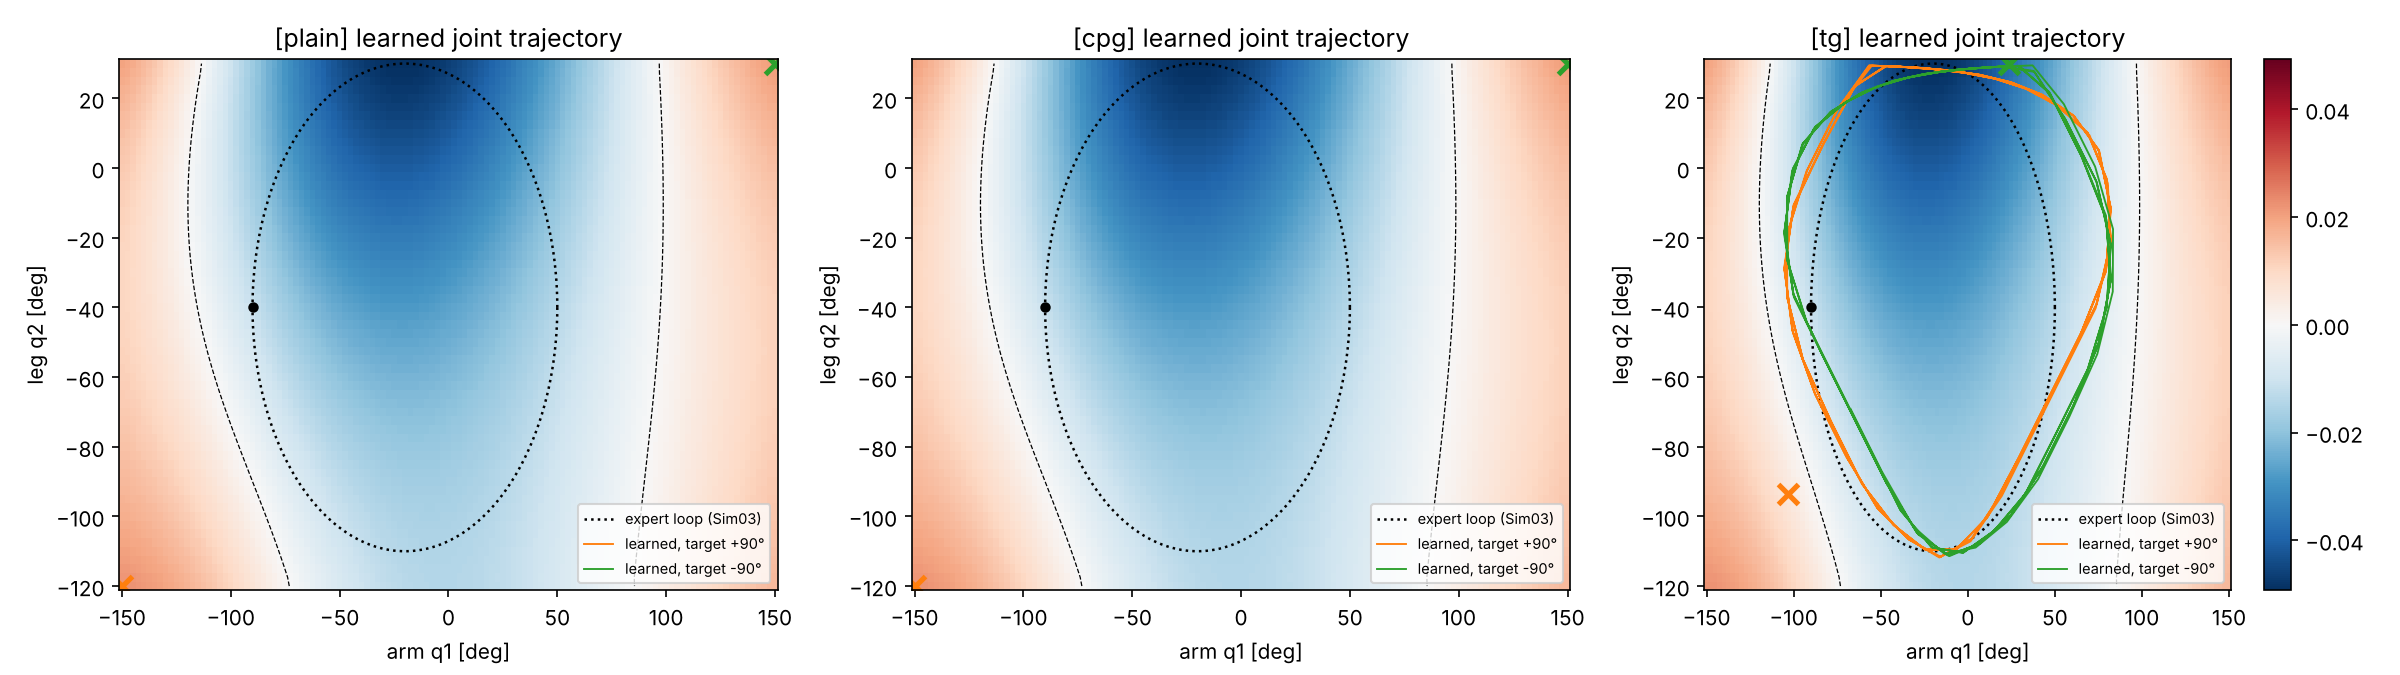
\includegraphics[width=0.86\textwidth]{figs/learn_top.png}
\caption{学習した関節の軌道（色は接続の曲率 $F$）。plain と cpg は手足を可動域の端まで振って止まる局所解（×印）に収束する。
振動子の構造を持つ tg は、曲率が負の領域をほぼ埋めるループを見つけた。点線は人手で設計した最適円ループ。}\label{fig:learn}
\end{figure*}

\textbf{結果}（表~\ref{tab:learn}、図~\ref{fig:learn}）：plain と cpg は、手足を可動域の端まで振って止まる局所解に収束した。
tg は数十イテレーションで解を見つけ、1 周 $+9.34^\circ$ のループを学習した。これは人手で設計した最適円（$+6.70^\circ$）を上回り、可動域内の理論上界（$+9.57^\circ$）の 98\% に達する。
回す向きも曲率の符号と整合し、最後に「揺れの少ない位相で止まる」ことまで覚えて、終端誤差は expert より 1 桁以上小さかった。

\textbf{なぜ構造なしでは失敗するのか}：1 回の動きの効果（可逆な首振り $-\bm\Gamma\cdot\Delta\bm q$）は振幅の 1 次だが、ループの正味の回転（曲率 × 囲んだ面積）は振幅の 2 次（$\propto A_1A_2$）である。
静止に近い方策から探索を始めると、ループを大きくする方向の勾配はほぼ 0 になり、1 次の効果である「端まで振る」が先に最適化される。
これはハイパーパラメータの問題ではなく、課題の物理構造に由来する。周期信号を観測に足すだけ（cpg）では足りず、「ループを描く」という\textbf{形}を方策の構造として与えることが成否を分けた。
plain と cpg の誤差が 3 つの目標で完全に一致するのは、両者が同じ「端まで振る」解に収束したことの表れである。

同じ現象は地上でも現れた（段階 6、第~\ref{sec:legground} 節）。MuJoCo \cite{todorov2012} を評価関数として直接使い、荷物運びの腰と肘の動きを Nelder--Mead 法で最適化したところ、
最初から短い動作時間で探すとどの係数でも転倒して評価が平らになり、探索が進まなかった。
時間を少しずつ短くする継続法で、荷物運びの時間は 65\% 短縮し、「反ってから前に傾く」という人が重い物を持つときの動き（腰の戦略）が再発見された。
\textbf{評価が平らになる領域を、物理の構造から予測し、避ける設計}が、安価なシミュレーションで事前に検討できる。


\section{課題 2：モデル誤差と、学習・最適制御の分担}\label{sec:robust}

\textbf{設定}：18 m 級の機体で、スラスタと AMBAC を併用して 90° の旋回を 60 s で行う。
制御器は周回平均の「平均化モデル」しか知らず、評価には周回内の揺れを含む「位相モデル」を用いる（モデル誤差）。
さらにループ形状の効き（$\times0.7$〜$1.3$）、慣性（$\times0.9$〜$1.1$）、一定の外乱トルクをランダムに変えた 100 例で比べた。
学習方策は観測（平均姿勢の誤差、角運動量、残り時間、ループの位相）からスラスタのトルクとループの周波数を出す MLP で、同じランダムな条件で学習した（ドメインランダム化 \cite{peng2018}）。

\begin{table}[t]\centering\small
\caption{モデル誤差・外乱がある 100 例での比較}\label{tab:robust}
\setlength{\tabcolsep}{4pt}\begin{tabular}{lccc}\toprule
制御器 & 終端誤差 & 残留角速度 & 推進剤 \\
 & 平均（95\%） & [°/s] & [kg] \\\midrule
開ループ最適制御 & 30.5°（68.8°） & 0.90 & \textbf{1.97} \\
MPC & 14.6°（23.3°） & 0.030 & 5.41 \\
MPC＋揺れ補償 & 0.19°（0.69°） & 0.031 & 5.56 \\
学習方策 & \textbf{0.09°（0.10°）} & \textbf{0.002} & 4.92 \\\bottomrule
\end{tabular}
\vspace{1pt}\par\footnotesize 参考：公称モデルでのスラスタのみの最適値は 3.62 kg。
\end{table}

\textbf{結果}（表~\ref{tab:robust}）：線形計画で解いた開ループの最適制御は、推進剤は最小だが、終端誤差が 30° に達した。
平均化モデルの予測自体は正確（平均姿勢 89.6° 対予測 90.0°）で、誤差の原因は止まった位相での揺れだった。
人手で揺れの補償を加えた MPC は誤差 0.19° まで改善したが、学習方策は\textbf{観測に位相を入れただけで}同じことを自力で獲得し、誤差 0.09°、残留回転は MPC の 1/10 だった。
実行時の計算も行列積だけで済む（100 例で 0.1 s 対 LP の再計画で 15〜40 s）。

一方、学習方策の推進剤は、スラスタだけの最適値より多かった。
スラスタで角運動量を一度入れると、止めるときに同じ量の逆噴射が必ず要るため、\textbf{AMBAC が推進剤を節約できるのは「最初にどれだけ噴くか」を決める段階だけ}である。
報酬が終端でしか与えられない学習では、この最初の判断の価値を割り当てにくく（信用割り当ての問題）、学習方策は AMBAC で得をする余地を自ら消していた。

\textbf{示唆}：保存量（角運動量）の収支のように、最適性が明示的な構造で決まる部分は最適制御で計画し、
モデル誤差・外乱・速い揺れの補正は学習で担う、という分担（残差学習 \cite{johannink2019}）が自然である。
第~\ref{sec:learn} 節と合わせると、\textbf{「形」（ループ）は方策の構造として与え、「保存量」は計画で扱う}という、物理の知識と学習の分担の指針が得られる。


\section{シミュレーション場：方法}\label{sec:field}

ここからが、現在進めている第 2 段階である。
PC 上に、障害物のない「試験場」と、段差・坂・低摩擦面・低重力などを置ける「ステージ」を用意し、物理エンジン MuJoCo（CPU のみ）で機体を動かす。
目的は、\textbf{組み合わせた形で、要求した動きを実現できるか}を、校正値と制御を含めて確かめることである。進め方は次の 4 つである。

\begin{enumerate}\setlength{\itemsep}{0pt}
\item \textbf{3 層の照合}：第 1 段階の Python の基準モデル（答えが分かっている）と MuJoCo を照合してから、MuJoCo でしかできない試験に進む。将来の実機を 3 層目とする（第~\ref{sec:bangai} 節）。
\item \textbf{部品表から機体を組み立てる}（アセンブル）：台車・腰・肩（1〜3 軸）・肘・履帯・ばね・円盤などを JSON の部品として組み合わせる。
\item \textbf{段階的に組み込む}：基準の試験に仕組みを 1 つずつ足し、同じ物差しで比べる。
\item \textbf{目で確かめる}：数値とグラフに加えて、動画で動きを見る。履板の食い込み、床を突き抜けた腕、電源を切った後に動く腕は、動画で見つけた。
\end{enumerate}

\textbf{シミュレータ自体の照合}：基準モデルと MuJoCo を同じ関節の動きで比べた。
腕 1 本の往復で $-16.0356^\circ$ 対 $-16.0356^\circ$、腕＋脚のループ 1 周で $+2.963^\circ$ 対 $+2.970^\circ$ と一致し、角運動量の保存は $10^{-6}$ 程度だった（この照合は積分法 RK4 による）。
ゲーム用の物理エンジンは安定化のための減衰などで角運動量が厳密には保存されないことがあり、1 周数度の幾何学的位相は埋もれうる。
\textbf{答えの分かっている試験に合格させること自体が、シミュレータの校正}になる。
ただし第~\ref{sec:calib} 節で見るように、この照合に合格した後でも、部品表から組み立てた機体の既定の積分法（implicitfast、1 次）が、校正の試験では系統誤差の源になった。
照合は「どの積分法・時間刻みで」合格したかまで含めて記録する必要がある。

\begin{figure*}[t]\centering
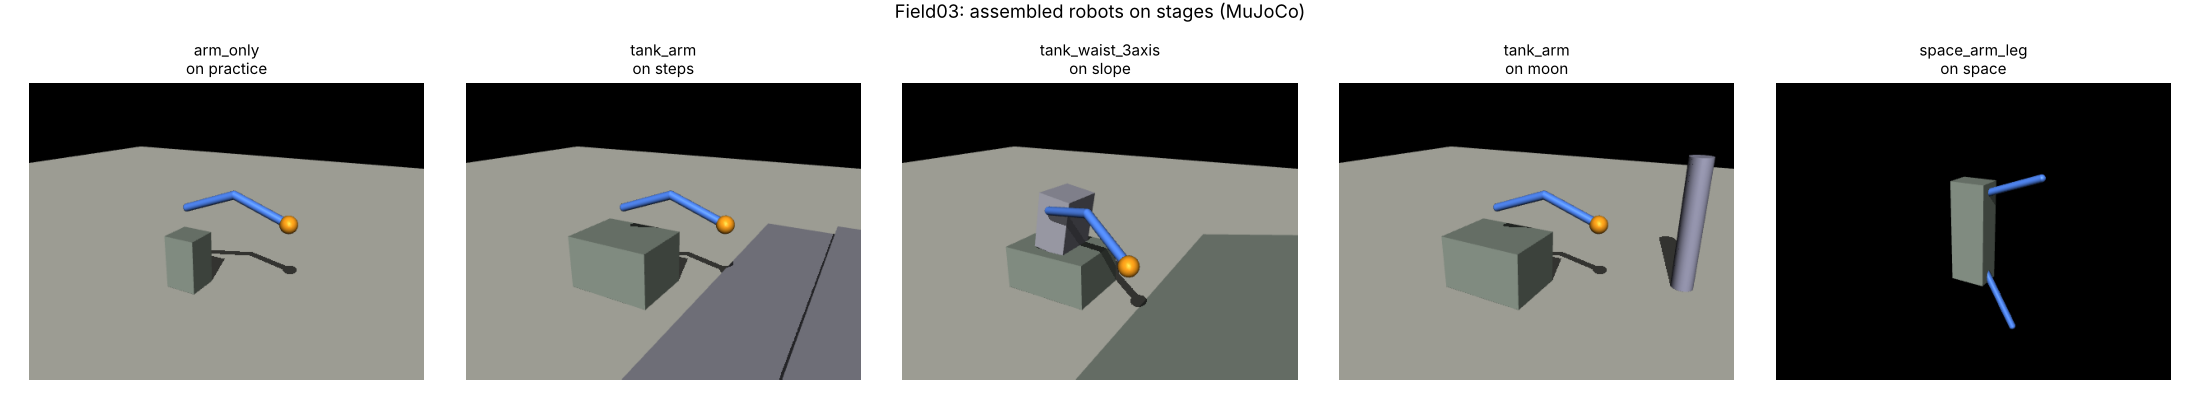
\includegraphics[width=0.92\textwidth]{field/field03_gallery.png}
\caption{部品表（JSON）から組み立てた機体の例（段階 3）。台車・腰・肩・肘・履帯などの部品を組み合わせ、手作りのモデルと同じ結果になることを確かめてから、ステージでの試験に使った。}\label{fig:gallery}
\end{figure*}


\section{シミュレーション場：全体の結果}\label{sec:fieldres}

\begin{table*}[t]\centering\small
\caption{シミュレーション場の段階ごとの成果}\label{tab:stages}
\setlength{\tabcolsep}{4pt}
\begin{tabular}{clp{0.62\textwidth}}\toprule
段階 & 内容 & 主な結果 \\\midrule
1 & 宇宙の試験場 & 基準モデル（腕の往復 $-16.04^\circ$、ループ 1 周 $+2.98^\circ$）と一致。シミュレータの妥当性を確認 \\
2 & 地上の試験場 & 転倒の始まりが基準モデルと一致。旋回で台車が浮く条件（第 1 段階の前提が崩れる場合）を発見 \\
3 & アセンブル & 部品表から機体を組み立て、手作りのモデルと一致 \\
4 & 仮想の実機で校正 & 答えを隠した機体の質量・慣性を推定。誤差の評価と kinematic fit は第~\ref{sec:calib} 節 \\
5 & 性能表・校正データ & 重力だけが違うステージではフルード則が 1\% の精度で成立、氷では外れる。CSV・JSON・Excel を出力 \\
6 & 腰の戦略の最適化 & 荷物運びを最大 65\% 短縮。「反ってから前に傾く」動きを再発見。トルクは 3 倍に \\
7 & モーターの定格 & 荷物を支えるトルク（地球 130・月 22 N·m）が実現の境目 \\
8・10 & 段差・坂（履帯） & 坂は摩擦の限界（31°）どおり。段差は長い履帯で 2 倍（0.15 → 0.30 m）。短い機体は後ろに転倒 \\
9 & 二本脚と戦車型 & 二本脚は腰なしでは荷物を運べない。腰ありでも戦車型より約 3 割遅い \\
11 & 2 本の履帯の旋回 & スキッドステアの基準モデルと 0〜11\% で一致。長い履帯は旋回に 1.6 倍の力。荷重分布を一様と仮定すると 3 割ずれる \\
12 & 腕の振りと向き & 腕の非対称な往復で車体を回せる（摩擦の非対称性による地上版 AMBAC） \\
13 & 腕の反作用への対策 & 車体が回るのは腕を「止めるとき」。しなり（ばね）は逆効果、逆回転するおもりは有効 \\
14 & 止め方・流体ブレーキ & トルクを境目より下に抑えて止めると、車体を回さずに 1.2〜1.35 s で振れる。流体の種類で得意な場面が逆 \\
15 & 機能を分けた組み合わせ & 動かす＝モーター、止める・保持する＝MR ブレーキで 1.18 s、行き過ぎ 0.2°、電源なしでも保持 \\
16 & 繰り返しの発熱と劣化 & 先に限界に達するのはモーター。MR で止めると続けられる頻度が 2 倍。寿命は約 150 万回 \\
17 & 3 軸の肩＋肘 & モーター＋MR が、車体を乱さない方式で最速。電源を切っても腕が落ちない（2 mm） \\
18 & 宇宙の脚の円錐 & 式と $10^{-5}$° で一致。可動域と脚どうしの干渉で 48.2° → 32.8°/周 \\
19 & 足裏の摩擦と足首 & 滑りの境目は足のねじれで決まる（必要な摩擦 0.88、予測 0.16） \\
20 & 二本脚の段差 & 上体の前傾で 0.13 → 0.33 m（Sim10 の式の 55〜70\%）。$s=2$ では踏み出せない \\
21〜26 & 歩行 & ZMP の計画で歩ける。腕の振りで足のねじれが消える。安定化と踏み出し。実機で測れる量からの重心の推定と脚のオドメトリ（第~\ref{sec:walk} 節） \\\bottomrule
\end{tabular}
\end{table*}

段階ごとの成果を表~\ref{tab:stages} にまとめる。上半身（腕・肩）の段階 12〜17 は第 II 部（第~\ref{sec:upperground} 節）、下半身（腰・脚・足回り）の段階 6・8〜10・18〜26 は第 III 部（第~\ref{sec:legground}・\ref{sec:steps}・\ref{sec:walk} 節）、段階 4 の校正は第 IV 部（第~\ref{sec:calib} 節）で詳しく述べる。本節では、部位をまたいで得られた結果をまとめる。

\textbf{性能を左右する校正値}：組み立てた機体の試験から、表~\ref{tab:calibvals} の量が性能を大きく左右することが分かった。
これらは、\textbf{モデルに含めた誤差源の中で}、実機で何を先に測るべきかの候補を与える。
重力だけが違うステージでは荷物運びの最短時間がフルード則（$\propto\sqrt{\text{大きさ}/g}$）で 1\% の精度で移せたが、氷では外れ（予測 1.35 s 対 2.22 s）、制約が転倒から滑りに変わった。摩擦は重力のスケーリングとは別の校正値である。

\begin{table}[t]\centering\small
\caption{性能を左右すると分かった校正値}\label{tab:calibvals}
\setlength{\tabcolsep}{3pt}
\begin{tabular}{p{0.42\linewidth}p{0.38\linewidth}c}\toprule
校正値 & 何を決めるか & 段階 \\\midrule
質量・慣性（腕・脚・胴体） & AMBAC の効き & 4 \\
足元の摩擦の境目と荷重移動による変化 & 腕の作業で車体が乱れるか & 12〜14 \\
接地の荷重分布 & 旋回の速さ（一様の仮定で 3 割ずれる） & 11 \\
関節の慣性（姿勢で変わる） & 止める計算 & 17 \\
サーボの遅れ（ゲイン） & 軌道の崩れ、急ブレーキ & 13 \\
摩擦（重力とは別） & 氷でのフルード則の破れ & 5 \\
モーターの銅損・熱抵抗、MR の温度係数・寿命 & 続けて動かせる頻度、保守の周期 & 7・16 \\\bottomrule
\end{tabular}
\end{table}

\textbf{シミュレーション場を作るうえでの教訓}：
MuJoCo は計算が発散すると状態を初期化するため、発散が「止まった」結果に紛れる。走行の試験では発散を検出して記録するようにした。
また、腕の動き（秒）と温度（分〜時間）のように時間の桁が違う現象は、前者を MuJoCo、後者を熱の簡単なモデルで扱い、組み合わせた。


\part{上半身の詳細：肩と腕}

第 I 部では、腕と脚を平面の 2 つの関節として扱った。第 II 部では、上半身（肩と腕）を 3 次元で扱い、
宇宙での AMBAC（第~\ref{sec:upper3d} 節）、地上での腕の反作用と止め方（第~\ref{sec:upperground} 節）を詳しく述べる。
上半身は、第 1 段階の Sim07・Sim08 と、シミュレーション場の段階 12〜17 で、MuJoCo まで含めて最も多く検証した部位である。

\section{3 次元の肩：円錐の AMBAC とひねりの幾何学的位相}\label{sec:upper3d}

\textbf{3 次元の AMBAC}（Sim07）：腕の向きを肩を原点とする球面座標（方位角 $\psi$、仰角 $\alpha$）で表し、胴体の姿勢は回転行列で積分した（オイラー角は特異点を持つため使わない）。
人間大のモデルで腕に円錐を描かせると、1 周あたりの胴体の回転は半頂角 10°・30°・45°・70° で 0.65°・5.7°・12.4°・25.4° と、半頂角とともに急に増えた。
円錐の軸の向きでも変わり（半頂角 45°）、前方 12.4°、右横 11.1°、前上方 45° で 39.7°、真上（方位角を 1 周させる旋回）で 58.0° だった。
胴体の回転軸は円錐の軸と 8〜31° ずれる。3 次元の回転は順序で結果が変わり、ヨー → ピッチとピッチ → ヨーでは最終姿勢が 29.4° 違った。
球面座標には極（ジンバルロック）があり、ループが極に 0.3° まで近づくと方位角の速度は 300 rad/s に発散する。\textbf{座標の特異点を作業範囲の外に置く}ことが、肩の設計の要件になる。

\textbf{肩のひねりも幾何学的位相である}（Sim08）：腕を「下 → 前 → 横 → 下」と動かして元の向きに戻すと、一度もひねっていないのに上腕が長軸まわりに 90° ひねられる（コッドマンのパラドックス \cite{codman1934}）。
ひねりの角速度を 0 に保って動かすと、ループ 1 周後のひねりは、腕の向きが単位球面上で囲んだ立体角に等しい（ガウス・ボンネの定理）。
計算でも、古典的な動作で 90.00°、半頂角 20°・45°・90° の円錐で 21.71°・105.44°・360.00° と、立体角と一致した。
AMBAC（関節角の空間のループ → 胴体の回転、接続の曲率の面積分）と肩（球面上のループ → 上腕のひねり、球面の曲率の面積分）は、同じ数学で書ける。
2 軸ジンバルの肩ではこのパラドックスは起きないが、代わりにひねりを独立に選べない。

\textbf{腕組みに必要な肩の機構}（Sim08）：右手を左の上腕に置く腕組みを、腕（円柱）が胸郭（楕円柱）に食い込まない条件で解いた（表~\ref{tab:armcross}）。
2 軸ジンバルの肩は、胸の厚さによらず届かない（手の誤差 24〜26 cm）。前腕の曲がる面が上腕と同じ鉛直面に固定されるためである。
球関節だけでは、腕組みに人の限界（内旋 70〜90°）ぎりぎりかそれ以上の内旋が要り、胸が厚い（装甲）と 110° に達する。
肩甲骨・鎖骨（上肢帯）で肩関節の中心を前に出すと、必要な内旋は 15〜35° 減って人の範囲に収まる。\textbf{人が腕を組めるのは、肩甲骨が動くから}である。

\begin{table}[t]\centering\small
\caption{腕組みに最低限必要な内旋量（Sim08）}\label{tab:armcross}
\setlength{\tabcolsep}{2pt}
\begin{tabular}{lcc}\toprule
胸の奥行 & 球関節のみ & 球関節＋上肢帯（前方突出） \\\midrule
0.18 m（細身） & 86° & 71°（12°） \\
0.22 m（標準） & 93° & 73°（16°） \\
0.26 m（厚い胸） & \textbf{110°} & 75°（20°） \\\bottomrule
\end{tabular}
\vspace{1pt}\par\footnotesize 人の内旋の可動域はおよそ 70〜90°（姿勢と測り方に依存）。2 軸ジンバルは不可。
\end{table}

\begin{figure*}[t]\centering
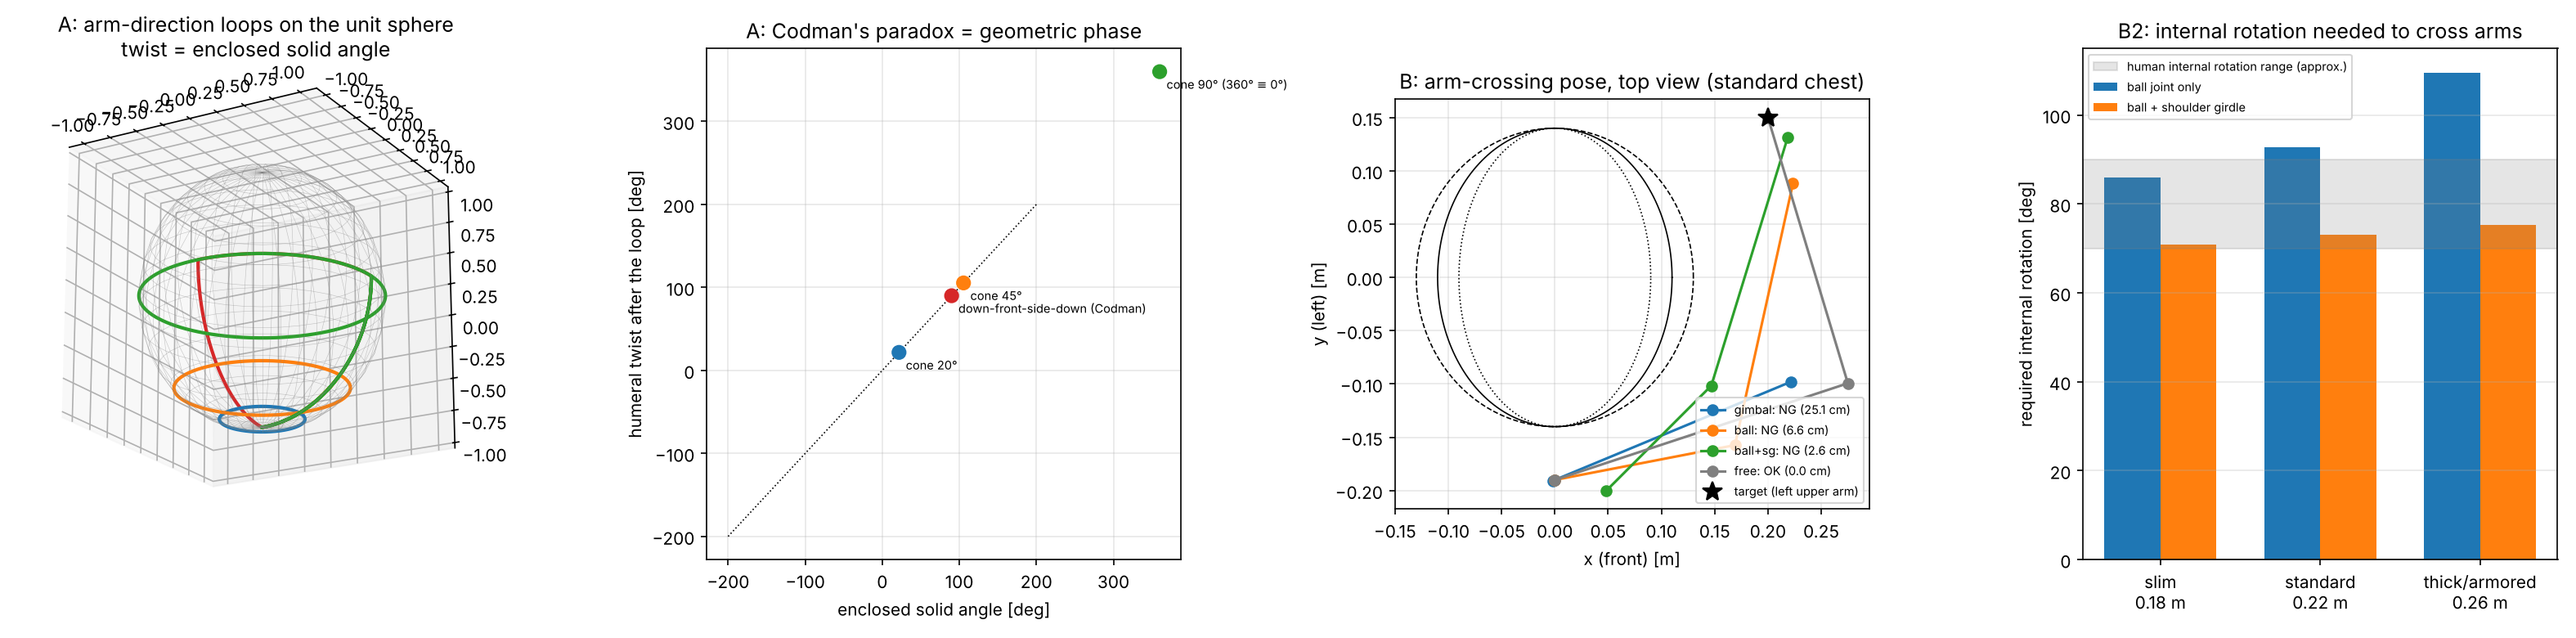
\includegraphics[width=0.94\textwidth]{sim08_shoulder.png}
\caption{肩の幾何学的位相と腕組み（Sim08）。ひねらずに動かした腕のひねりは、腕の向きが単位球面上で囲んだ立体角に等しい（コッドマンのパラドックス）。腕組みは、上肢帯で肩の付け根を前に出すと人の可動域で可能になる。}\label{fig:shoulder}
\end{figure*}

\textbf{フィジカル AI への示唆}：モーションキャプチャーで人の動きをロボットに移すとき、ひねりの扱いを誤ると、同じ腕の向きでも手のひらの向きが変わる。
ひねりは腕の向きの\textbf{経路}で決まるため、終端の姿勢だけを目標にする学習や模倣では制御できない。
第~\ref{sec:learn} 節の「ループの形を構造として与える」と同じく、\textbf{ひねり（3 自由度目）を明示的に計画・計測すること}が、人間らしい動きを再現する機械の要件になる。


\section{地上の腕：反作用・止め方・機能の分担}\label{sec:upperground}

地上では、腕の反作用は機体の回転ではなく、足元（履帯・足裏）への力として現れる。
戦車型の台車に 3 次元の腕を載せた機体（Sim07 Part B、シミュレーション場の段階 12〜17）で、腕の作業が車体を乱す仕組みと、その抑え方を調べた。

\textbf{腕の向きで持てる荷物が変わる}（Sim07）：転倒しない静的な最大荷重は、前・斜め前・後で 41.5〜42.2 kg だが、横では 24.3 kg と 4 割落ちた。台車の支持範囲が横に狭いためである。
荷物 10 kg を前から後ろへ水平に 180° 回す動作は、水平のままでは 1.83 s だが、途中で腕を下げると 1.01 s、仰角と旋回のタイミングを最適化すると 0.88 s（52\% 短縮、月でも 54\%）になった。

\textbf{地上の反作用と足元の摩擦の境目}（段階 12〜13）：
宇宙では腕の反作用はすべて機体の回転になるが、地上では、\textbf{足元の摩擦が車体を回し始めるトルク（この機体で約 260 N·m）までは、反作用を摩擦が吸収する}。
境目を超えた分だけが、車体の回転や滑りとして現れる。車体を乱すのは主に腕を\textbf{止めるとき}で、位置サーボの遅れ（最大 17°）が急ブレーキを生み、この境目を超えさせていた（図~\ref{fig:reaction}）。
反作用の山の高さだけでなく、境目を超えている時間（力積）が効くため、しなり（ばね）は山を下げても境目より下まで下げられなければ逆効果だった。逆回転するおもりは有効だが、横倒しに注意が要る（0.6 s で横倒しになった例は第~\ref{sec:fail} 節の索引）。
一方で、摩擦の非対称性を使えば、腕を「速く振ってゆっくり戻す」往復で車体の向きを変えられる。宇宙の AMBAC（幾何学的位相）とは別の仕組みの、\textbf{地上版の AMBAC} である。駆動力の足りない旋回を腕で助けることもできた。

\begin{figure*}[t]\centering
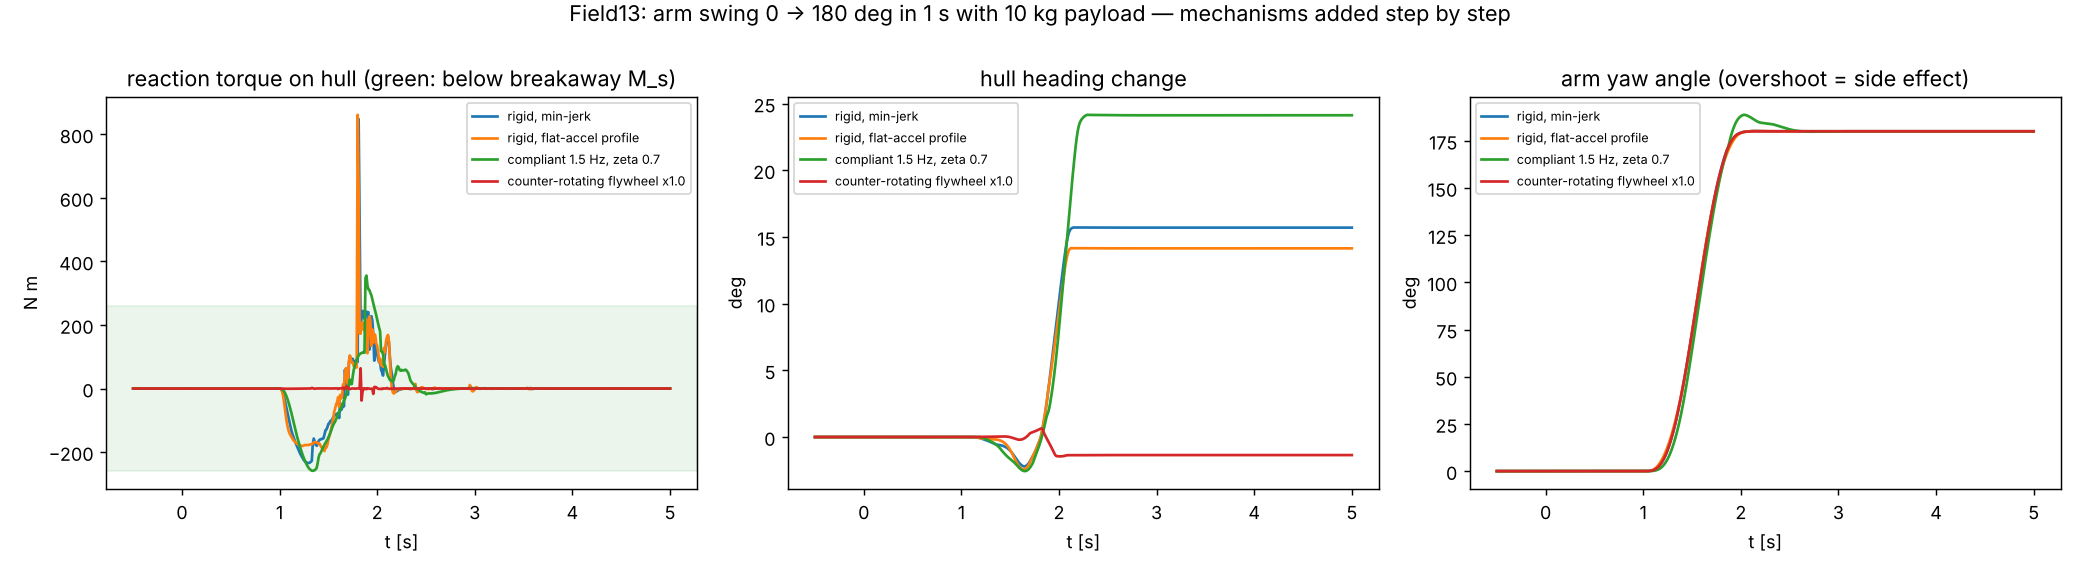
\includegraphics[width=0.92\textwidth]{field/field13_reaction.png}
\caption{腕の反作用と車体の回転（段階 13）。車体が回るのは、腕を止めるときの反作用が足元の摩擦の境目を超えた区間で、位置サーボの遅れがその急ブレーキを生む。しなり（ばね）は山を下げるが、境目を超える時間（力積）を減らせず逆効果になる。}\label{fig:reaction}
\end{figure*}

\textbf{止め方を変える・機能を分ける}（段階 14〜17）：止め方を変える（トルクを境目より下に抑えて一定に止める）だけで、追加の部品なしに車体を乱さず 1.2〜1.35 s で振れた。
流体ブレーキは種類で得意な場面が逆になり、ダイラタントは速い動きを止める、擬塑性はゆっくりした力に耐える、チキソトロピーは休むと固まる、MR（磁気粘性）は止める・保持する強さを制御できる。
さらに、動かすのはモーター、止める・保持するのは MR 流体のブレーキ、と機能ごとに部品を分けて上の制御で使い分けると、速さ・精度・省エネ・電源なしの保持が同時に向上した（段階 15：1.18 s、行き過ぎ 0.2°）。
3 軸の肩と肘の腕全体（段階 17、表~\ref{tab:arm3d}）でも同じ結論が成り立ち、電源を切ったときの安全で大きな差が出た。
人の体の筋肉（動かす）・腱（しなる）・靭帯や関節の摩擦（保持する）と同じ考え方である。
MR は熱で効きが落ち、使うほど劣化するが、劣化は熱に変えたエネルギーの総量（LDE）で予測でき（寿命は約 150 万回）、MR で止めるとモーターの発熱が減って続けて動かせる頻度が 2 倍になった（段階 16。温度係数と寿命は製品のデータで要確認）。

\begin{table}[t]\centering\footnotesize
\caption{3 軸の肩＋肘の腕全体で、荷物を 2 区間動かす（段階 17）}\label{tab:arm3d}
\setlength{\tabcolsep}{1.4pt}
\begin{tabular}{lcccl}\toprule
方式 & 時間 & 車体の向き & 銅損 & 電源を切ったとき \\\midrule
位置サーボ・速い & 2.14 s & $-7.7^\circ$ & 2167 J & 1.0 m 落ちる \\
位置サーボ・遅い & 3.98 s & $0.0^\circ$ & 1566 J & 1.0 m 落ちる \\
トルク制御 & 2.93 s & $0.1^\circ$ & 2867 J & 落ちて車体が倒れる \\
\textbf{モーター＋MR} & \textbf{2.81 s} & $0.4^\circ$ & 2153 J & \textbf{2 mm 下がる} \\\bottomrule
\end{tabular}
\end{table}

\begin{figure*}[t]\centering
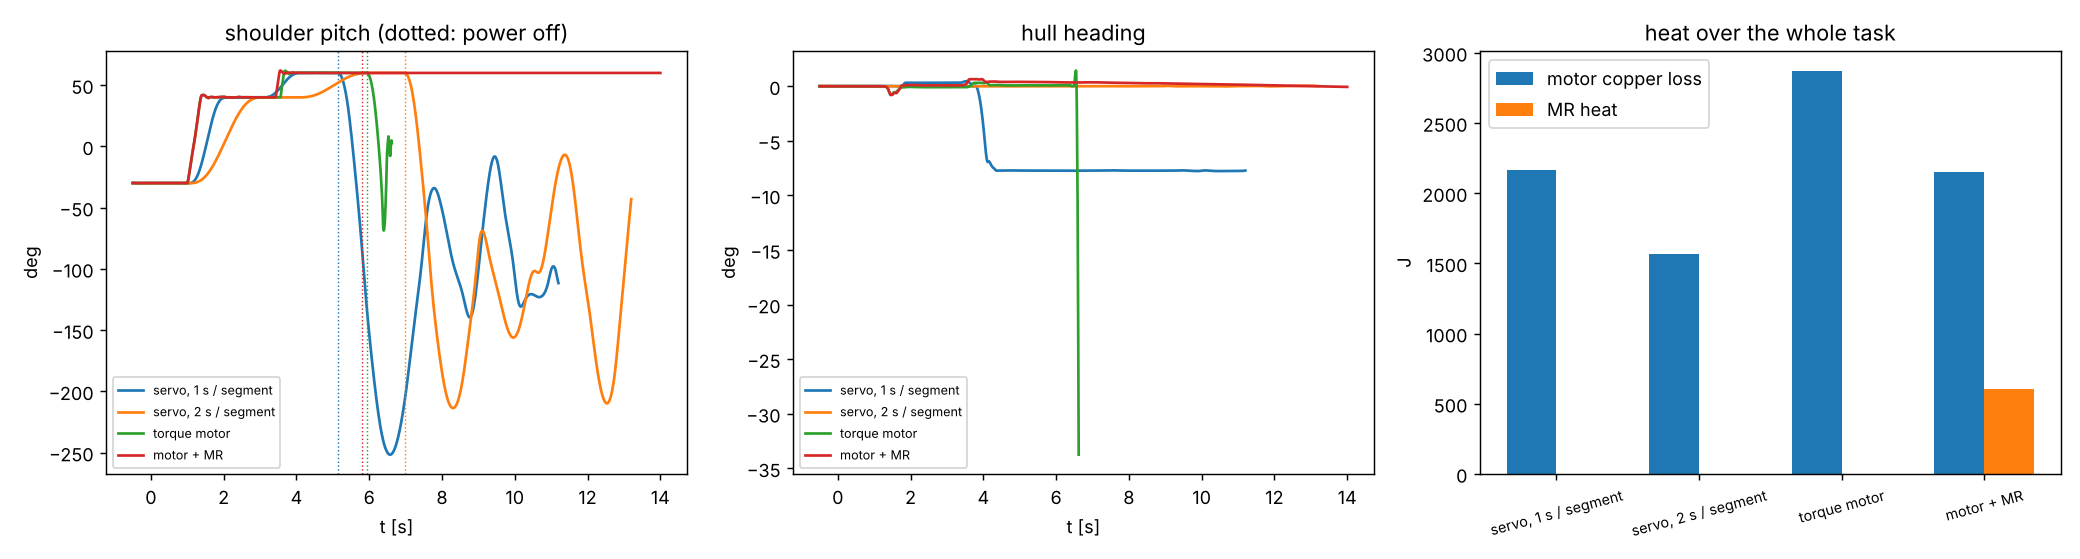
\includegraphics[width=0.94\textwidth]{field/field17_arm3d.png}
\caption{3 軸の肩＋肘の腕全体の比較（段階 17）。モーターで動かし MR で止める・保持する方式が、車体を乱さない方式の中で最速で、電源を切っても腕が落ちない。}\label{fig:arm3d}
\end{figure*}

\textbf{上半身で残っている課題}：
腕の各関節の部品（モーター・MR）の重さと大きさは機体の質量に含めていない。MR の保持の硬さは仮定である。
関節の慣性は姿勢で大きく変わるため、止める計算はその場の慣性で計算し直す必要がある。
肩のモデルでは胸郭を楕円柱、腕を円柱で近似し、可動域は姿勢によらない上限で単純化した。左右の腕どうしの干渉、肩甲骨を含む腕組みの\textbf{動作}（姿勢だけでなく経路）、速く振ったときの横の転倒は扱っていない。
腕の 3 次元の AMBAC（円錐）は式のモデルだけで、MuJoCo での照合は平面のループまでである。

\part{下半身の詳細：脚と腰}

第 III 部では、下半身（脚と腰）を、宇宙（第~\ref{sec:legspace} 節）、地上での立つこと・荷物を運ぶこと（第~\ref{sec:legground} 節）、段差（第~\ref{sec:steps} 節）、歩行（第~\ref{sec:walk} 節）の 4 つの場面で扱う。
第 3 版までは第 1 段階の式のモデル（Sim09・Sim10）が中心で、MuJoCo での検証は脚を固定した二本脚（段階 9）と腰の最適化（段階 6）だけだった。
第 4 版では、式のモデルの結論を MuJoCo で 1 つずつ確かめ（段階 18〜20）、歩行（段階 21〜24）を加えた。どの段階でも、誤差を計算・系統・入力に分けて評価し、うまくいかなかったことを F21〜F45 として残した（第~\ref{sec:fail} 節）。

\section{宇宙の脚：最も効く「重い肢」}\label{sec:legspace}

「足なんて飾りです」という有名な台詞がある。コストだけを見れば、脚の代わりに台車にした方が安い。物理的に、脚は飾りなのか。
まず宇宙で、総質量 76 kg をそろえて、1 周あたりに稼げる回転の上限（関節の可動域の中で、同じ符号の曲率の領域をすべて囲んだ場合）を比べた（表~\ref{tab:legspace}）。

\begin{table}[t]\centering\small
\caption{宇宙での脚の効き（Sim09、総質量 76 kg）}\label{tab:legspace}
\footnotesize\setlength{\tabcolsep}{2pt}
\begin{tabular}{lcc}\toprule
平面：構成 & 1 周の上限 & 90° の周回 \\\midrule
腕＋脚（人間型） & 9.57° & 10 \\
腕＋腕（脚の質量は胴体へ） & 5.71° & 16 \\
腕だけ & 0° & 不可能 \\
腕＋重い脚（脚 2 倍） & \textbf{12.87°} & 7 \\\midrule
3 次元：円錐（前下方 30° の軸） & \multicolumn{2}{c}{1 周の胴体の回転} \\\midrule
腕（肩）、半頂角 30° & \multicolumn{2}{c}{24.8°} \\
\textbf{脚（股関節）、半頂角 30°} & \multicolumn{2}{c}{\textbf{48.2°}（腕の 1.9 倍）} \\
脚（股関節）、半頂角 45° & \multicolumn{2}{c}{96.8°} \\\bottomrule
\end{tabular}
\end{table}

脚を外すと姿勢を変える能力は半分近くまで落ち、腕 1 本だけでは平面では不可能になる（関節 1 つでは往復で元に戻る。第~\ref{sec:ambac} 節）。
3 次元でも、股関節の可動域は肩より狭いが、脚は腕の約 3 倍重く長いので、同じ円錐の動きで胴体を 1.9 倍回せる。
脚に質量（推進剤のタンクや装甲）を集めるほど、AMBAC は強くなる。\textbf{宇宙では、脚は飾りではなく、AMBAC で最も効く肢である。}

第 I 部の学習（第~\ref{sec:learn} 節）と制御（第~\ref{sec:robust} 節）、MuJoCo との照合（第~\ref{sec:field} 節、ループ 1 周 $+2.963^\circ$ 対 $+2.970^\circ$）、第 IV 部の校正（第~\ref{sec:calib} 節）は、すべてこの腕＋脚のモデルで行った。
脚の質量は、校正で推定する 3 つのパラメータの 1 つであり、正味の回転だけでは推定できない（F1）ことも、脚の寄与の大きさと関係する。

\textbf{MuJoCo での照合と、形を入れて初めて分かる制約}（段階 18、図~\ref{fig:lower1}(a)）：脚の円錐を MuJoCo で動かすと、式と $10^{-5}$°（命令ではなく MuJoCo が実際にたどった経路を式に入れた比較）で一致した。
最初の比較の $-1.13\%$ の差はサーボの遅れ（追従誤差 4.3°）で円錐が縮んでいたためで（F22）、脚の太さの効果も、自在継手が脚を軸まわりにねじる分を入れて初めて式と合った（F23）。
ところが、関節の可動域ともう 1 本の脚の形を入れると、\textbf{Sim09 の円錐（内転 35°）は 1 周の 20\% でもう 1 本の脚にぶつかる}（すき間 $-8.2$ cm、F21）。
可動域の中で脚どうしが当たらない組の最大は 1 周 32.80°（MuJoCo 32.76°）で、式の 48.2° の 68\%。それでも腕の円錐の 1.3 倍あり、「宇宙では脚が最も効く肢」という結論は残る。
式のモデルは手足を点質量の線にまとめていたため、形どうしの干渉を調べようがなかった。\textbf{2 層目の照合は、数値の一致だけでなく、1 層目が前提にした動きが実現できるかを確かめる}。

\section{地上の脚：立つことと荷物を運ぶこと}\label{sec:legground}

\textbf{二本脚は静的にはバランスが悪い}（Sim09 Part B）：Sim06 と同じ荷物運び（10 kg を前方の低い位置から後方の高い位置へ）を、同じ腕・同じ総質量 97 kg の戦車型（接地長 0.8 m）と二本脚（足裏 0.25 m、重心が高い）で比べた。
腕だけを最適化すると、戦車型は 0.98 s で運べるが、二本脚は\textbf{静止していても転倒する}と判定された。足裏の支持範囲（±0.125 m）が狭く、荷物を前に持つと ZMP がつま先を越える。
上体を前後に傾ける（股関節で上体を動かす）と、二本脚でも 0.69 s で運べた。荷物を前に持つときは後ろに反り（$-40^\circ$）、後ろに置くときは前に傾く（$+28^\circ$）。
重い上体（56 kg）を動かして腕の反作用を打ち消す\textbf{地上版の AMBAC} で、人の姿勢制御でいう腰の戦略 \cite{horak1986} である。ただし、上体を傾けられるなら戦車型の方がさらに速い（0.64 s）。

\textbf{腰の戦略を MuJoCo で再発見する}（段階 6）：戦車型の台車に前後に傾く腰と 3 軸の肩を載せた機体（97 kg）で、MuJoCo を評価関数として直接使い、腰と肘の動きを Nelder--Mead 法で最適化した（物理の式を使わない探索）。
腰の補正は肘の補正より効き（練習場で 60\% 対 42\% の短縮）、両方で 65\%（1.41 → 0.50 s、月でも 62\%）短くなった。
見つかった腰の動きは「最初に後ろへ反り、荷物を後ろに回すにつれて前へ傾く」で、Sim09 の最適解と同じ型だった。
最初から短い時間で探すと評価が平らになり探索が進まず、継続法で解決した（第~\ref{sec:learn} 節）。速くなる代わりに必要なトルクは 318 → 1102 N·m に増える。

\textbf{二本脚と戦車型を MuJoCo で比べる}（段階 9、表~\ref{tab:biped}）：Sim09 と同じ寸法の二本脚（脚 24 kg・足裏 0.25 m、股関節 0.95 m で前後に傾く上体 56 kg）を組み立てた。
脚は固定し、足首は十分に強いと仮定した（支持範囲は足裏の大きさで決まる）。
二本脚は腰を 0° から始めるとどの補正でも転倒したため、腕の各姿勢で全体の重心が足裏の中央に来る腰の角度（静的なつり合い）を先に計算し、それを出発点にした。

\begin{table}[t]\centering\small
\caption{荷物運びの安全な最短時間（段階 9、傾き 1° 未満・ずれ 5 mm 未満）}\label{tab:biped}
\setlength{\tabcolsep}{3pt}
\begin{tabular}{lcccc}\toprule
 & \multicolumn{2}{c}{練習場} & \multicolumn{2}{c}{月} \\
腰・肘の使い方 & 二本脚 & 戦車型 & 二本脚 & 戦車型 \\\midrule
腰を使わない & \textbf{不可} & 1.41 s & \textbf{不可} & 3.47 s \\
腰：静的なつり合い & 0.94 s & --- & 2.16 s & --- \\
腰：最適化 & 0.74 s & 0.57 s & 1.98 s & 1.51 s \\
腰＋肘：最適化 & 0.75 s & 0.50 s & 2.04 s & 1.31 s \\\bottomrule
\end{tabular}
\end{table}

\begin{figure*}[t]\centering
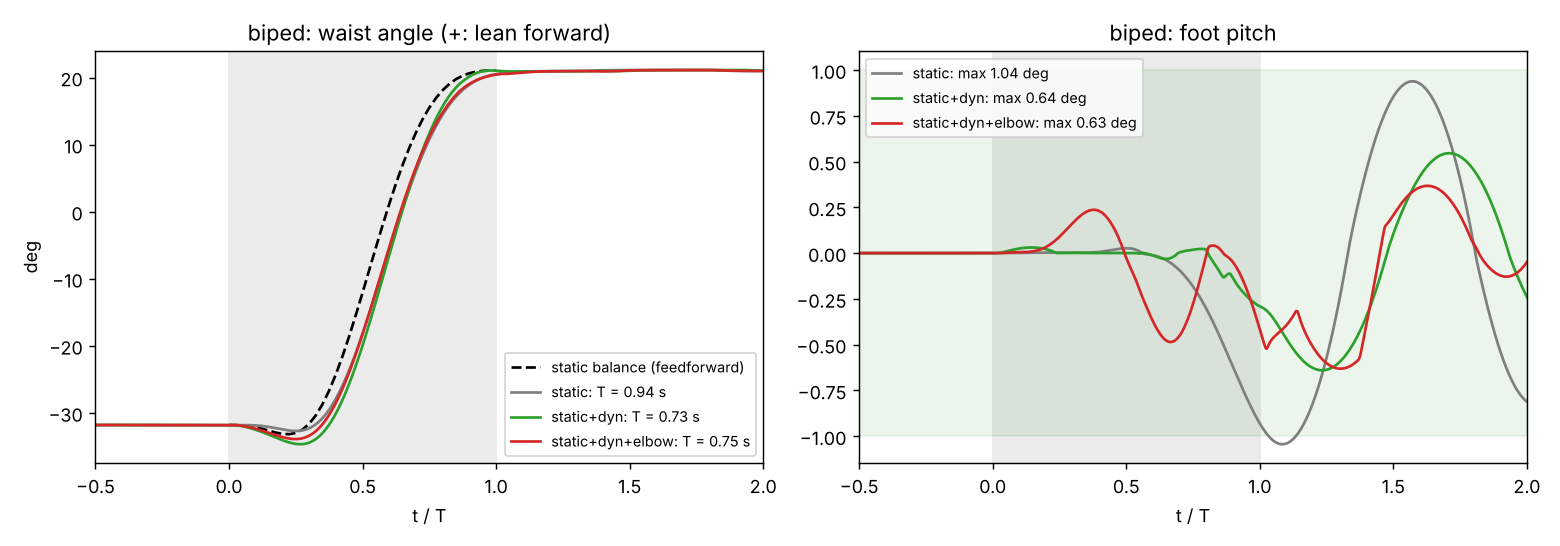
\includegraphics[width=0.86\textwidth]{field/field09_biped.png}
\caption{二本脚と戦車型の荷物運び（段階 9）。腰を使わない二本脚は、荷物を頭上から後ろへ回す途中で重心が足裏の外に出て倒れる。腰を使えば運べるが、同じ腰を持つ戦車型の方が速い。}\label{fig:biped}
\end{figure*}

\textbf{分かったこと}：
二本脚は、腕だけでは荷物運びができない。最初と最後の姿勢では静止できるが（重心は足裏の端から約 2 cm 内側）、途中で重心が足裏の外に出る。
Sim09 の「静止しても転倒」は安全余裕 2 cm を差し引いた判定で、物理的には「ぎりぎり立てる」状態だった。\textbf{2 層目の照合で 1 層目の判定の意味が正確になった}例である。
腰で上体を動かせば運べ（静的なつり合いで 0.94 s、補正を加えて 0.74 s）、\textbf{二本脚が立っていられるのは、脚ではなく、動かせる重い上体のおかげ}である。
それでも同じ腰を持つ戦車型の方が約 3 割速い。二本脚は静止の姿勢をつくるだけで上体を大きく傾ける必要があり、腰の可動域（±45°）の多くを「立つこと」に使ってしまうためである。
Sim09（関節の速度の上限あり）では差は 8\% だったが、速度の上限のないこの試験では、支持範囲の広さがそのまま速さの差になった。

\textbf{足裏の摩擦と足首}（段階 19、図~\ref{fig:lower1}(b)）：段階 9 の二本脚の脚の固定を外し、足（足裏 0.25 × 0.30 m）と足首の関節（ピッチ・ロール）を入れて、荷物運びで足が滑る・倒れる境目を測った。
\textbf{滑りの境目は前後・左右の滑りではなく、足裏の鉛直軸まわりのねじれで決まる}：段階 9 の最短の動作（0.735 s）は摩擦係数 0.88 が必要で、前後・左右の力からの予測 0.16 の 5.5 倍だった（F28）。
腕が体の横にあるため、振ると鉛直軸まわりの反作用が出て足がねじれて滑る。動作を 1.25 倍ゆっくりにすると必要な摩擦は 0.12 に下がる。
必要な足裏の大きさは 0.23 × 0.29 m（余裕なし）、足首のトルクは逆動力学の山の 1/3〜2/3 で足りた（山は短く、ZMP が一瞬外に出ても戻る。F29）。
誤差は、時間刻み ±10\%、摩擦円錐の近似 +40\%、回転子の慣性で 3 倍と大きく、\textbf{足元の校正値は接触のモデルの細部に敏感}である（上半身の段階 14 の「足元の摩擦の境目」と同じ）。
軽い足と硬いサーボの組は数値的に硬く、回転子の慣性を入れないと結果が時間刻みで変わった（F25）。接触のある機体では RK4 が発散し、implicitfast を使う（F26）。

\section{段差：人間大では脚、大型では履帯}\label{sec:steps}

地上で脚が有利なのは段差だろう、という予想を確かめた（Sim10、表~\ref{tab:steps}）。
戦車型（接地長 0.8 m）の越えられる段差は、履帯の前端の高さ（形の限界、0.25 m）と、摩擦の範囲で這い上がれるか（力の限界）の小さい方で決まる。
腕を前に伸ばして重心を前に移すと、力の限界は 0.26 → 0.33 m に上がる（地上版の能動的な質量バランス）。
二本脚は、上体を立てたままだと膝だけで体を持ち上げることになり 0.18 m が限界だが、\textbf{上体を前に傾けて重心を膝の上に寄せると 0.60 m} まで上れる。人が段差で前かがみになるのと同じで、ここでも重い上体を動かすことが効く。

\begin{table}[t]\centering\small
\caption{越えられる段差と大きさ（Sim10、トルクは $s^3$ の相似則）}\label{tab:steps}
\setlength{\tabcolsep}{3pt}
\begin{tabular}{lccc}\toprule
全高（倍率 $s$） & 戦車型 & 二本脚 & 有利 \\\midrule
約 0.9 m（0.5） & 0.12 m & 0.32 m & 脚 \\
\textbf{約 1.8 m（1、人間大）} & 0.25 m & \textbf{0.60 m} & \textbf{脚} \\
約 3.6 m（2） & \textbf{0.50 m} & 0.37 m & 戦車 \\
約 9 m（5） & \textbf{1.25 m} & 0.12 m & 戦車 \\
\textbf{約 18 m（10）} & \textbf{2.50 m} & 0.05 m & \textbf{戦車} \\\bottomrule
\end{tabular}
\end{table}

\textbf{大きさで逆転する}：戦車型は大きさによらず機体の 1/4 の段差を越える（形と摩擦はスケール不変）。
二本脚は、体を持ち上げるのに必要なトルクが $s^4$ で増えるのに、使えるトルクは $s^3$ でしか増えないため（第~\ref{sec:ambac} 節の二乗三乗則）、人間の 2 倍の大きさで戦車型に逆転され、18 m 級では 5 cm しか越えられない。
\textbf{脚の利点は人間大で最も大きく}、宇宙では大きさによらず有用（ただし遅い）、地上の段差では大型化で失われる。

\textbf{MuJoCo での履帯の段差}（段階 8・10）：板をつないだ履帯で、坂は摩擦の限界（31°）どおりに登れ、段差は長い履帯（1.2 m）で 0.30 m と短い履帯（0.8 m）の 2 倍だった。
短い機体は段の角で「シーソー」になり、機首が 49° まで上がって後ろに転倒した。腕を能動的に前に伸ばすと越えられる。
ただし長い履帯は旋回に 1.6 倍の力が要る（段階 11）。\textbf{用途に応じて形を選ぶ（アセンブル）}ことの具体的な数値である。

\textbf{MuJoCo で二本脚が段を上る}（段階 20、表~\ref{tab:steps20}、図~\ref{fig:lower1}(c)）：膝のある二本脚（Sim10 と同じ寸法、97 kg、矢状面に拘束）で、足を踏み出して段に乗り、片脚で体を持ち上げる動作を逆運動学で計画し、MuJoCo で実行した。
\textbf{上体の前傾は効く}（0.125 → 0.325 m、2.6 倍）が、高さは Sim10 の式の 55〜70\% だった。式が見落としていたのは、持ち上げ始めの姿勢で後ろの足が床に届かないこと、重心をつま先まで出すと足が前に倒れること（F33）、振り出す足が段の前面を越える道筋（F31）である。
後ろの足で床を蹴れば 0.52 m まで上れる。後ろの足のつま先が段の前面に触れて体重の 42\% を支え、「片脚で上った」ように見えた失敗もあった（F32、煙突登りと同じ）。
\textbf{大型化の逆転は Sim10 より早い}：$s=2$ では段の高さ 0 でも、膝を曲げて片脚で立って踏み出すだけでトルクの上限を超える（F34）。二乗三乗則は段を上る瞬間だけでなく、1 歩ずつに効く。

\begin{table}[t]\centering\small
\caption{二本脚が越えられる段の高さ [m]（段階 20、MuJoCo、片脚で持ち上げる）}\label{tab:steps20}
\setlength{\tabcolsep}{3pt}
\begin{tabular}{llccc}\toprule
$s$ & 上体 & Sim10 の式 & 準静的 & \textbf{MuJoCo} \\\midrule
1 & 立てたまま & 0.18 & 0.131 & 0.125 \\
1 & 前傾 & 0.60 & 0.350 & \textbf{0.325} \\
0.5 & 前傾 & 0.32 & 0.259 & 0.216 \\
2 & 前傾 & 0.37 & 不可 & \textbf{不可} \\\bottomrule
\end{tabular}
\end{table}

誤差は、計算・サーボ・接触・摩擦で ±2\%（二分法の 1 目盛り）以内、部品表の質量で 4.1\% だった。段の上りはトルクのつり合いで決まり、接触の細部に鈍い（足裏の滑りと対照的）。
ただし準静的な計画は 1 相 2 s より速いと平らな床でも倒れ、\textbf{速く動くには ZMP を計画に入れる}必要がある（次節の歩行の前提）。

\begin{figure*}[t]\centering
(a)\\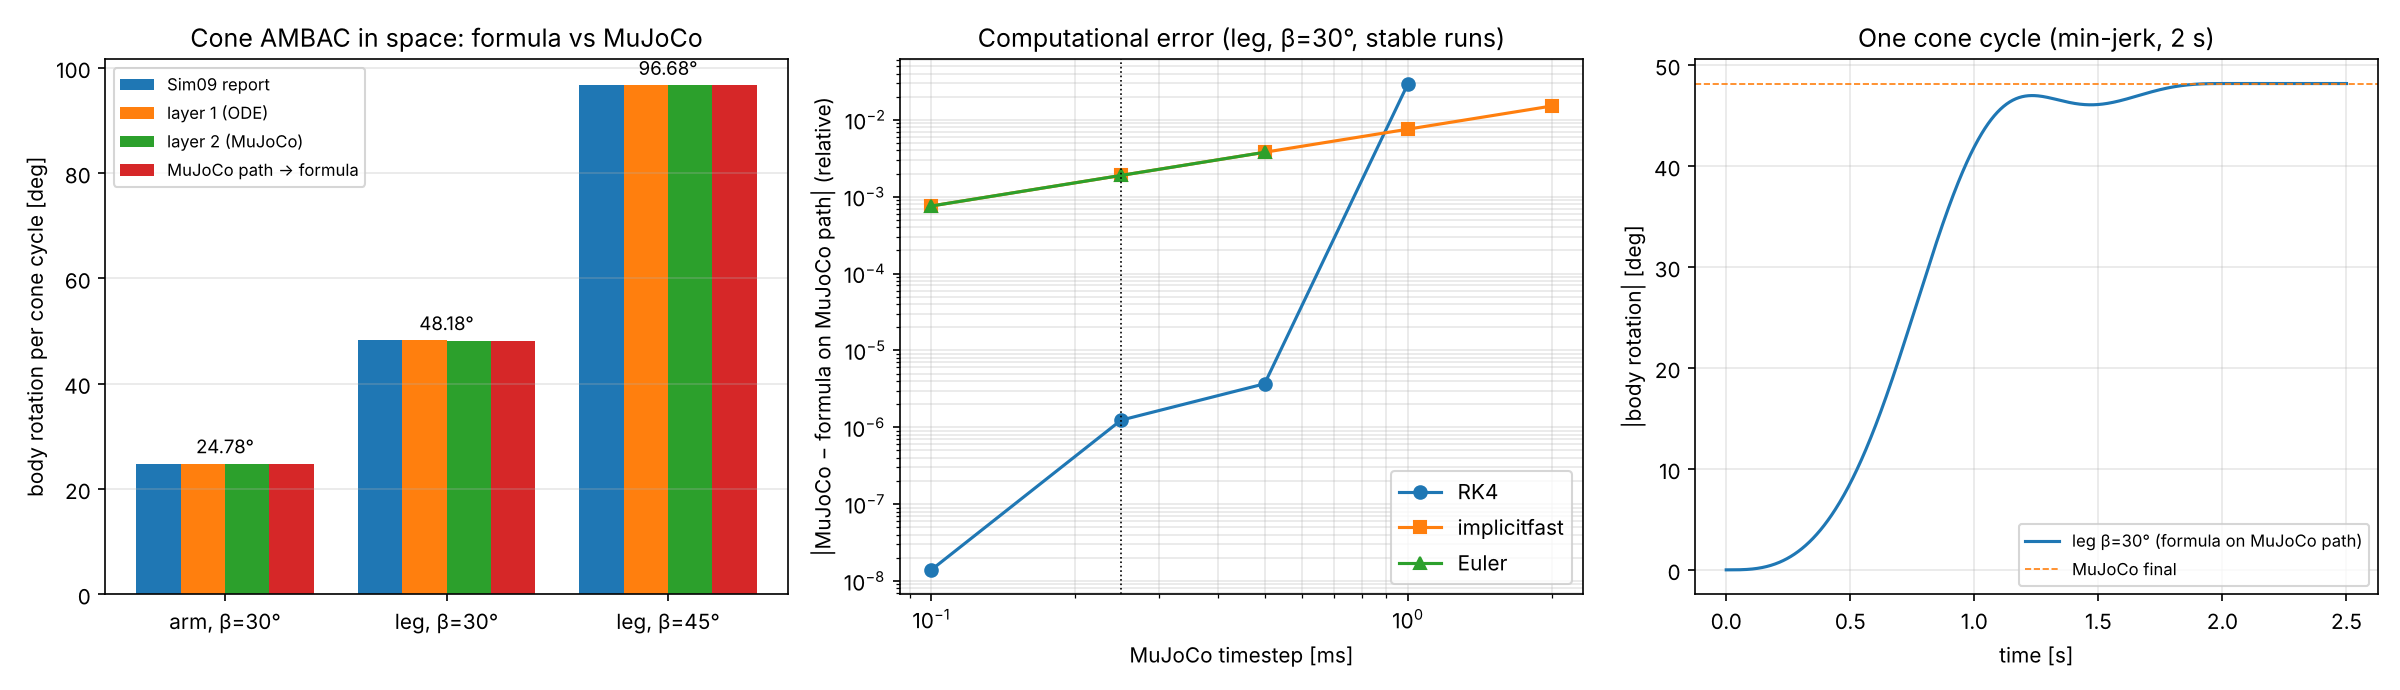
\includegraphics[width=0.9\textwidth]{field/field18_legcone.png}\\[0.4em]
\begin{minipage}[b]{0.37\textwidth}\centering(b)\\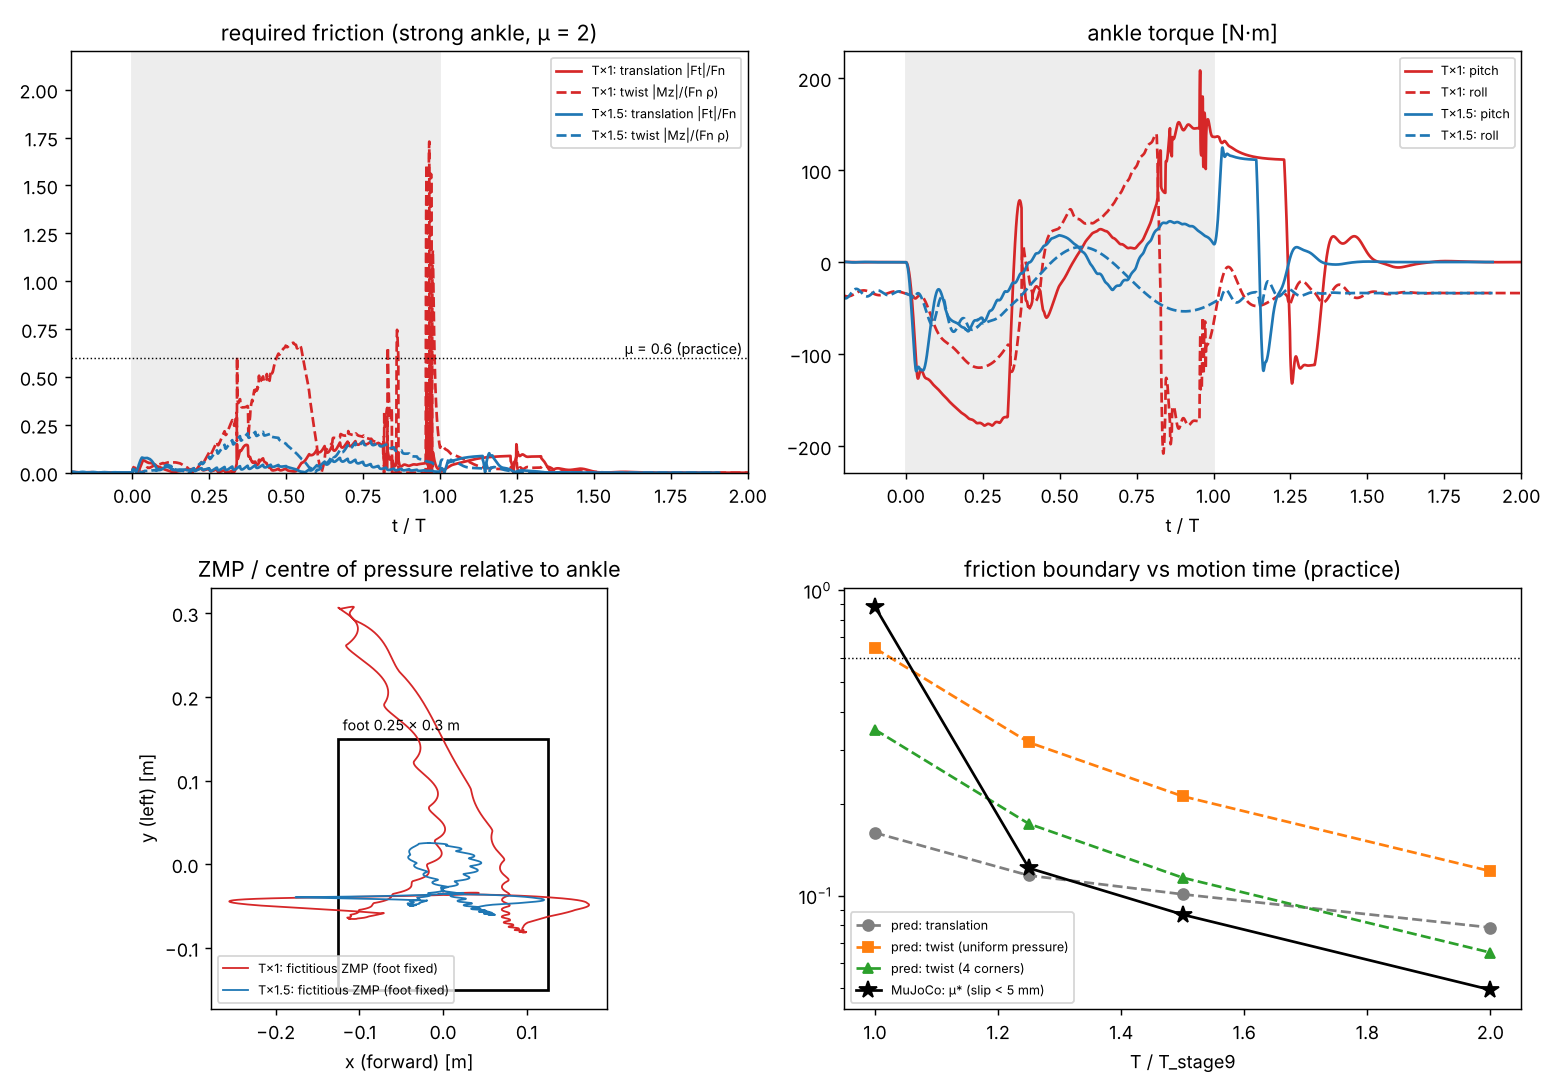
\includegraphics[width=\linewidth]{field/field19_ankle.png}\end{minipage}\hfill
\begin{minipage}[b]{0.61\textwidth}\centering(c)\\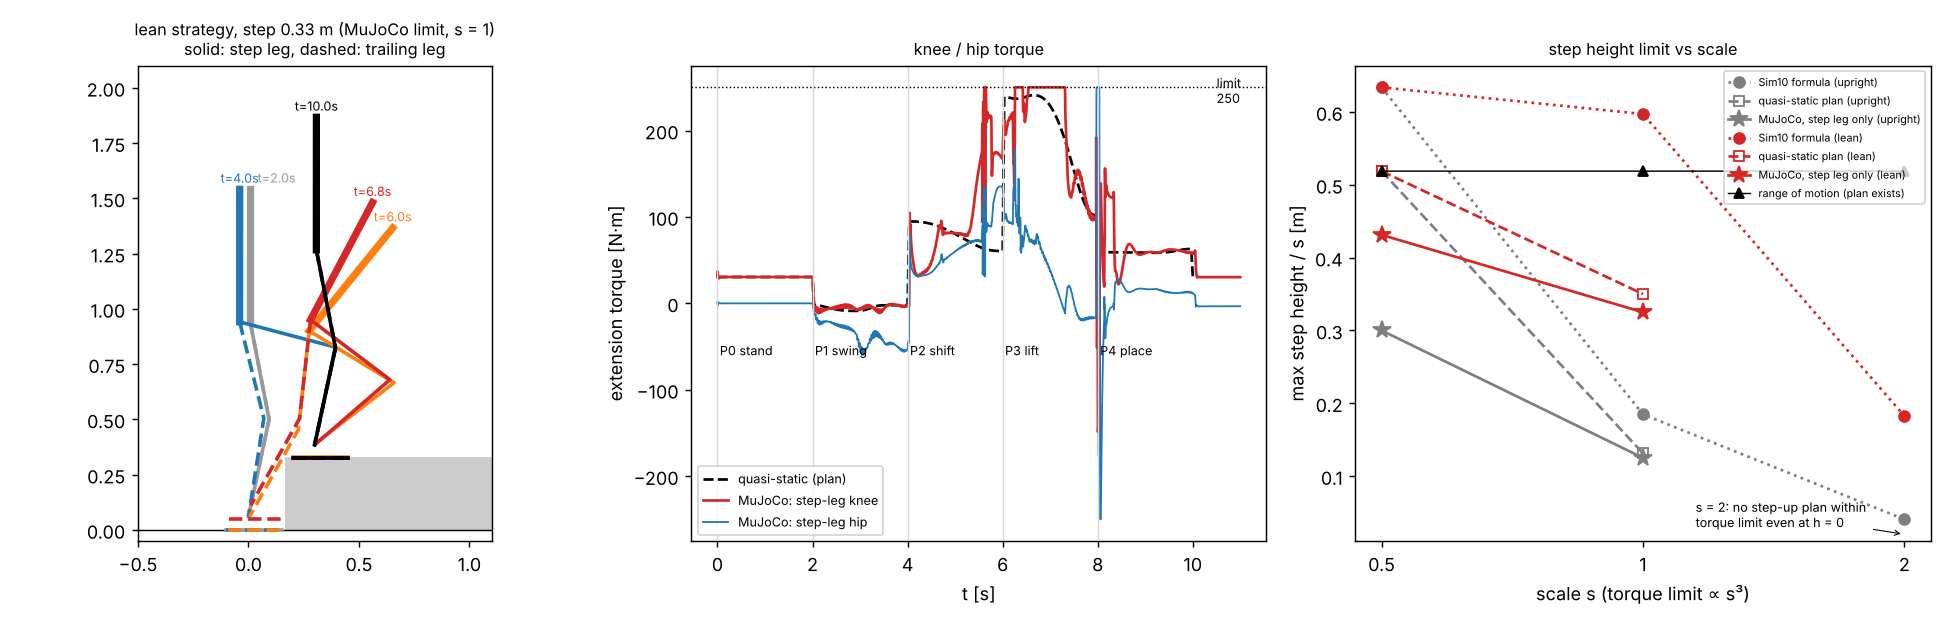
\includegraphics[width=\linewidth]{field/field20_biped_steps.png}\end{minipage}
\caption{下半身の MuJoCo での検証（1）。(a) 宇宙の脚の円錐（段階 18）：可動域と脚どうしの干渉を入れると 1 周 48.2° → 32.8°。(b) 足裏の摩擦と足首（段階 19）：滑りの境目は足のねじれで決まる。(c) 二本脚の段差（段階 20）：上体の前傾で 0.13 → 0.33 m。}\label{fig:lower1}
\end{figure*}

\section{歩行：開ループから、腕の振り・安定化・踏み出し・状態推定まで}\label{sec:walk}

第 3 版で「扱っていない」とした歩行を、段階 21〜26 で MuJoCo の 3 次元の二本脚（段階 20 と同じ寸法・質量、骨盤は自由関節で左右にも倒れる、片脚 5 自由度、足裏 0.25 × 0.10 m）で調べた（表~\ref{tab:walk}、図~\ref{fig:lower2}・\ref{fig:lower3}）。
計画は歩行の標準である線形倒立振子（LIPM）の ZMP プレビュー制御 \cite{kajita2003} で、関節角を位置サーボで追う。歩幅 0.25 m、8 歩を基準とした。

\begin{table}[t]\centering\small
\caption{歩行の段階（21〜26）の主な結果}\label{tab:walk}
\setlength{\tabcolsep}{2pt}
\begin{tabular}{@{}cp{0.27\linewidth}p{0.62\linewidth}@{}}\toprule
段階 & 仕組み & 主な結果 \\\midrule
21 & ZMP の計画（開ループ） & 歩ける。1 歩 0.64 s 以上は条件によらず成功。準静的の計画は 6 s/歩より速いと倒れる。0.48〜0.60 s/歩は足のねじれの滑りで失敗 \\
22 & 腕を脚と逆に振る & 成功の割合 0.62 → 1.00。必要な摩擦 1.11 → 0.38。逆向きに振ると悪化。最適な振り幅 25° \\
23 & DCM のずれ → 骨盤をずらす & 成功の割合 0.58 → 0.79。押されたときの前後の回復が capture point の $M\omega d$（39.5 N·s）に届く \\
24 & 押されたら踏み出す & 前後 40 → 50〜60 N·s（1 歩の理論値 73 の 7〜8 割）。横は単調でなく頼れない \\
25 & 重心の状態推定 & 差分の速度は全滅。LIPM＋足圧中心のカルマンフィルタとゲイン 0.3 で 0.71。足の場所を計画とみなすと 3 cm ずれる \\
26 & 脚のオドメトリ & 重心の位置の誤差 27 → 11 mm、成功の割合 0.83（真の値で動かす段階 23 は 0.79） \\\bottomrule
\end{tabular}
\end{table}

\textbf{準静的の計画では歩けない}（段階 21）：段階 20 と同じく「重心を支持する足の真上に置く」計画は、1 歩 1〜6 s のすべてで最初の体重移動で横に倒れた。
左右の足の間（0.2 m）を両脚支持の半分の時間で移る加速度で、ZMP が重心の真下から $z_c\ddot{y}/g$ ずれ、足の幅の半分（5 cm）を超えるためで、この見積もりが歩ける限界（5.91 s/歩）を MuJoCo（6.14 s）と 4\% で予測した（F36）。
ZMP の計画なら開ループでも 3 次元の二本脚が歩け、LIPM の ZMP と MuJoCo の足圧中心は 4.4 / 2.8 cm（RMS、前後 / 左右）で一致した。

\textbf{成功の地図は単調でない}（段階 21）：1 歩の時間を細かく変えると、0.40〜0.46 s は成功、\textbf{0.48〜0.60 s は失敗}、0.62 s 以上は成功だった。
失敗の中身は転倒ではなく、\textbf{支持する足が鉛直軸まわりに滑って向きが 20° ずれる}ことで、摩擦を 1.5 にするとほぼ消える。段階 19 の「滑りはねじれで決まる」が歩行でもそのまま現れた。
このため、限界を 1 つの数として求める二分法は、探す範囲によって 0.34 s にも 0.62 s にもなり（F37）、誤差の評価は時間の走査の「成功の並び」で行った。
速い側の成功は時間刻みや質量のわずかな違いで入れ替わり、Nelder--Mead 法で見つけた最速の 0.300 s にも再現性がない。
\textbf{第 III 部の課題「局所解・評価の平らさ」は、評価が平らになる形ではなく、成功の領域が島に分かれる形で現れた}。最適化の答えには、近くの条件での成功の割合を添える必要がある。

\textbf{歩くときの腕の振りは AMBAC である}（段階 22）：腕（片腕 4 kg、上体の質量の中から）を付け、計画の全身の鉛直軸まわりの角運動量から、足圧中心まわりのヨーのモーメントを最小にする振り幅を最小二乗で求めると、1 歩の時間によらず 23〜26° になった（人の腕の振りと同じ程度）。
この振り幅で脚と逆に振ると、\textbf{段階 21 の失敗の区間がすべて埋まり}（成功の割合 0.62 → 1.00）、1 歩 0.52 s で必要な摩擦は 1.11 → 0.38 に下がった。逆向きに振ると悪化し（0.46）、効いているのが角運動量を打ち消す向きであることを確かめた。
効果は時間刻み・腕の質量・サーボ・接触・摩擦・部品表の質量のどの条件でも正だった（質量 8 回で $+0.26\pm0.08$）。
宇宙で胴体の向きを変える AMBAC（第 I 部）と同じ仕組みが、地上の歩行では足裏のねじれを打ち消す役で現れる。\textbf{人が腕を振って歩くのは、上半身による AMBAC} という見方 \cite{collins2009} を、数値で裏づけた。

\textbf{閉ループの安定化と踏み出し}（段階 23・24）：DCM（capture point）$\xi = c + \dot c/\omega$ のずれに比例して骨盤を水平にずらす簡単な安定化 \cite{englsberger2015} で、歩ける範囲が広がり（成功の割合 0.58 → 0.79）、押されたときの前後の回復は capture point \cite{pratt2006} の理論値 $J_\mathrm{max}=M\omega d$（足首の戦略の限界、39.5 N·s）に届いた（開ループの 2〜4 倍）。
ゲインを上げすぎると 10 ms の制御周期で発振し（F41）、\textbf{重心の速度の測定に 5 cm/s の雑音を入れると全滅した}（F42）。実機に向けて最初に要るのは、制御の式よりも重心の状態推定である。
押されたら次の足を capture point の方へずらす踏み出しを加えると、前後は 50〜60 N·s に耐えた（1 歩で止まる理論値 73 N·s の 7〜8 割）が、横は単調でなく頼れなかった。
1 歩ずつ別々に直すと踏み出しすぎと逆向きの踏み出しが起こり（F43）、測った状態から計画し直すとかえって悪化した（F44）。\textbf{足の置き場所と重心の動きを同時に決めるモデル予測制御が要る}地点まで、簡単な仕組みで届く範囲を確かめたことになる。

\textbf{実機で測れる量からの重心の推定}（段階 25・26）：関節角（雑音 0.002 rad）、上体の IMU（傾き 0.002 rad、加速度 0.1 m/s$^2$）、足裏の力（足圧中心 1 cm）だけから重心の位置と速度を推定し、推定値で段階 23 の安定化を動かした（図~\ref{fig:lower3}）。
関節角から求めた重心の位置の 10 ms の差分を速度にすると、位置の誤差 2 mm でも速度の雑音が約 30 cm/s になり、24 通りの歩き方がすべて倒れた（F46、校正の F2 と同じ「雑音の入った測定値の微分」）。
LIPM の式 $\ddot c=\omega^2(c-p)$ を予測、測った足圧中心 $p$ を入力、運動学の位置を更新とするカルマンフィルタでは、真の値で最適だった $K=1$ では 0.25 にとどまり、$K=0.3$ に下げると 0.71 になった（F49：推定と制御は別々に最適化できない）。
上体の IMU の加速度を重心の加速度とみなすフィルタは、脚と腕が振れる分だけモデルの誤差になり、LIPM より悪かった（F48）。
残った誤差の主因は、\textbf{立っている足を計画どおりの場所とみなしたこと}で、雑音がなくても位置が約 3 cm ずれていた（F47）。
そこで段階 26 では、足裏の力で接地を判定し、着地した足の場所を「もう一方の足の推定の場所＋運動学で測った 2 つの足の差」で積み上げた（脚のオドメトリ）。
重心の位置の誤差は 27 → 11 mm、8 歩のあとの足の場所のずれは平均 21 mm で、成功の割合は 0.83 と、\textbf{真の値で動かした段階 23（0.79）以上}になった。
足の場所を正しく知るフィルタは 0.88 で、真の値の 0.79 を上回った。真の値で動かすことは上限ではなく、フィルタの遅れと平滑化が安定化の効き方を変えている（F52、見立て）。
最初の実装では計画の両脚支持の時刻に足の場所を更新したが、実際の両脚支持は 1〜2 ms しかなく、足の場所が 0.7 m ずれた（F50）。強いゲイン（$K=1$）では体が揺れて立っている足がねじれて滑り、オドメトリのずれが 93 mm まで積み上がった（F51）。
物理デバイスに要るのは、足裏の力センサ（接地の判定と足圧中心）、関節のエンコーダ、上体の IMU の 3 つで、関節角を微分しないこと、推定器とゲインを一緒に決めることが条件になる。

\textbf{大型化}：形が同じなら必要なトルク / 上限は $s$ に比例するはずで、$s=2$ では 1.9 倍とほぼその通りだった。$s=2$ で歩けたのは膝をほぼ伸ばした歩き方だけで、段階 20 の「大型では膝を伸ばした立ち方が必須」と合う。
ただし必要なトルクの最大値は着地の瞬間の短い山で、上限を 1.4 倍超えても歩ける場合があり、境目の予測には使えない（F38）。

\begin{figure*}[t]\centering
\begin{minipage}[c]{0.47\textwidth}\centering(a)\\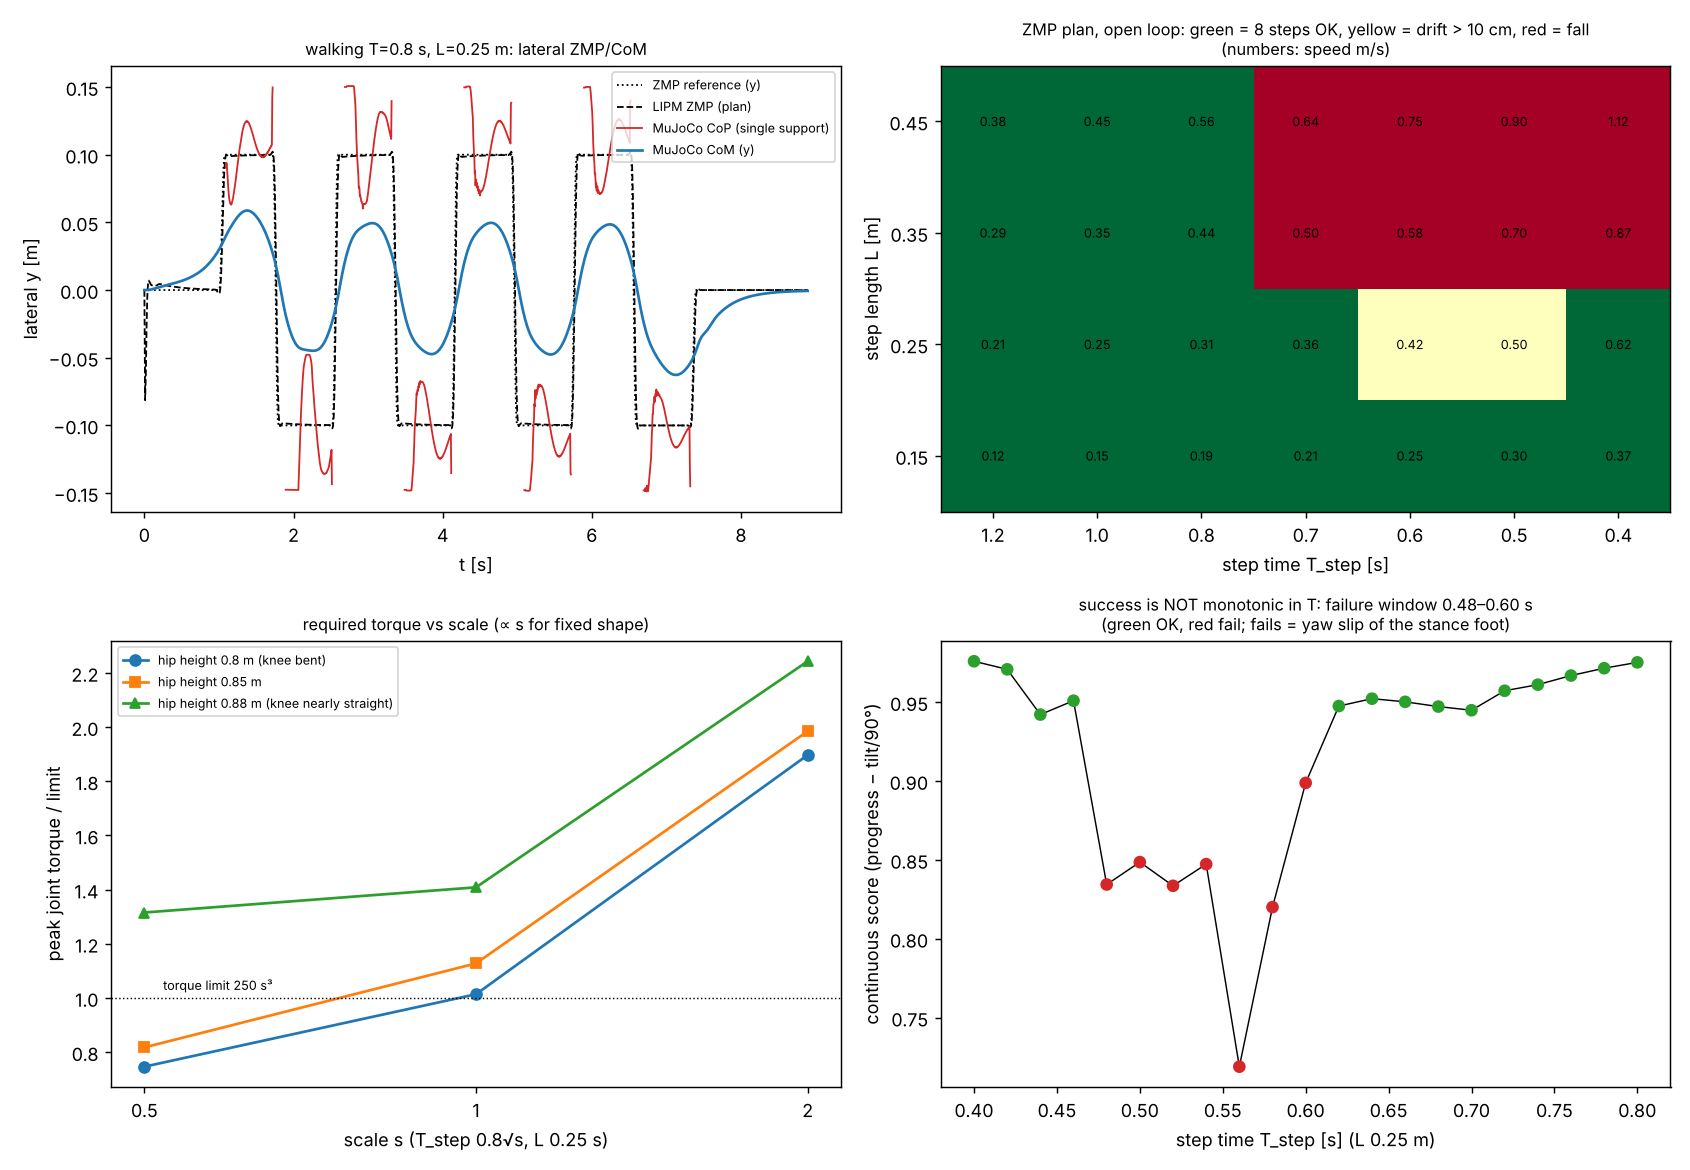
\includegraphics[width=\linewidth]{field/field21_walk.png}\end{minipage}\hfill
\begin{minipage}[c]{0.51\textwidth}\centering(b)\\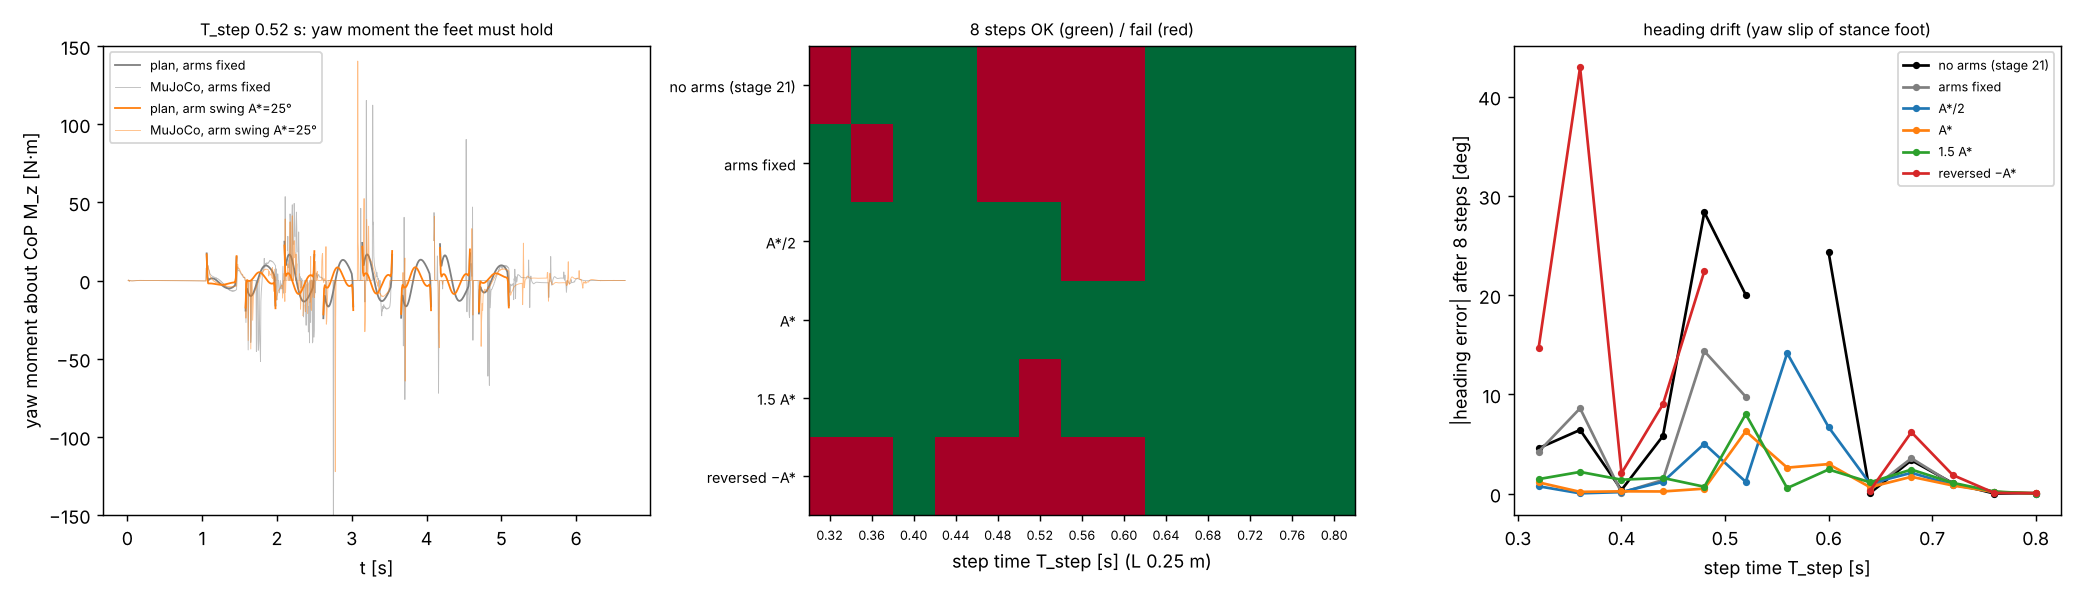
\includegraphics[width=\linewidth]{field/field22_armswing.png}\\[0.3em]
(c)\\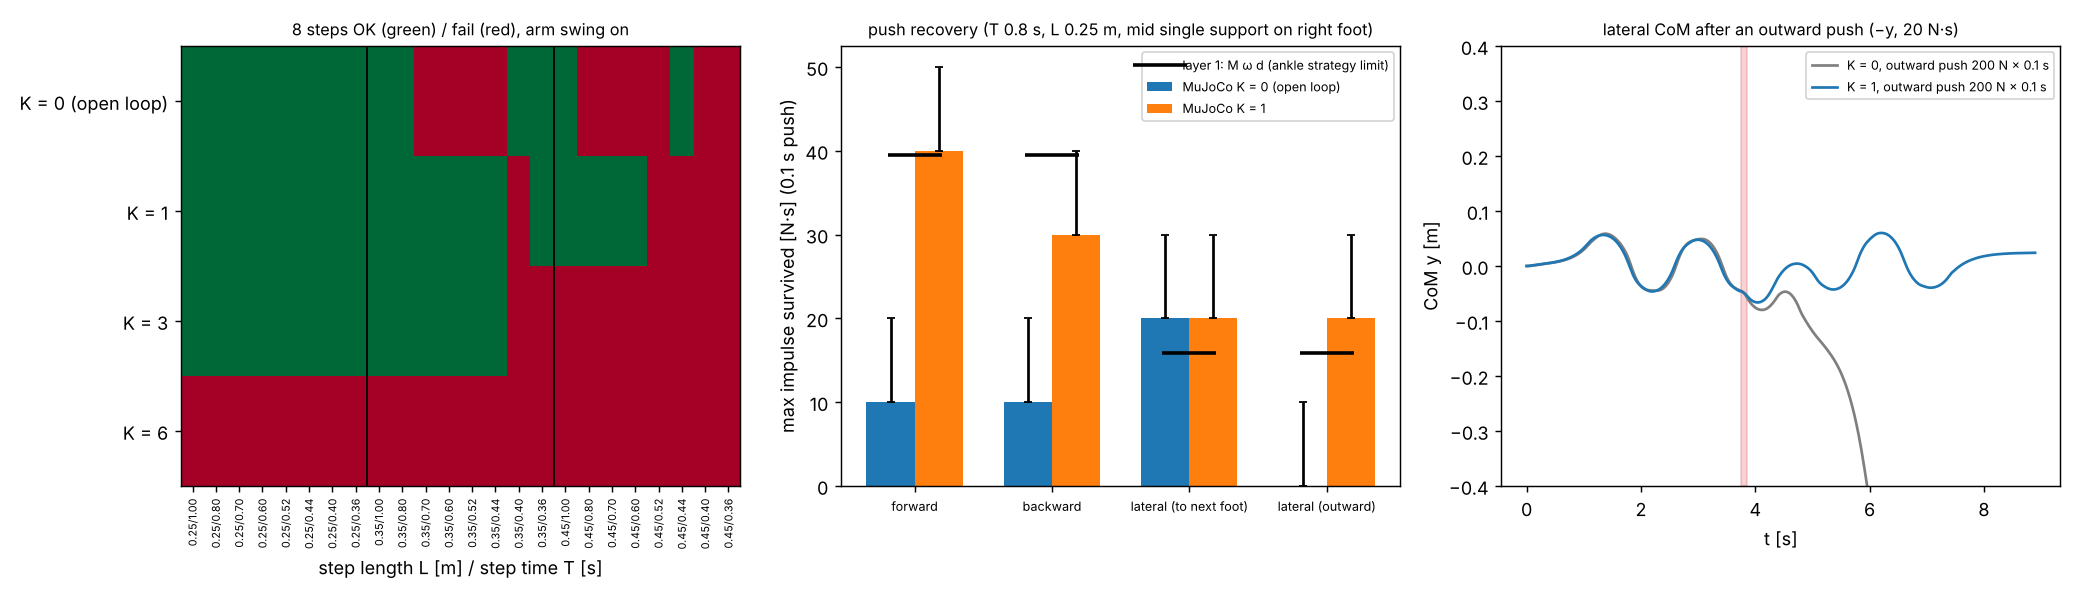
\includegraphics[width=\linewidth]{field/field23_stabilizer.png}\end{minipage}\\[0.4em]
(d)\\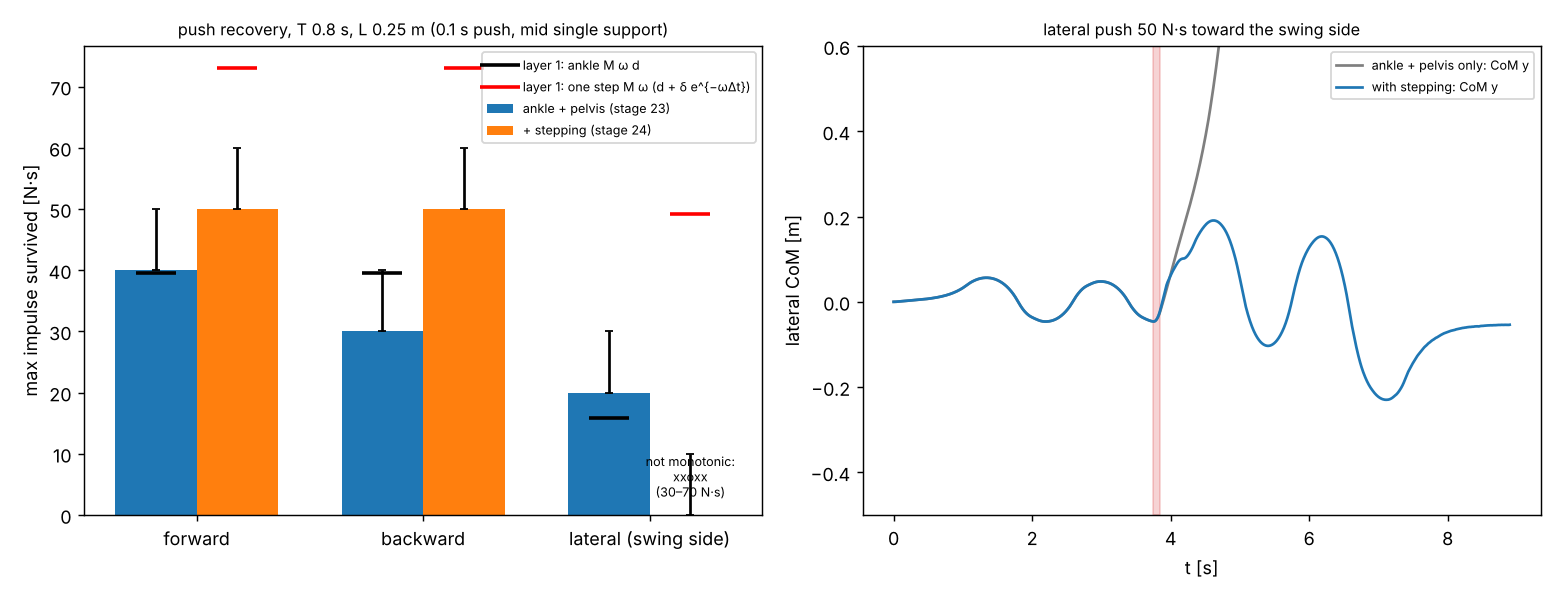
\includegraphics[width=0.62\textwidth]{field/field24_stepping.png}
\caption{下半身の MuJoCo での検証（2）：歩行。(a) ZMP の計画による開ループの歩行（段階 21）：成功の地図と、単調でない成功（0.48〜0.60 s/歩は足のねじれで失敗）。(b) 腕の振り（段階 22）：脚と逆に 25° 振ると失敗の区間が埋まり、逆向きは悪化。(c) 閉ループの安定化（段階 23）：押されたときの回復が capture point の予測に届く。(d) 踏み出し（段階 24）。}\label{fig:lower2}
\end{figure*}

\begin{figure*}[t]\centering
(a)\\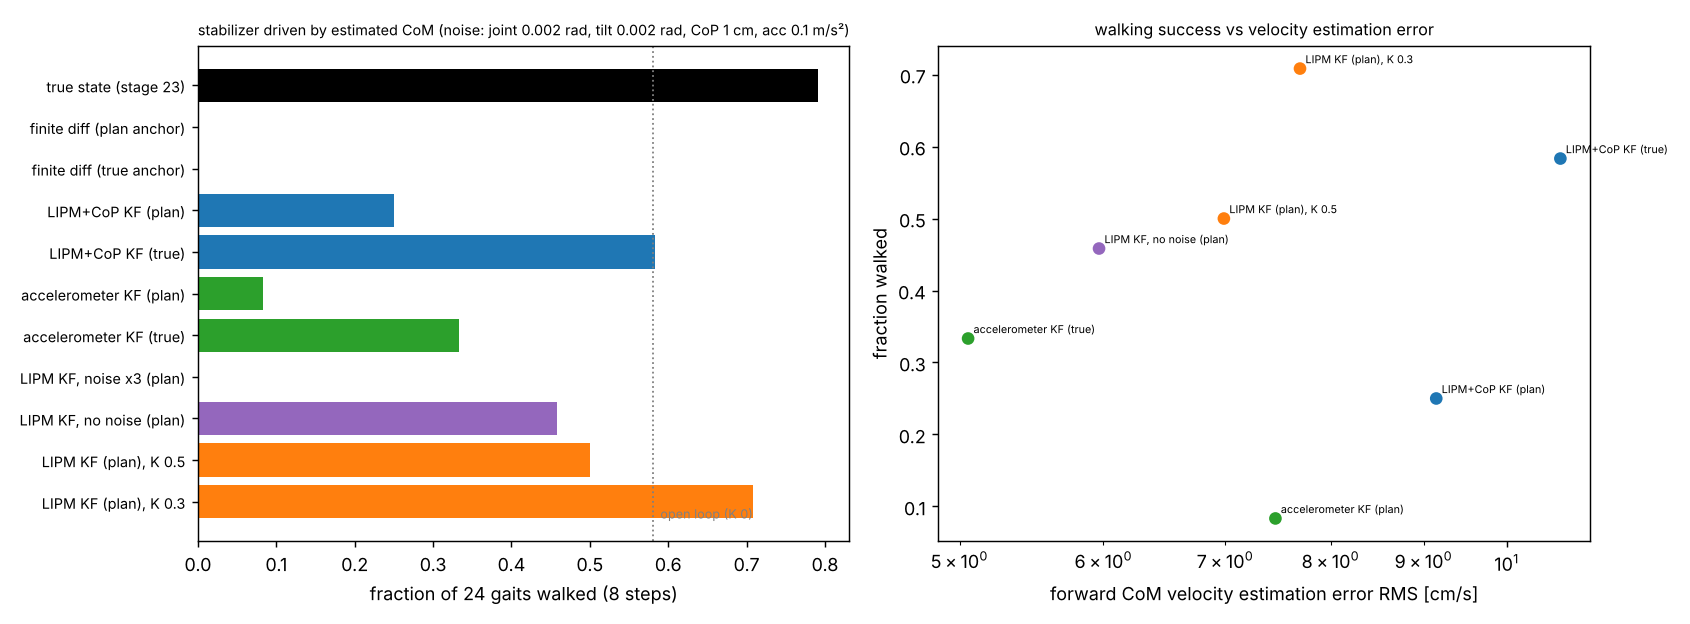
\includegraphics[width=0.78\textwidth]{field/field25_estimation.png}\\[0.4em]
(b)\\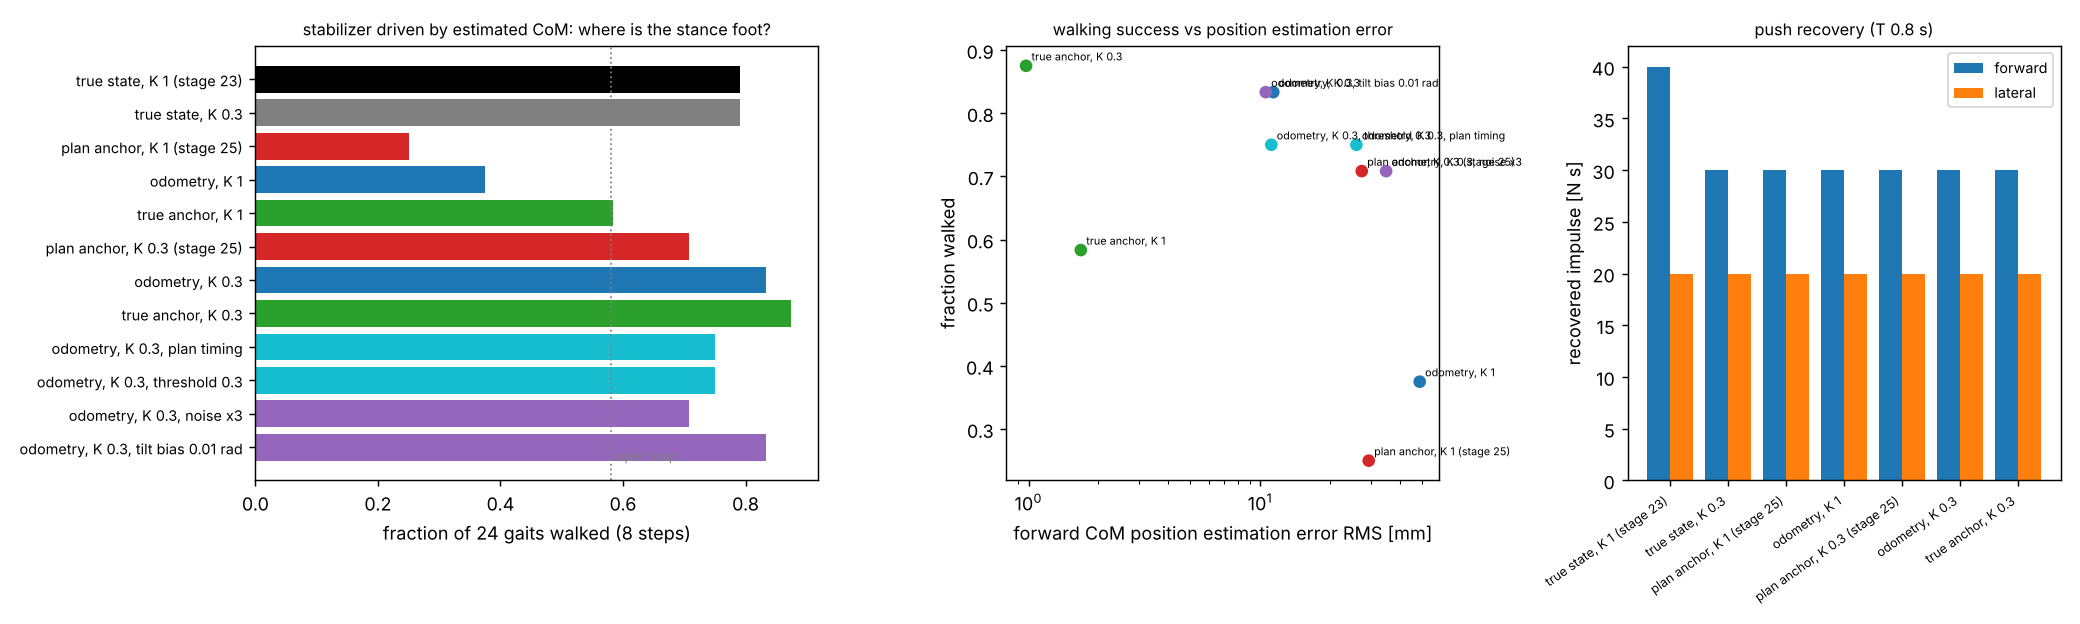
\includegraphics[width=0.98\textwidth]{field/field26_odometry.png}
\caption{下半身の MuJoCo での検証（3）：実機で測れる量からの重心の推定。(a) 段階 25：差分の速度は全滅し、LIPM＋足圧中心のカルマンフィルタはゲインを 0.3 に下げると 0.71。歩けるかどうかは速度の誤差の RMS だけでは決まらない。(b) 段階 26：脚のオドメトリで重心の位置の誤差が 27 → 11 mm になり、成功の割合は真の値で動かす場合（0.79）以上の 0.83。押されたときの回復は推定の方法によらずゲインで決まる。}\label{fig:lower3}
\end{figure*}

\section{下半身で残っている課題}\label{sec:lowerrem}

第 3 版で挙げた 5 つの課題のうち、歩行（第~\ref{sec:walk} 節）、宇宙の脚の 2 層目の照合（段階 18）、二本脚の段差（段階 20）、足元の校正値（段階 19）は MuJoCo で確かめた。
局所解の課題は、歩行で「成功の領域が島に分かれる」形で現れた（F37）。残っているのは次の点である。
\begin{enumerate}\setlength{\itemsep}{0pt}
\item \textbf{足の置き場所と重心の動きを同時に決める計画}（モデル予測制御）：横に押されたときの踏み出しと、複数歩で止まる動き（F43・F44）。
\item \textbf{立っている足の滑りの検出と、推定器・ゲインの同時の調整}：重心の推定と脚のオドメトリ（段階 25・26）で、実機で測れる量から歩けることは確かめた。残る誤差は立っている足のねじれの滑り（F51）で、上体の向き（ヨー）の推定と合わせて検出する必要がある。推定器・ゲイン・制御の周期を一緒に決める余地も残る（F49・F52）。
\item \textbf{3 次元の段差と、後ろの足で蹴る動き}：段階 20 は矢状面に拘束した。後ろの足で押す（0.52 m）動きを最初から計画に入れる。
\item \textbf{大型の歩き方}：$s=2$ で膝を伸ばした歩き方・歩幅を縮めた歩き方で、段差と歩行がどこまで戻るか。
\item \textbf{足元の接触のモデル}：足裏のねじれの滑りが、歩ける速さ（段階 21）と荷物運び（段階 19）の両方を決めた。MuJoCo の箱の接触は 4 隅でねじれを受け、一様な圧力の足裏より 1.85 倍強い（段階 19）。実物の足裏で測るべき最初の校正値である。
\end{enumerate}

\part{共通の土台：校正・誤差評価・実物との照合}

第 IV 部では、上半身・下半身に共通する土台として、校正値の推定とその誤差評価（第~\ref{sec:calib} 節）、うまくいかなかったことの記録（第~\ref{sec:fail} 節）、実物との照合を始める最小の実験（第~\ref{sec:bangai} 節）を扱う。

\section{課題 3：校正値を実機の前に設計する}\label{sec:calib}

\subsection{答えを隠した仮想の実機}
実機の代わりに、腕・脚の質量（$\pm15\%$）と胴体の慣性（$\pm10\%$）を乱数でずらした機体を作り、正解を推定する側に隠した（総質量 76 kg は既知とする）。
曲率マップの異なる場所に置いた 6 種類のループを 1 周ずつ回し、ジャイロ（雑音 0.2°/s、一定のバイアス最大 $\pm0.2$°/s）とエンコーダ（雑音 0.05°）を 100 Hz で模擬記録して、推定結果を正解と比べた。
推定法は、(a) 1 周ごとの正味の回転だけ、(b) 周回中の角速度の波形（関節角を微分して $\dot{\bm q}$ を求める）、
(b$'$) 式~(\ref{eq:ambac}) が時間を含まないことを利用し、0.1 s の区間ごとの回転量を $-\int\bm\Gamma\cdot d\bm q$ と比べる（微分なし）、
(c) (b) に関節トルクの情報を加える、の 4 つである。いずれもジャイロのバイアスを同時に推定する。

\begin{figure*}[t]\centering
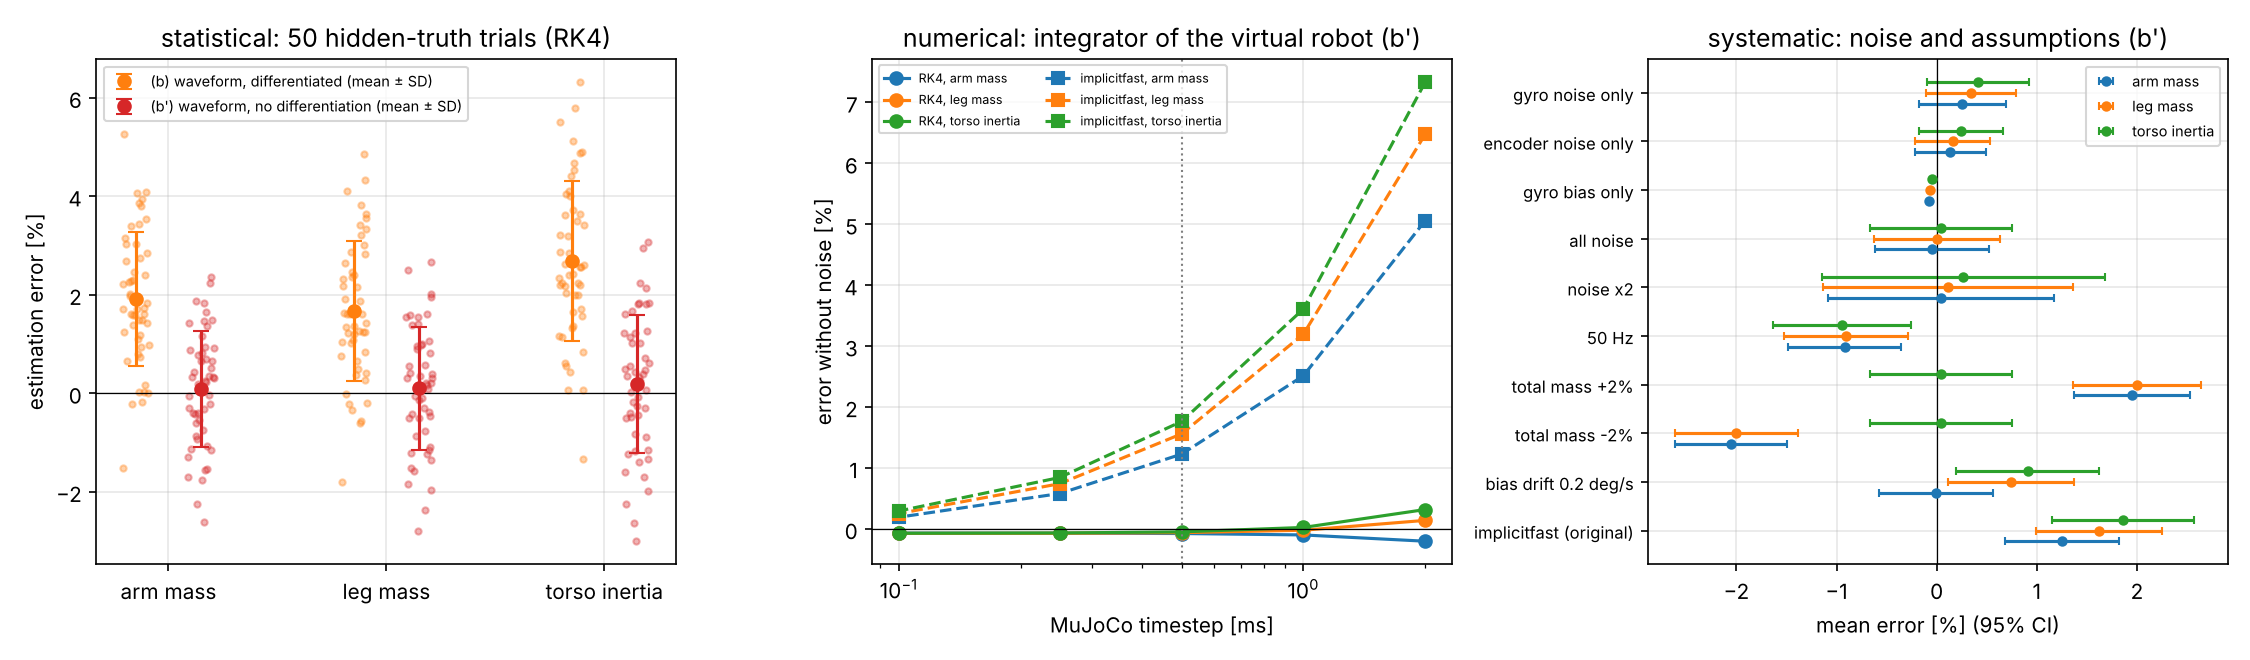
\includegraphics[width=0.84\textwidth]{figs/error_budget.png}
\caption{答えを隠した仮想の実機による校正の誤差評価。左：統計誤差（正解と雑音を変えた 50 回の試行、点は各試行、誤差棒は平均 $\pm$ 標準偏差）。
中：計算誤差（雑音なしの推定誤差と、仮想の実機の時間刻み・積分法。点線は既定の 0.5 ms）。
右：系統誤差（雑音の種類と推定側の仮定を 1 つずつ変えたときの平均の偏り、誤差棒は 20 通りの雑音による 95\% 信頼区間）。}\label{fig:calib}
\end{figure*}

\subsection{誤差の評価：統計・計算・系統}\label{sec:calib-err}

\begin{table}[t]\centering\small
\caption{推定誤差（平均 $\pm$ 標準偏差 [\%]、腕 / 脚 / 慣性）。(a)(b) は field04b の 50 回。(b$'$) は独立な 2 標本（field04b・04c）をまとめた 100 回で、平均の 95\% 信頼区間の半幅は 0.27〜0.32\%。}\label{tab:calib}
\footnotesize\setlength{\tabcolsep}{2pt}
\resizebox{\linewidth}{!}{\begin{tabular}{lccc}\toprule
推定の方法 & 腕 & 脚 & 慣性 \\\midrule
(a) 正味の回転 & $-7\pm28$ & $+103\pm145$ & $+16\pm42$ \\
(b) 微分 & $+1.9\pm1.4$ & $+1.7\pm1.4$ & $+2.7\pm1.6$ \\
(b$'$) 微分なし & $\bm{-0.01\pm1.37}$ & $\bm{+0.00\pm1.45}$ & $\bm{+0.07\pm1.63}$ \\
kinematic fit（第~\ref{sec:calib-kinfit} 節） & $\bm{-0.01\pm1.09}$ & $\bm{+0.04\pm1.14}$ & $\bm{+0.04\pm1.29}$ \\\bottomrule
\end{tabular}}
\end{table}

\begin{table}[t]\centering\small
\caption{(b$'$) の誤差の内訳 [\%]（腕 / 脚 / 慣性）}\label{tab:budget}
\setlength{\tabcolsep}{3pt}
\begin{tabular}{p{0.52\linewidth}c}\toprule
誤差の種類 & 大きさ \\\midrule
\multicolumn{2}{l}{\textbf{統計誤差}} \\
\quad 1 試行の標準偏差（100 回） & 1.37 / 1.45 / 1.63 \\
\quad \quad 標本 04b / 04c（各 50 回） & 1.2--1.4 / 1.5--1.8 \\
\quad 100 回の平均の 95\% 信頼区間 & $\pm$0.27 / 0.28 / 0.32 \\
\multicolumn{2}{l}{\textbf{計算誤差}（雑音なし）} \\
\quad 時間刻み 0.5→0.1 ms（RK4） & 0.02 以下 \\
\quad 最適化の収束条件 & 0.001 以下 \\
\quad 推定式の離散化・モデル差 & $-0.07$ \\
\quad 積分法 implicitfast（0.5 ms） & \textbf{+1.2 / +1.6 / +1.8} \\
\multicolumn{2}{l}{\textbf{系統誤差}（20 通りの雑音の平均）} \\
\quad 雑音による偏り（全雑音） & $-0.05$ / 0.00 / +0.05 \\
\quad 総質量の仮定 $\pm2\%$ & $\pm2.0$ / $\pm2.0$ / 0.0 \\
\quad バイアスのドリフト 0.2°/s & 0.0 / +0.7 / +0.9 \\
\quad サンプリング 50 Hz & $-0.9$ / $-0.9$ / $-0.9$ \\
\quad サンプリング 200 Hz & 0.0 \\\bottomrule
\end{tabular}
\end{table}

\textbf{統計誤差}（図~\ref{fig:calib} 左、表~\ref{tab:calib}）：ループ 1 周の正味の回転だけ (a) では、脚の質量を推定できなかった。
波形を使う (b) と (b$'$) の 1 試行のばらつきは主にジャイロの雑音による（ジャイロの雑音だけで 1.0\%）。
(b$'$) の平均は 0.1\% 以下で、95\% 信頼区間が 0 を含み、偏りは統計的に有意でない。

\textbf{本版での再評価：ばらつきの見積もりそのものの揺らぎ}：
レター \cite{letter2026} では (b$'$) の 1 試行のばらつきを、誤差評価のための 50 回（field04b）から 1.2〜1.4\% と報告した。
ところが、kinematic fit の評価（field04c）でも、同じ条件（RK4、0.5 ms、同じ雑音とバイアスの設定）で別の乱数の 50 回について (b$'$) を計算しており、そちらでは 1.5〜1.8\% だった。
2 つの標本の分散の比は 1.71〜1.74 で、ブートストラップの 95\% 区間は 1.01〜2.88、比が 1 を下回る割合は 2\% だった（約 2$\sigma$ の食い違い）。
外れ値によるものではなく（中央絶対偏差でも同じ傾向）、誤差の大きさとバイアスの大きさにも相関はなかった（相関係数 0.03〜0.06）。
条件の違いは見つからず、最も単純な解釈は、50 回の標本では 1 試行の標準偏差そのものが 10\% 程度揺らぎ、その揺らぎの端どうしを比べた、というものである。
そこで本稿では 2 標本をまとめた 100 回の値（1.37 / 1.45 / 1.63\%）を採用し、レターの「1.2〜1.4\%」は過小評価側だったと訂正する（\texttt{sims/field04d\_dispersion\_pool.py}）。
これは、後述の F4（5 回の試行での過小評価）と同じ種類の誤りが、50 回でも小さな形で残りうることを示す。

\textbf{系統誤差}（図~\ref{fig:calib} 右、表~\ref{tab:budget}）：(b) は +1.7〜2.7\% 偏り、信頼区間は 0 を含まない。偏りはエンコーダの雑音だけでも生じ、サンプリングを 200 Hz に上げると +3〜7\% に増え、雑音を 2 倍にしても増えた。
雑音の入った関節角を微分して推定式に入れると偏る errors-in-variables の典型であり、微分を避けた (b$'$) にはこの偏りがない。
推定側の仮定では、既知とした総質量の誤差が腕・脚の質量にそのまま 1:1 で移り、バイアスのドリフトとサンプリングの粗さが 1\% 弱の偏りを生んだ。

\subsection{計算誤差：シミュレータ自身が系統誤差の源になる}
当初、仮想の実機は部品表から組み立てた MuJoCo のモデルを既定の積分法 implicitfast（1 次）で計算しており、元の 5 回の試行では (b$'$) の誤差が 5 回ともプラス側にそろっていた（平均 +1.6〜2.3\%、ばらつき 0.5\%）。
「誤差約 2\%」の大部分は、偶然のばらつきではなく系統的な偏りだった。
雑音を除いても +1.2〜1.8\% の偏りが残り、偏りは時間刻みに比例した（2 ms で +5〜7\%、0.5 ms で +1.2〜1.8\%、0.1 ms で +0.2〜0.3\%）。
原因は、1 次の積分法で角運動量 $L=0$ がわずかに保たれないことにある。式~(\ref{eq:ambac}) からのずれは姿勢の角速度の 0.02\% 程度にすぎないが、
推定はこのずれを、次に述べる推定しにくい方向（全体の大きさ）に沿って吸収するため、パラメータでは 2 桁大きい偏りになる。
第 1 段階の手作りの機体は RK4 で計算していたため、段階 1 の照合ではこの問題は現れなかった。
積分法を RK4 にすると、0.5 ms でも雑音なしの誤差は 0.08\% 以下になった。
\textbf{答えを隠した仮想の実機で校正を設計するとき、仮想の実機自身の数値誤差が、推定しにくい方向で拡大されて系統誤差として現れる}。
これを見逃すと、推定法の限界や前処理の問題と取り違える（我々も当初は、偏りの原因を前処理だけに帰していた。第~\ref{sec:fail} 節 F5）。

\textbf{推定しにくい方向}：腕・脚の質量と胴体の慣性が\textbf{そろって同じ割合で増減する方向}が推定しにくい（特異値がほかの方向の約 1/60、推定の相関係数 0.99 以上）。
式~(\ref{eq:ambac}) は質量・慣性の「比」しか含まないため、姿勢の波形だけでは全体の大きさが決まらない。
これはマニピュレータの同定で知られる「推定可能なパラメータの組み合わせ」\cite{gautier1990} と同じ構造で、
総質量の誤差が質量の推定に 1:1 で移ることも、この構造の表れである。\textbf{絶対値を決めるには、総質量の正確な計量か、関節トルクなどの力の情報が要る}。
ただし力の情報を関節角の 2 回の微分と組み合わせると（推定法 (c)）、上と同じ理由で偏る（元の条件の 5 回の試行で、誤差は 4〜5\% に悪化した）ため、速度・加速度を直接測るセンサーとの組み合わせが必要になる。

\subsection{拘束条件つきの当てはめによる誤差の自己評価}\label{sec:calib-kinfit}
実機では正解が分からないため、校正値そのものに加えて「その値をどこまで信じてよいか」を、1 回の校正から示せる必要がある。
そこで、素粒子実験の kinematic fit \cite{avery1998} の考え方を校正に持ち込んだ。
関節角も誤差のある測定値として、その誤差の範囲で動かし、角運動量 $L=0$ を拘束条件として厳密に満たすように、真の関節角の列 $\bm Q$・パラメータ $\bm p$・ジャイロのバイアス $b$ をまとめて当てはめる。
{\small\begin{equation}
\chi^2=\sum_i\frac{\|\bm Q_i-\bm q_{m,i}\|^2}{\sigma_q^2}+\sum_i\frac{\bigl(\omega_{m,i}-b+\bm\Gamma(\bm Q_i;\bm p)\cdot\dot{\bm Q}_i\bigr)^2}{\sigma_\omega^2}
\label{eq:kinfit}
\end{equation}}
$\dot{\bm Q}_i$ は当てはめた $\bm Q$ の中心差分で、雑音の入った測定値を微分しないため、(b) のような偏りは生じない。
未知数は約 5200 個だが、ヤコビアンが疎なので、CPU で 1 回 50 s 程度で解ける。
得られた共分散から、推定ごとの誤差 $\sigma$ と、当てはまりの良さ $\chi^2$ が得られる。

\begin{figure*}[t]\centering
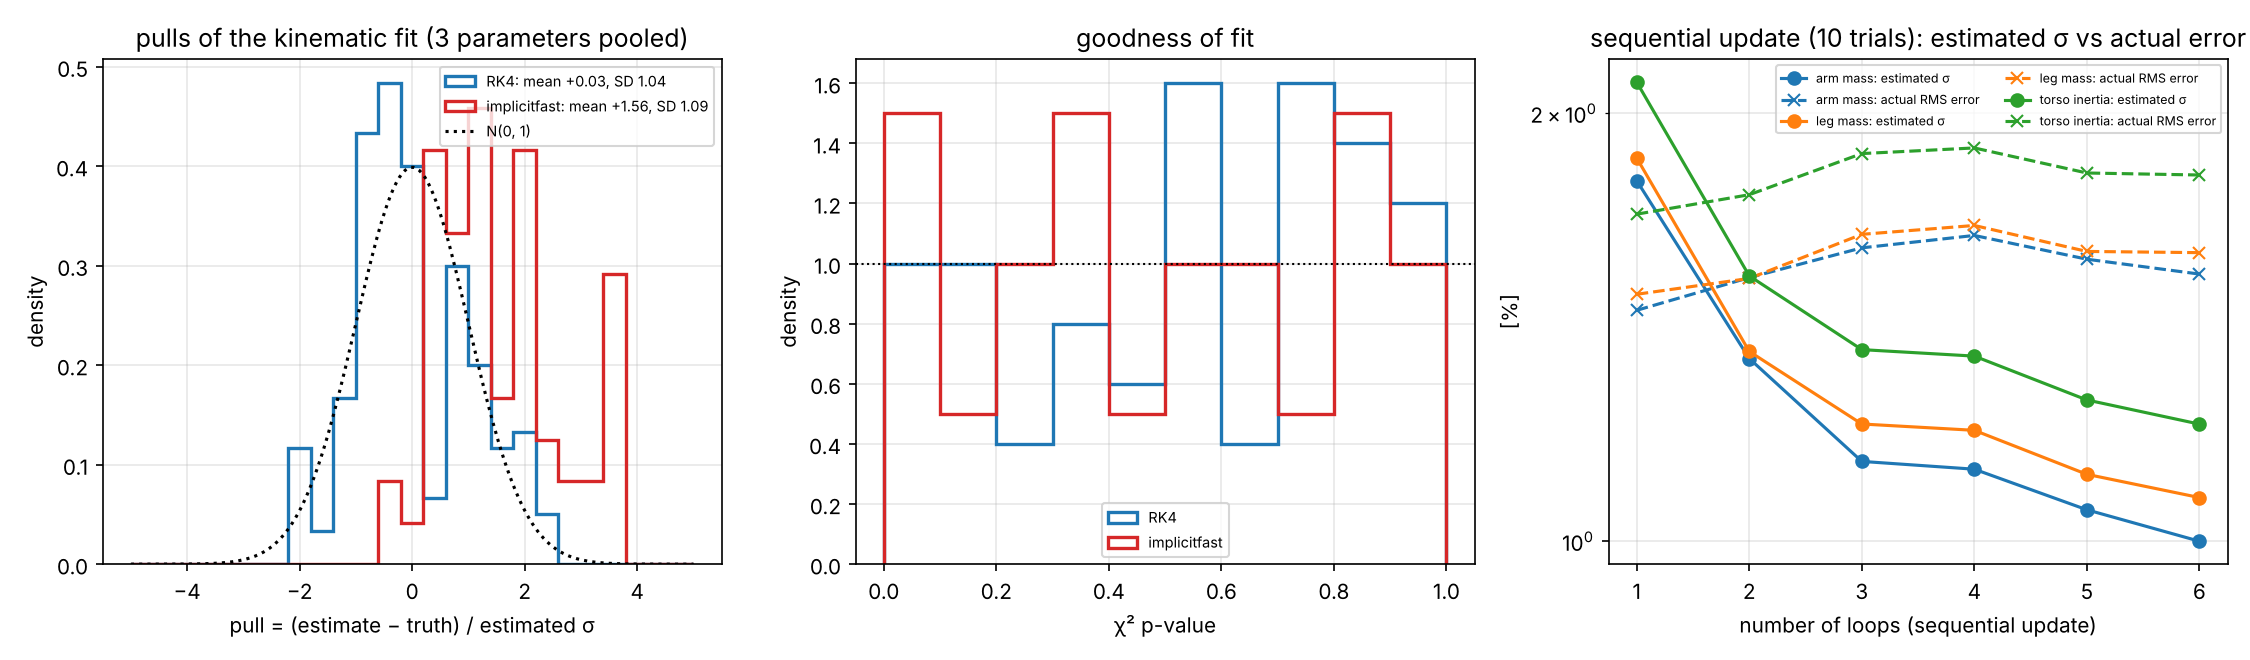
\includegraphics[width=0.84\textwidth]{figs/kinfit.png}
\caption{拘束条件つきの当てはめ（式~(\ref{eq:kinfit})）の自己評価。左：pull $=(\text{推定}-\text{正解})/\sigma$ の分布（3 つのパラメータをまとめた）。RK4 の仮想の実機（50 回）では $N(0,1)$ に一致し、積分法の系統誤差を含む implicitfast（20 回）では $+1.6\sigma$ ずれる。
中：$\chi^2$ の p 値。どちらも一様で、系統誤差は $\chi^2$ に現れない。右：ループを 1 本ずつ加える逐次更新での、推定した $\sigma$（実線）と実際の誤差の二乗平均（破線、10 回）。}\label{fig:kinfit}
\end{figure*}

\begin{table}[t]\centering\small
\caption{kinematic fit の自己評価（腕 / 脚 / 慣性）}\label{tab:kinfit}
\footnotesize\setlength{\tabcolsep}{2pt}
\resizebox{\linewidth}{!}{\begin{tabular}{lcc}\toprule
 & RK4（50 回） & implicitfast（20 回） \\\midrule
誤差の平均 [\%] & $-0.01$ / $+0.04$ / $+0.04$ & $+1.5$ / $+1.8$ / $+2.1$ \\
誤差の標準偏差 [\%] & 1.09 / 1.14 / 1.29 & 1.09 / 1.18 / 1.34 \\
推定した $\sigma$ の平均 [\%] & 1.04 / 1.11 / 1.25 & 1.07 / 1.15 / 1.29 \\
pull の平均 & $+0.01$〜$0.05$ & $+1.4$〜$1.6$ \\
pull の標準偏差 & 1.04〜1.05 & 1.10〜1.11 \\
$|\text{pull}|<1$ の割合 & 66〜68\% & 30〜40\% \\
$\chi^2/\text{ndf}$ & $0.997\pm0.032$ & $1.003\pm0.034$ \\
相関係数 & 0.989〜0.999 & 0.989〜0.999 \\\bottomrule
\end{tabular}}
\end{table}

結果を図~\ref{fig:kinfit} と表~\ref{tab:kinfit} に示す。RK4 の仮想の実機での 50 回の試行で、推定は偏らず（平均 0.04\% 以下）、ばらつきは 1.1〜1.3\% だった。
同じ 50 回の試行で計算した (b$'$) と比べると、標準偏差の比は 0.70（ブートストラップの 95\% 区間 0.57〜0.87）で、\textbf{ばらつきは約 3 割小さい}。
この比較は同じデータに対する対応のある比較なので、前節で見た標本間の揺らぎの影響を受けない（別の標本の (b$'$) と比べると、減り方は 2 割程度に見える）。
\textbf{推定ごとの誤差 $\sigma$ は正しく見積もられ}、pull の平均は 0.01〜0.05、標準偏差は 1.04〜1.05、$|\text{pull}|<1$ の割合は 66〜68\% で、$\chi^2/\text{ndf}=0.997\pm0.032$ だった。

ループを 1 本ずつ加え、前の推定値と共分散を事前情報として当てはめ直す逐次更新（カルマンフィルタと同じ形で、素粒子実験の飛跡の当てはめ \cite{fruhwirth1987} でも用いられる）では、
$\sigma$ はループを加えるごとに 1.8\% から 1.0\% へ縮み、最終値は一括の当てはめと 0.23\% 以内で一致した。
なお、逐次更新を試した 10 回では実際の誤差の二乗平均（1.5\%）が $\sigma$（1.0\%）より大きく見えたが、同じ 10 回の一括の当てはめも 1.55\% で、この 10 回がたまたま誤差の大きい試行だった（F10）。結論は 50 回の pull で出す。

一方、積分法の系統誤差を含む仮想の実機では、pull は $+1.4$〜$1.6\sigma$ ずれたが、\textbf{$\chi^2$ の p 値は一様のままで、当てはまりの良さからは検出できなかった}。
3 つのパラメータの推定の相関係数が 0.99 以上あり、ずれが推定しにくい方向に吸収されるためである。
拘束条件つきの当てはめは誤差の自己評価を与えるが、推定しにくい方向の系統誤差は、正解の分かっている照合など独立な検証と組み合わせて評価し続ける必要がある。

\subsection{誤差評価から学んだこと}
\begin{enumerate}\setlength{\itemsep}{0pt}
\item \textbf{仮想の実機（シミュレータ）自身が系統誤差の源になる。} 保存則など答えの分かっている量で、仮想の実機の数値設定を先に検証する。
\item \textbf{推定しにくい方向は、小さな誤差を大きく拡大し、しかも $\chi^2$ に現れない。} 相関行列と pull を見る。
\item \textbf{誤差の原因を一度決めつけると、取り違える。} 原因は 1 つずつ切り分けて確かめる。
\item \textbf{誤差の見積もりにも誤差がある。} 少数試行のばらつきは過小にも過大にも出るので、独立な標本どうしを比べ、まとめた値と区間で報告する。
\item \textbf{拘束条件つきの当てはめは、推定値とその誤差を同時に与え、逐次更新できる}。フィジカル AI の校正の枠組みとして有望である。
\end{enumerate}


\section{うまくいかなかったこと}\label{sec:fail}

本節では、成功した結果だけでなく、うまくいかなかった試みとその理由を、先行研究や既知の事柄と対応づけて記録する（表~\ref{tab:fail}・\ref{tab:fail2}・\ref{tab:fail3}・\ref{tab:failidx}）。
表~\ref{tab:fail3} の F21〜F52 は、第 4・5 版で加えた下半身の MuJoCo での検証（段階 18〜26）のものである。
表~\ref{tab:fail2} の F14〜F19 は第~\ref{sec:bangai} 節の解析を合成データで確かめたとき、F20 は本版の作成時に見つけたものである。
先行研究と同じ形で失敗していれば、それは我々の仮説と論理が同じ道筋をたどっている証拠になる。

\begin{table*}[t]\centering\footnotesize
\caption{校正の誤差評価と論文化（2026 年 11 月 22〜26 日）でうまくいかなかったこと}\label{tab:fail}
\setlength{\tabcolsep}{3pt}
\begin{tabular}{cp{0.17\textwidth}p{0.19\textwidth}p{0.27\textwidth}p{0.27\textwidth}}\toprule
\# & 試みたこと & うまくいかなかったこと & 原因 & 先行研究・既知の事柄との対応 \\\midrule
F1 & 正味の回転だけで推定 (a) & 脚の質量が決まらない（$+103\pm145\%$） & 正味の回転は 6 個の数しか与えず、3 つのパラメータとバイアスを分けるには情報が足りない & 同定には十分に励起する入力と観測が要る（persistent excitation）。マニピュレータの励起軌道の設計と同じ \\
F2 & 関節角を微分して推定 (b) & +1.7〜2.7\% の有意な偏り。サンプリングを上げると +3〜7\% & 雑音の入った説明変数の微分を回帰に入れると偏る。微分で雑音が増幅される & errors-in-variables の偏り。総最小二乗法や、測定値自体を当てはめる方法（kinematic fit）が対策 \\
F3 & (b) に関節トルクを加える (c) & かえって悪化（4〜5\%） & 加速度を関節角の 2 回の微分で求めるため、F2 がさらに強く出る & 慣性パラメータ同定で加速度の推定が誤差の主因になること \cite{atkeson1986} \\
F4 & 5 回の試行でばらつきを見積もる & 0.5\% と過小評価（50 回では 1.2〜1.8\%） & 試行回数が少なく、偏りが支配的で、ばらつきが偏りに隠れていた & 少数試行での誤差の過小評価。素粒子実験で toy MC を多数回まわして pull を確かめる理由 \\
F5 & 「(b$'$) の偏りの原因は前処理」と結論 & \textbf{誤り}。主因は仮想の実機の積分法 & 雑音・積分法・時間刻みを 1 つずつ変える切り分けをせず、もっともらしい説明で止めた & 系統誤差は原因を 1 つずつ変えて確かめる（素粒子実験の系統誤差の評価の手順） \\
F6 & 組み立てた機体（implicitfast、0.5 ms）を仮想の実機にする & 雑音がなくても +1.2〜1.8\% 偏る（時間刻みに比例） & 1 次の積分法で $L=0$ がわずかに保たれず、そのずれが推定しにくい方向で 2 桁拡大される & 保存則を守らない積分法のドリフト（シンプレクティック積分法の動機）。ゲーム用物理エンジンの角運動量の扱いと同じ問題 \\
F7 & kinematic fit の $\chi^2$ で系統誤差を検出 & pull +1.5$\sigma$ の偏りが $\chi^2$ に現れない & 相関 0.99 以上で、ずれが推定しにくい方向に吸収される & 推定できないパラメータの組み合わせ（base parameters \cite{gautier1990}）。$\chi^2$ の良さは系統誤差がないことを保証しない \\
F8 & 絶対値を姿勢の波形だけで決める & 総質量の仮定の誤差が 1:1 で移る & 式~(\ref{eq:ambac}) が質量・慣性の比しか含まない & F7 と同じ構造。外部の計量か力の情報が必要 \\
F9 & kinematic fit を関数評価 200 回で解く & 上限で打ち切り（収束の保証なし） & 約 5200 個の未知数の収束が遅い & 大規模な当てはめでは収束の判定と反復の上限を確かめる。2000 回で収束を確認 \\
F10 & 逐次更新の 10 回で $\sigma$ と実際の誤差を比べる & 実際の誤差 1.5\% が $\sigma$ 1.0\% より大きく見えた & この 10 回がたまたま誤差の大きい試行（一括の当てはめも 1.55\%） & 少数試行の比較は誤解を生む（F4 と同じ）。結論は 50 回の pull で出す \\
F11 & レター論文に SF 考証を混ぜる & 「技術的な主張のノイズ」と指摘された & 読者と論証の種類が違う内容を 1 本にした & 学術論文と解説・考証の役割分担。2 本に分けて解決 \\
F12 & 画面のないクラウドで MuJoCo を描画付きで動かす & 描画ライブラリがなく起動しない & 環境に osmesa・egl がない & 計算だけなら描画を切って動く \\
F13 & 50 回の試行で (b$'$) のばらつきを 1.2〜1.4\% と報告（レター） & 同じ条件の別の 50 回では 1.5〜1.8\%（分散の比 1.7、約 2$\sigma$） & 50 回でも標準偏差の推定は 10\% 程度揺らぐ。1 つの標本だけで報告した & 誤差の誤差。独立な標本を比べ、まとめた値と区間で報告する（本版で訂正、第~\ref{sec:calib-err} 節） \\\bottomrule
\end{tabular}
\end{table*}

\begin{table*}[t]\centering\footnotesize
\caption{3 層目の照合の解析を合成データで確かめたとき、および本版の作成時にうまくいかなかったこと（2026 年 11 月 26 日）}\label{tab:fail2}
\setlength{\tabcolsep}{3pt}
\begin{tabular}{cp{0.17\textwidth}p{0.19\textwidth}p{0.27\textwidth}p{0.27\textwidth}}\toprule
\# & 試みたこと & うまくいかなかったこと & 原因 & 先行研究・既知の事柄との対応 \\\midrule
F14 & 2 台の時計のずれ $\tau$ をジャイロの相互相関のピークで決める & 回転の合成データで 21 ms ずれた（振り子では 0.5 ms） & 一方向に回る信号は平均が 0 でなく、記録の長さも違うので、ピークが重なりの量に引きずられる & 相関のピークは形の類似しか見ない。2 台目 $= a\cdot$（1 台目）$+c$ の残差を $\tau$ について最小にする仕上げで 0.1〜0.4 ms に \\
F15 & 実験 B を、各時刻の $\omega$ を未知数にして当てはめる（バイアスは自由） & $r$ が +1.7 mm（6σ）、+4.9 mm（15σ）偏った & $\omega$ 全体のずれとジャイロのバイアスの組は、加速度の $\omega^2$ の項でしか区別されず、ほぼ縮退する & F7・F8 と同じ推定しにくい方向。静止区間で測ったバイアスを事前情報に加えて解決（外からの独立な情報） \\
F16 & 雑音の大きさ・相関を当てはめの残差から推定し直す & $\chi^2/\mathrm{ndf}$ が 1.30 になった & 各時刻の $\omega$ が 1 台目の雑音の一部を吸収し、残差が雑音より小さくなる & 未知数が測定とともに増える問題（Neyman--Scott \cite{neyman1948}）。残差で雑音を見積もらず、静止区間の推定に戻した \\
F17 & F15 を直した後の pull の検定 & 正しい雑音を与えても $\tau$ の pull の幅 2.1〜2.4、$r_1$・$s_2$ も 1.1〜1.2 & $\omega$ が雑音に追従し、$\tau$ のヤコビアン（$\omega$ の時間の傾き）に雑音が入る。情報を過大に見積もる（ヤコビアンの中の errors-in-variables） & カルマン平滑化の過程の模型 \cite{fruhwirth1987}。角加速度を酔歩とする事前情報で幅 0.9〜1.1。強さを 3 倍・1/3 倍にしても $r$ は 0.04 mm 以下しか動かない \\
F18 & 回転の toy MC を 20 回で判定 & $r_1$ の pull の幅 $1.48\pm0.24$ で「まだ壊れている」と見えた & 別の 60 回では 0.89、同じ系列の 60 回では 1.13。20 回では幅の推定が 17\% 揺らぐ & F4・F10・F13 と同じ誤差の誤差。既定を 60 回に増やした \\
F19 & 振り子の合成データを作る & 60 回に 1 回、解析が「零点がない」で止まった & 運動方程式を記録の終わりより手前までしか解かず、最後の 1 点が外挿で壊れていた。放した時刻の検出が最大値に頼っていた & 合成データ自体の誤り（正解の側の誤り）。解く区間を延ばし、検出を 99 パーセンタイルに変えた \\
F20 & 第 1 版の実験 A の誤差の見積もり（計画） & 端末の重心のずれを入れておらず、予測の誤差の最大の項（0.12\%）を見落としていた。「周期を 0.1\% で測る」とした目標は、予測側の誤差（0.14\%）で比較が決まることを見ていなかった & 部品表に書いてある量（質量・位置）だけを誤差の源に数え、端末の内部の質量分布という書いていない量を考えなかった & モデルに入れていない量は誤差の見積もりにも現れない（第~\ref{sec:discuss} 節の「答えられないこと」と同じ構造）。入力ごとのヤコビアンを全部並べて見つけた。実測の前に端末の重心を測る \\\bottomrule
\end{tabular}
\end{table*}

\begin{table*}[t]\centering\footnotesize
\caption{下半身の MuJoCo での検証（段階 18〜26、2026 年 11 月 27 日）でうまくいかなかったこと（詳しくは docs/13 §13.5）}\label{tab:fail3}
\setlength{\tabcolsep}{3pt}
\begin{tabular}{cp{0.20\textwidth}p{0.36\textwidth}p{0.36\textwidth}}\toprule
\# & 試みたこと & うまくいかなかったこと・原因 & 対応・既知の事柄 \\\midrule
F21 & Sim09 の脚の円錐を報告値とした & 内転 35° で 1 周の 20\% でもう 1 本の脚にぶつかる。点質量のモデルでは干渉を調べようがない & 形を入れた 2 層目で初めて分かる制約。可能な最大は 32.8°/周 \\
F22 & 命令の円錐で式と比べる & $-1.13\%$ の差。サーボの遅れで円錐が縮んでいた & F5 と同じ切り分け。実際の経路で比べると $4\times10^{-6}$° \\
F23 & 脚の太さを「胴体と一緒に回る」とした & 式 $-0.29\%$ 対 MuJoCo $-1.62\%$。自在継手が脚をねじる & コッドマンのパラドックスと同じ幾何学 \\
F24 & サーボを 10 倍硬くする & 差が $10^{-2}$° に悪化。硬い系に時間刻みが粗い & 硬い系の陽的な積分。サーボと時間刻みは組で決める \\
F25 & 軽い足と硬い足首 & 結果が時間刻みで変わる（固有振動 $10^3$ rad/s 超） & 回転子の慣性で解決（実機のモーターにもある量） \\
F26 & 接触のある機体を RK4 で & 数 ms で発散 & 接触の硬さに陽的な積分が足りない。implicitfast を使う \\
F27 & 必要な ZMP を床反力から & 足圧中心が足裏の端に張り付く & 足を固定した逆動力学（仮想の ZMP）に切り替え \\
F28 & 滑りを前後・左右の力で予測 & 予測 0.16 に対し実測 0.88。足のねじれで滑っていた & 腕の反作用は鉛直軸まわりに出る。段階 21・22 の伏線 \\
F29 & 「ZMP がつねに足裏の中」を境目に & 実測の境目は予測の 1/4〜2/3 & ZMP 規範は十分条件。capture point など動的な基準と同じ方向 \\
F30 & 伸びた脚から逆運動学 & 192 点中 192 点で解けない & 特異点。曲げた初期値と関節の範囲への射影 \\
F31 & Sim10 と同じ足の置き場所 & 振り出す足が段の前面にぶつかる & 目標の姿勢だけでなく道筋（干渉）が可否を決める \\
F32 & 「後ろの足が床を押さない」で片脚と判定 & 後ろの足が段の前面との摩擦で体重の 42\% を支えていた & 煙突登り。すべての接触で判定する \\
F33 & 重心をつま先の 1 cm 手前まで & 加速度で ZMP が外に出て足が倒れた & F29 の裏返し。静的な限界は設計値にならない \\
F34 & 膝を曲げた立ち方を基準に & $s=2$ では片脚で立つだけでトルクの上限を超える & 大型では膝を伸ばして骨で支える必要 \\
F35 & 両脚支持の力を最小ノルムで & 計画 57 対 MuJoCo 176 N·m & 不静定な支持の力の配分。限界の予測には影響しない \\
F36 & 準静的の計画で歩く & 6 s/歩より速いと横に倒れる & 左右の加速度で ZMP がずれる。予測 5.91 s、実測 6.14 s \\
F37 & 歩ける限界を二分法で & 探す範囲で 0.34 s にも 0.62 s にもなる。成功の地図が単調でない（足のねじれ） & 単調性の確認。走査の「成功の並び」で評価。最適化の答えにも再現性がない \\
F38 & 最大トルク / 上限 $>1$ なら歩けない & 1.4 倍でも歩ける、1.9 倍で歩けない & 最大値は着地の短い山。続くトルクで比べる \\
F39 & 必要な摩擦を二分法で & 摩擦 1.6 で倒れ、0.8 で歩ける場合がある & 「摩擦は大きいほど安全」は成り立たない場合がある \\
F40 & 計画の最適な腕の振り幅をそのまま使う & 少し振りすぎ（向きが逆に 6° ずれる） & 計画は着地の衝撃を含まない。1 層目と 2 層目の最適は一致しない \\
F41 & 安定化のゲインを大きく & $K=6$ ですべて倒れる（制御の周期 2 ms なら歩ける） & 遅れのある離散時間の制御の安定性の上限 \\
F42 & 重心を雑音なしで測る前提 & 速度の雑音 5 cm/s で全滅。フィルタ 30 ms で一部回復、100 ms は遅れで倒れる & 実機では重心の状態推定が前提 \\
F43 & 1 歩ずつ踏み出しを直す & 踏み出しすぎ、次の歩で逆向きに踏み出す。横は単調でない & 足の置き場所と重心を同時に決める MPC が要る \\
F44 & 測った状態から計画し直す & かえって悪化 & プレビュー制御は ZMP の不等式の制約を扱えない（MPC が要る理由） \\
F45 & 踏み出しの最大を 0.45 m に & 大股ほど倒れる & 脚の届く範囲で骨盤が下がり、膝のトルクが上限に。capture point の式は脚を見ていない \\
F46 & 重心の速度を位置の差分で & 関節角の雑音 0.002 rad で全滅（速度の雑音 30 cm/s） & 雑音の入った測定値の微分（校正の F2 と同じ）。カルマンフィルタで解決 \\
F47 & 立っている足は計画の場所 & 雑音なしでも重心が 3 cm ずれ、0.79 → 0.46 & 足は計画から数 cm ずれて着く。脚のオドメトリが要る（段階 26） \\
F48 & 上体の加速度を重心の加速度に & LIPM のフィルタより悪い & 脚と腕が振れる分がモデルの誤差。重心に直接つながる足裏の力を使う \\
F49 & 真の値で最適な K をそのまま & 0.25（K 0.3 なら 0.71） & 推定と制御は別々に最適化できない。推定器を入れたらゲインを決め直す \\
F50 & オドメトリを計画の両脚支持の時刻で更新 & 足の場所が 0.7 m ずれて倒れる & 実際の両脚支持は 1〜2 ms。接地は足裏の力で判定し、着いた瞬間に置く \\
F51 & オドメトリを強いゲイン K 1 で & 足の場所のずれが 8 歩で 93 mm & 体が揺れて立っている足がねじれて滑る。推定の精度は制御に依存する \\
F52 & 真の値で動かすのが上限と考えた & 足の場所を正しく知るフィルタ（0.88）が真の値（0.79）より歩けた & フィルタの遅れと平滑化が効く（見立て）。理想の測定を上限の参照にしない \\\bottomrule
\end{tabular}
\end{table*}

\begin{table}[t]\centering\footnotesize
\caption{これまでの段階の主な失敗（索引）}\label{tab:failidx}
\setlength{\tabcolsep}{2pt}
\begin{tabular}{lp{0.74\linewidth}}\toprule
段階 & うまくいかなかったこと（原因・対応） \\\midrule
Sim05 A & 構造のない方策が端まで振る局所解に収束（効果が振幅の 2 次、Brockett の定理と同じ構造。第~\ref{sec:learn} 節） \\
Sim05 C & 学習方策が推進剤を多く使い、AMBAC の得を自ら消した（信用割り当て。第~\ref{sec:robust} 節） \\
Sim06 & 関節の拘束の不具合（修正後に最短時間 1.00 → 1.03 s） \\
段階 2 & 第 1 段階の旋回モデルが浮き上がり・転倒を見落としていた \\
段階 5 & 氷のステージでフルード則が外れる（摩擦は別の校正値） \\
段階 6 & 最初から短い時間で最適化すると評価が平らになり探索が進まない（継続法で解決） \\
段階 8・10 & 転輪の列の近似で段の角が挟まる、地面を柔らかくすると計算が発散する \\
段階 9 & 二本脚では肘の補正が効かなかった（局所解の可能性） \\
段階 13 & しなりは反作用の山を下げても逆効果。逆回転するおもりは 0.6 s で横倒し \\\bottomrule
\end{tabular}
\end{table}

\textbf{失敗の分類}：F1〜F20 は、おおむね次の 4 つに分けられる。
\begin{itemize}\setlength{\itemsep}{0pt}
\item \textbf{情報の不足と推定しにくい方向}（F1・F7・F8・F15）：系の構造（式~(\ref{eq:ambac}) が比しか含まない、$\omega$ のずれとバイアスが縮退する）から、事前に予測できた失敗である。マニピュレータの同定の先行研究 \cite{gautier1990} と同じ形をしている。F15 は、実物の実験の解析でも同じ形がそのまま現れた例である。
\item \textbf{測定値の微分と雑音の入った説明変数}（F2・F3・F14・F16・F17）：errors-in-variables とその仲間（相関のピーク、Neyman--Scott の問題、ヤコビアンの中の雑音）で、拘束条件つきの当てはめと、外からの事前情報で解消した。
\item \textbf{誤差の見積もり方そのもの}（F4・F5・F9・F10・F13・F18・F20）：数値計算や推定法ではなく、\textbf{評価の手順}の失敗である。少数の試行、1 つの標本、切り分けの省略、収束の未確認、誤差の源の数え漏れはいずれも、素粒子実験の解析で手順として防がれている。
\item \textbf{正解の側の誤り}（F19）：合成データという「答え」自体の誤り。答えの分かっている照合も、答えを作るコードの検証を要する。
\end{itemize}
評価の手順の失敗が最も多いことは、安価なシミュレーションで校正を設計するとき、ボトルネックが計算資源ではなく\textbf{評価の手順}にあることを示している。
F6 はこれらにまたがり、シミュレータの数値誤差（計算）が推定しにくい方向（構造）で拡大され、それを前処理のせいと取り違えた（手順）。
F18 は F4・F10・F13 と同じ「誤差の誤差」を、記録した後でも繰り返したものであり、手順は知っているだけでは防げず、既定値（試行回数）に組み込む必要がある。

\textbf{下半身の失敗（F21〜F52）の分類}：校正（F1〜F20）とは顔ぶれが違う。
\begin{itemize}\setlength{\itemsep}{0pt}
\item \textbf{形と接触を入れて初めて分かる制約}（F21・F28・F31・F32・F34・F45）：式のモデルが点質量・静的な力だけを見ていたために見落とした制約である。2 層目の照合は数値の一致だけでなく、1 層目が前提にした動きが実現できるかを確かめる。
\item \textbf{硬い系の数値積分}（F24・F25・F26・F41）：サーボ・接触・制御の周期と時間刻みの組で決まる安定性の問題。教科書どおりの結果を、実際に踏んで確かめた。
\item \textbf{静的・十分条件の規範を境目に使う}（F29・F33・F36・F38）：ZMP・最大トルクなど保守的な規範は、動的な境目の予測にならない。capture point のような動的な基準が要る。
\item \textbf{単調性・一意性の前提}（F35・F37・F39）：二分法と最適化が前提にする単調性が、接触の切り替えのある歩行では成り立たない。第 I 部の「局所解」の問題は、成功の領域が島に分かれる形で現れた。
\item \textbf{計画と実行の不一致・測定}（F22・F40・F42・F43・F44・F47・F50）：命令と実際の経路、計画の最適と実行の最適、理想の測定と雑音のある測定の差。計画の値（足の場所・支持の時刻）を測定の代わりに使うと、そこが誤差の主因になる（F47・F50）。
\item \textbf{推定と制御の結合}（F46・F48・F49・F51・F52）：推定器と制御器を別々に最適化できない。真の値で最適なゲインは推定値では強すぎ（F49）、強いゲインは足を滑らせてオドメトリを崩し（F51）、理想の測定は上限ではない（F52）。校正の「誤差の見積もり方」の失敗と同じく、\textbf{参照に置いた理想}を疑う必要がある。
\end{itemize}


\section{3 層目の照合に向けた最小の実験：測る前に解析を作る}\label{sec:bangai}

ここまでの照合は、基準モデルと MuJoCo の 2 層で、どちらも「剛体はこう動くはずだ」という同じ仮定の上に立っている。
仮定そのものが現実に合っているかは、3 層目の実物と比べるしかない。
実機を持たない条件で始められる最小の実験として、\textbf{1 m のアルミアングル（20 × 20 × 2.0 mm、約 204 g）とスマートフォン（iPhone SE 第 3 世代）2 台の内蔵 IMU} による剛体の検証を計画している。
記録には、センサーの生データを CSV で書き出せるアプリ phyphox \cite{phyphox} を用いる。

本版では、\textbf{実物を用意する前に解析を作り、正解の分かっている合成データで確かめた}（\texttt{sims/bangai01\_bar\_imu.py}）。
これは第~\ref{sec:calib} 節の「答えを隠した仮想の実機」と同じ考え方を、実物の実験に先回りして当てはめたものである。
\textbf{本節の数値はすべて予測と合成データによる検証であり、測定値はまだない}（本稿の時点で棒は未購入）。
合成データは phyphox の書き出しと同じ形の CSV で、実測と同じ読み込み・解析の経路を通る。
雑音は AR(1)（ジャイロ 4 mrad/s・相関 0.5、加速度 0.015 m/s²・相関 0.3）、サンプリングの揺らぎ 2\%・欠落 0.2\%、センサーのバイアス、2 台目の裏返しと目盛り（$-1.002$）、
2 台の時計のずれ（0.1〜0.6 s）と歩度の差（20 ppm）を入れた。いずれも仮定であり、実測の静止区間で置き換える。

\subsection{実験と 3 層の照合}

\textbf{実験 A（実体振り子）}：棒の端から $h=0.02$ m の支点で小さく揺らし、周期 $T_0=2\pi\sqrt{I/(Mgd)}$ から支点まわりの慣性モーメント $I$ を求め、部品表から計算した値と比べる。
端末は 1 台約 144 g で、2 台で棒より重い。センサーではなく\textbf{剛体の大部分}になるため、部品表から組み立てた 1 つの剛体として扱う（アセンブルの最小の実物版）。

\textbf{実験 B（回転）}：棒を水平に回し、剛体であれば 2 台の角速度は等しく、向心加速度は回転軸からの距離に比例する（比 $r_2/r_1 = 3.00$）ことを確かめる。
加速度から求めた距離とメジャーで測った位置の差は、端末内の\textbf{IMU の取り付け位置}という校正値になる。

\textbf{3 層}：(1) 部品表から $I$・$M$・$d$ を求め、周期は楕円積分で厳密に計算する。部品表の誤差は、ヤコビアン（入力ごとの寄与）とモンテカルロ（非線形の確認）の両方で伝搬する。
(2) 同じ部品表を MuJoCo で 1 つの剛体に組み立て、端末の位置に仮想のジャイロを置く。
(3) 実測（本版では合成データ）に解析をかけ、予測との差を誤差で割った pull で判断する。

\textbf{解析}：実験 A では、2 台のジャイロに $\ddot\theta = -\omega_0^2\sin\theta - 2\gamma\dot\theta - \beta\dot\theta|\dot\theta|$ の解を、
校正値（バイアス $b_1, b_2$、2 台目の目盛り $s_2$、時計のずれ $\tau_2$ と歩度 $\kappa_2$）と同時に当てはめる。雑音の時間相関は静止区間の相関で白色化する（一般化最小二乗）。
数周期ずつ、前の区間の推定値と共分散を事前情報にして逐次更新する（第~\ref{sec:calib-kinfit} 節の逐次更新と同じ形）。照合のため、零点の時刻を振幅の補正つきで直線に当てはめる素朴な方法も並べる。
実験 B では、各時刻の角速度 $\omega$ を未知数（約 2000 個）にし、ジャイロ 2 台・加速度 2 台（$f=-\omega^2 r + b + $ 傾きによる重力）と、$\omega$ の滑らかさの事前情報、静止区間のバイアスを同時に当てはめる。
関節角を未知数にした第~\ref{sec:calib-kinfit} 節の kinematic fit と同じ構造である。

\subsection{予測}

部品表からの予測を表~\ref{tab:bgpred} に示す（$g=9.798$ m/s²）。
構成を変えても周期は 5\% 程度しか変わらず、端末の位置の違いを見分けるには周期を 0.1\% 程度の精度で比べる必要がある。

\begin{table}[t]\centering\footnotesize
\caption{実験 A の予測（部品表から。$T_0$ の誤差はモンテカルロ）}\label{tab:bgpred}
\setlength{\tabcolsep}{2pt}
\begin{tabular}{lcccc}\toprule
構成 & $I$ [kg·m²] & $d$ [m] & $T_0$ [s] & $T(10^\circ)$ [s] \\\midrule
棒だけ & 0.0640 & 0.480 & $1.6229\pm0.0011$ & 1.6260 \\
端末 0.30・0.90 m & 0.1942 & 0.550 & $1.7000\pm0.0023$ & 1.7032 \\
端末 0.48・0.95 m & 0.2277 & 0.618 & $1.7377\pm0.0022$ & 1.7411 \\\bottomrule
\end{tabular}
\end{table}

\textbf{予測の誤差の内訳}：基準の構成（0.30・0.90 m）で、予測の誤差はヤコビアンで 2381 µs、モンテカルロで 2367 µs（0.14\%）と一致し、非線形の効果は小さい（平均のずれ +25 µs）。
寄与の大きい順に、2 台目の端末の重心のずれ（外形の中心から棒に沿って 0 ± 3 mm と仮定）2048 µs、2 台目の質量（±1 g）729 µs、2 台目の位置（±1 mm）683 µs、1 台目の質量 539 µs、棒の長さ 257 µs で、
重力加速度は 43 µs にすぎない。支点から遠い 2 台目の端末が、$I$ に $r^2$ で効くためである。
\textbf{予測の誤差は、端末の内部の質量分布という「部品表に書いていない量」で決まっている。}

\subsection{2 層目：MuJoCo の組み立てと積分法}

組み立てた剛体の $I$ は、式と MuJoCo で $6.7\times10^{-16}$ kg·m² の差で一致した。
振幅 10° の厳密な周期に対する MuJoCo の周期の相対誤差は、RK4 では時間刻み 0.1〜2 ms で $10^{-11}$ 以下、implicitfast では 0.5 ms で $1.4\times10^{-7}$、2 ms で $2.2\times10^{-6}$ だった（図~\ref{fig:bgtoys}(c)）。
\textbf{第~\ref{sec:calib} 節（段階 4）と違い、この実験では積分法は効かない}。測定の目標 0.1\% より 3 桁以上小さい。
振り子の周期は、角運動量の保存のような「推定しにくい方向で拡大される量」を含まないためである。
同じシミュレータでも、数値誤差が問題になるかどうかは、測る量が推定しにくい方向に乗るかどうかで決まる。
MuJoCo の仮想の IMU で作った合成データを解析にかけると、$T_0$ は組み立てた剛体の値と pull $-0.54$ で一致した。

\subsection{解析の検証と誤差の見積もり}

実験 A の合成データ（1 例）で、$T_0$ の統計誤差は 18 µs（0.0011\%）で、零点の方法（71 µs）より 4 倍良かった（図~\ref{fig:bgpend}）。
$\chi^2/\mathrm{ndf} = 6912/6781$（$p=0.13$）。逐次更新の推定は 5 区間で一括の当てはめに収束した（図~\ref{fig:bgpend}(c)）。
誤差の内訳を表~\ref{tab:bangai} に示す。系統誤差は解析の選択を 1 つずつ変えたずれで評価し、データの部分集合によるずれは Barlow の基準 \cite{barlow2002}（2σ 超）で有意なものだけを数えた。
この実験では決められない量（1 台目の時計の歩度 ±50 ppm、ジャイロの目盛り ±0.5\%）は、仮定として別に示した。

\begin{table}[t]\centering\footnotesize
\caption{実験 A の $T_0$ の誤差の内訳（合成データ、基準の構成）}\label{tab:bangai}
\setlength{\tabcolsep}{2.5pt}
\begin{tabular}{lp{0.52\linewidth}r}\toprule
種類 & 原因 & $T_0$ への影響 \\\midrule
統計 & 2 台のジャイロの当てはめ（白色化） & 18 µs \\
統計 & （照合）零点の方法、19 周期 & 71 µs \\
系統 & 1 台目の時計の歩度（仮定 ±50 ppm） & 85 µs \\
系統 & 1 台目のジャイロの目盛り +1\%（非線形の補正を通して効く） & 53 µs \\
系統 & 減衰の模型（2 乗の項を外す） & 0.1 µs \\
系統 & 当てはめの開始・前半 60\%・1 台目だけ（Barlow 1.1σ 以下で数えない） & 9 µs 以下 \\
計算 & 運動方程式の許容誤差 $10^{-11}\to10^{-8}$ & 0.0 µs \\
計算 & MuJoCo の積分法（RK4、0.1〜2 ms） & $<0.02$ µs \\\midrule
測定 & 合計（統計 ⊕ 系統） & 約 100 µs \\
予測 & 部品表（主に端末の重心のずれ） & 2381 µs \\\bottomrule
\end{tabular}
\end{table}

\textbf{予測は測定より 20 倍以上粗い}。測定と予測の比較の精度は予測で決まり、その主因は端末の重心のずれの仮定（±3 mm）である。
したがって、実測の前にやるべきことは測定を精密にすることではなく、\textbf{端末の重心を測る}こと（定規の上で釣り合わせる）である。
これは、本稿の主張「安価なシミュレーションの役割は、実機に何を持ち込み、何を測るべきかを実機の前に決めること」の、最も小さな実例になっている。

\textbf{toy MC}：合成データを 60 回ずつ作り、pull の分布を確かめた（表~\ref{tab:bgtoy}、図~\ref{fig:bgtoys}）。
振り子の $T_0$ の pull は偏りがなく幅も 1 に近い。\textbf{雑音の時間相関を無視する（普通の最小二乗）と幅は 1.50} になり、誤差を 1.5 分の 1 に過小評価する。
零点の方法はわずかに偏る（$-0.58\pm0.13$。ピークから求める振幅が減衰で偏るためと考えるが、未確認）。
回転では、$r_2/r_1$ の幅が 1.22 とやや広い（約 2σ）。
回転の素朴な回帰（$f$ 対 $\omega_1^2$ の直線）は $r_1$ を平均 +1.3 mm 偏らせ、各時刻の $\omega$ を未知数にする当てはめで解消した（errors-in-variables、F2 と同じ構造）。

\begin{table}[t]\centering\footnotesize
\caption{toy MC（合成データ 60 回）による pull の検定}\label{tab:bgtoy}
\setlength{\tabcolsep}{3pt}
\begin{tabular}{llcc}\toprule
実験 & 量 & 平均 & 標準偏差 \\\midrule
A & $T_0$（白色化） & $-0.04\pm0.11$ & $0.88\pm0.08$ \\
A & $T_0$（相関を無視） & $-0.05\pm0.19$ & $\mathbf{1.50\pm0.14}$ \\
A & $\tau_2$ & $+0.19\pm0.11$ & $0.86\pm0.08$ \\
A & $T_0$（零点の方法） & $\mathbf{-0.58\pm0.13}$ & $1.01\pm0.09$ \\
B & $r_1$ & $+0.00\pm0.15$ & $1.13\pm0.10$ \\
B & $r_2$ & $-0.02\pm0.13$ & $1.01\pm0.09$ \\
B & $s_2=\omega_2/\omega_1$ & $-0.01\pm0.14$ & $1.11\pm0.10$ \\
B & $r_2/r_1$ & $-0.02\pm0.16$ & $\mathbf{1.22\pm0.11}$ \\\bottomrule
\end{tabular}
\end{table}

\textbf{実験 B の系統誤差}：$r$ の系統は、この実験では決められないセンサーの目盛りの誤差が支配的である（ジャイロ ±0.5\% → $r$ に 2 倍で ±3.1・±9.0 mm、加速度 ±0.5\% → ±1.5・±4.5 mm）。
統計誤差（0.3・0.5 mm）より 1 桁大きい。2 台の位置を入れ替えた記録を加えれば、比 $r_2/r_1$ から目盛りを打ち消せる。
解析の選択では、傾きの項を外すと $r$ が +1.6 mm、静止区間のバイアスの事前情報を外すと +1.1・+3.2 mm ずれた。後者は第~\ref{sec:calib} 節と同じ「推定しにくい方向を外からの情報で決める」必要を示す（F15）。

\begin{figure*}[t]\centering
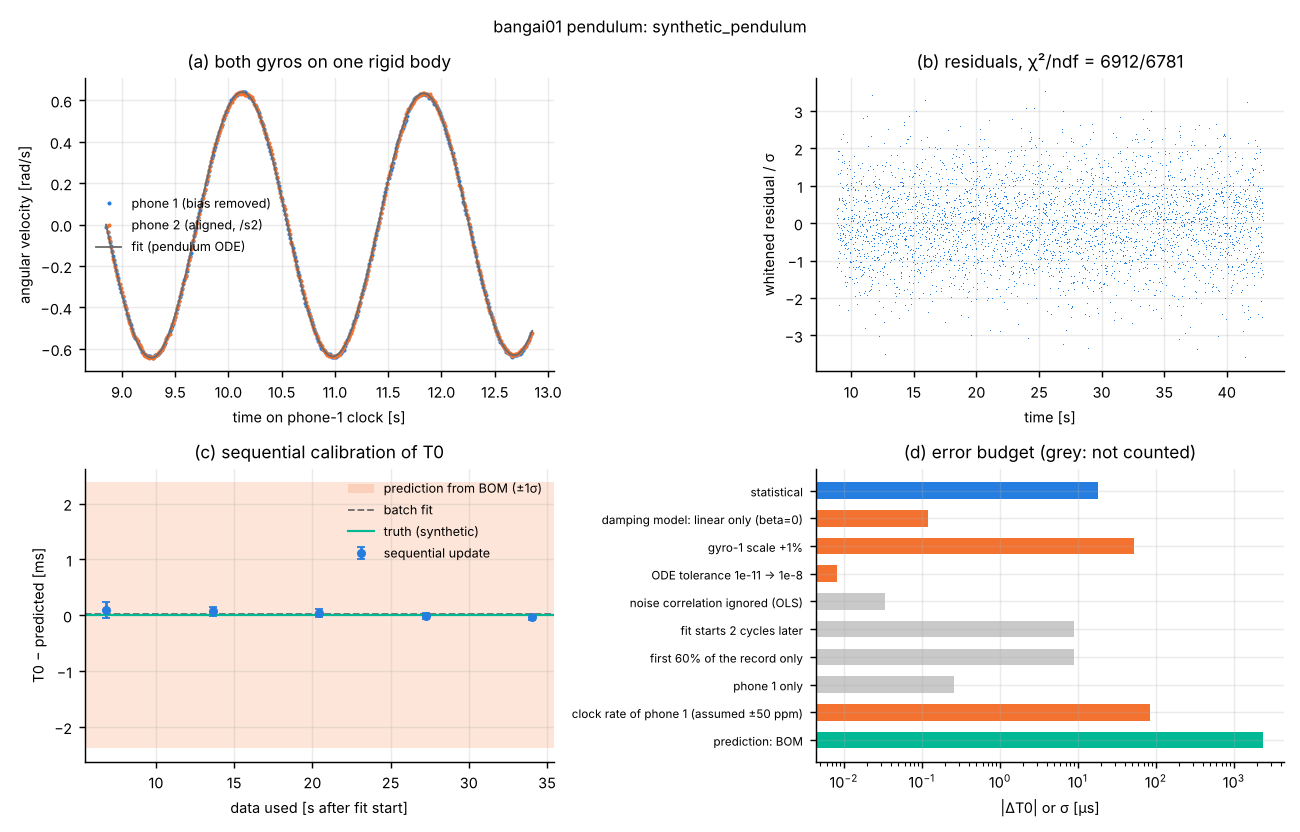
\includegraphics[width=0.92\textwidth]{bangai/bangai01_synthetic_pendulum.png}
\caption{実験 A の解析を合成データにかけた例。(a) 1 つの剛体として当てはめた 2 台のジャイロ、(b) 白色化した残差、(c) 逐次更新による $T_0$ の推定（橙の帯は部品表からの予測の ±1σ）、(d) 誤差の内訳（灰色は数えない項目）。予測の誤差（緑）が測定の誤差より 1 桁以上大きい。}\label{fig:bgpend}
\end{figure*}

\begin{figure*}[t]\centering
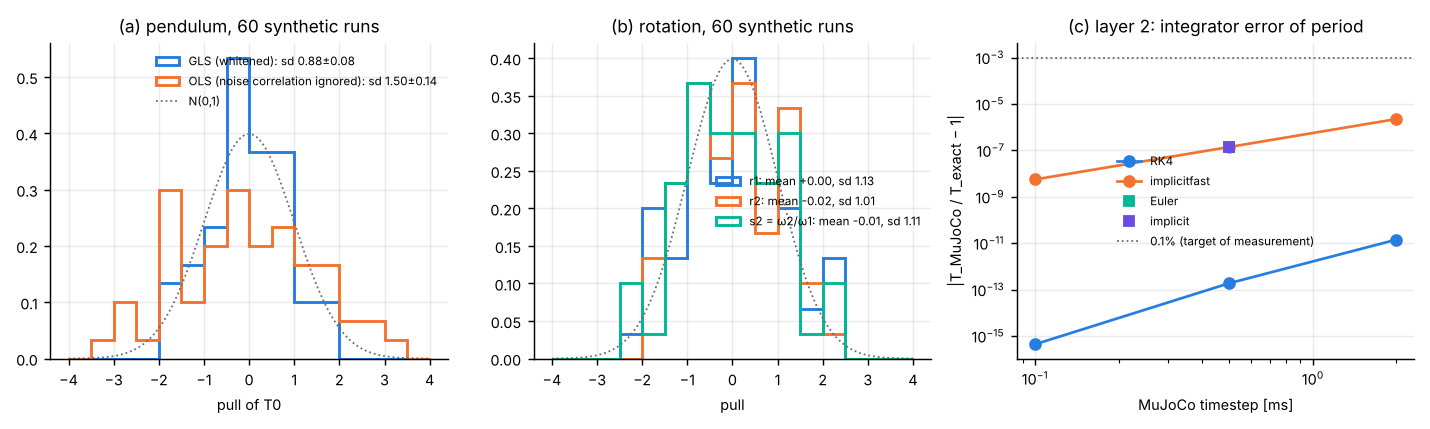
\includegraphics[width=0.98\textwidth]{bangai/bangai01_toys.png}
\caption{(a) 振り子の $T_0$ の pull（60 回）。雑音の相関を無視すると幅 1.50 で誤差を過小評価する。(b) 回転の pull（60 回）。(c) 2 層目：MuJoCo の周期の誤差と時間刻み。RK4 も implicitfast も測定の目標（0.1\%、点線）より桁違いに小さい。}\label{fig:bgtoys}
\end{figure*}

\subsection{残っていること}

\begin{itemize}\setlength{\itemsep}{0pt}
\item 実物の雑音が AR(1) で表せるかは、実測の静止区間の自己相関で確かめる。
\item 合成データの例 1 つで、$\tau_2$ の pull $-2.0$、$\kappa_2 = +46\pm10$ ppm（正解 20 ppm）。toy MC では $\tau_2$ の偏りは見えない（$+0.19\pm0.11$）ので 1 例の揺らぎと考えるが、$\kappa$ と $\tau$ の相関を含めて実測で確かめる。
\item $r_2/r_1$ の pull の幅 1.22。回転の 1 例で $r_2$ の pull +3.0。傾きの模型の位相を 1 台目のジャイロの積分で近似していることが疑わしい。
\item 回転の $\chi^2/\mathrm{ndf}=0.92$（自由度は実効的なパラメータの数 586 で数えた）。1 を下回る理由は未確認。
\item 零点の方法の偏り（$-0.58\sigma$）の原因の確認。
\end{itemize}
その先には、回転椅子に座って棒を手足の代わりに振り、胸に付けた端末で胴体の向きを記録して、式~(\ref{eq:ambac}) とループ 1 周の幾何学的位相を実物で確かめる実験を考えている。
椅子の軸の摩擦は、第~\ref{sec:upperground} 節の「足元の摩擦の境目」に当たる。


\part*{結び}
\addcontentsline{toc}{part}{結び}

\section{考察}\label{sec:discuss}

\textbf{安価なシミュレーションに答えられること}：
本稿の課題で、シミュレーションは「実機の挙動の予測」ではなく、
\textbf{(1) 学習に与えるべき構造、(2) 学習と制御の分担、(3) 組み合わせた形で効く仕組みと校正値、(4) 校正の試験動作と測るべき量とその誤差}を決めるために使われた。
いずれも、答えの分かっている試験台があるから判断できた。
大規模な GPU シミュレーションとドメインランダム化が「誤差の範囲を広く覆う」方向だとすると、本稿の方向は「どこに誤差があり、何を測ればよいか」を絞る方向であり、両者は補完的になりうる。ただし、これは本稿の事例に基づく仮説であり、両者を同じ課題で比べた検証は行っていない。

\textbf{誤差評価の手順が差を生む}：第~\ref{sec:fail} 節の失敗の多くは、計算資源ではなく評価の手順に由来した。
答えの分かっている照合、原因を 1 つずつ変える切り分け、多数回の試行による pull の確認、独立な標本どうしの比較は、いずれも CPU だけで実行でき、
しかも「誤差約 2\%」の正体（シミュレータの積分法）や、ばらつきの過小評価（F4・F13・F18）を明らかにした。
第~\ref{sec:bangai} 節では同じ手順を実物の実験の前に使い、予測の精度を決めるのが端末の重心であること、雑音の相関を無視すると誤差を 1.5 分の 1 に過小評価することを、測定の前に見つけた。
資源の限られた立場では、\textbf{計算の量ではなく評価の厳密さで、結果の信頼性を上げる}ことが現実的な戦略になる。

\textbf{一般化の射程}：第~\ref{sec:learn} 節の失敗の原因（正味の効果が入力の 2 次、すなわちリー括弧から生じる）は AMBAC に固有ではなく、
車両の縦列駐車に代表される非ホロノミック系、自由浮遊宇宙ロボット \cite{nakamura1991}、ヘビ型・遊泳型の移動など、形状の周期運動で全体を動かす系に共通する。
これらの系では正弦波入力による操舵 \cite{murray1993} が古典的な解法であり、振動子の構造が有効だったことと整合する。
したがって「構造なしの探索は 2 次の効果の前で停滞し、周期運動の構造で解消する」という仮説は、この系の族に対して検証可能な形で立てられる。
第~\ref{sec:calib} 節の「推定しにくい方向で数値誤差が拡大され、$\chi^2$ に現れない」という構造も、パラメータの一部の組み合わせしか観測できない同定問題一般に現れうる。
逆に、第~\ref{sec:bangai} 節の振り子のように測る量が推定しにくい方向に乗らなければ、同じシミュレータの積分法の誤差は $10^{-7}$ 以下で無視できる。シミュレータの数値誤差が効くかどうかは、シミュレータではなく\textbf{測る量と系の構造}で決まる。
一方、接触の細部、アクチュエータの非線形、柔軟体のように、誤差の主因がモデルの外にある課題には、本稿の枠組みは直接は届かない。

\textbf{答えられないこと}：PC の上だけでは sim-to-real ギャップそのものは確かめられない。
仮想の実機で絞り込めるのは、モデルに含めたパラメータについて、推定しやすい方向・しにくい方向と、手順上の落とし穴までである。
モデルに入れていない現象（接触の細部、モーターの非線形、部品のたわみ）は再現されず、誤差の見積もりにも現れない（F20 の端末の重心はその小さな例である）。\textbf{実機で初めて効いてくる未知の誤差源の優先順位は決められない}。
第~\ref{sec:upperground} 節のアクチュエータ・MR 流体・熱の数値は仮定の部品の値に基づき、流体ブレーキは速さとトルクの関係を式で与えた理想化したモデルである。

\textbf{上半身と下半身の検証の厚さ}：上半身は、式のモデル（Sim07・08）から MuJoCo の段階 12〜17 まで、仕組みを 1 つずつ足して同じ物差しで比べられた。
下半身は、第 3 版まで式のモデル（Sim09・10）が中心だったが、第 4・5 版で段階 18〜26（脚の円錐、足裏、段差、歩行、状態推定）を加え、上半身と同じ物差し（1 層目の予測と 2 層目の MuJoCo、誤差の 3 分類、失敗の記録）で比べられるようになった。
それでも、段階 9 は Sim09 の「静止しても転倒」の判定の意味（安全余裕 2 cm を差し引いた判定）を正確にし、2 層目の照合が 1 層目の結論を細かくすることを示した。
歩行では、計画は構造（LIPM・ZMP・capture point）を与えた手法に限り、学習は使っていない。成功の領域が島に分かれること（F37）は、構造なしの探索がさらに難しくなる場面であることを示しており、第~\ref{sec:learn} 節の仮説を学習で試すことは今後の課題である。

\textbf{学習手法の限定}：本稿の学習はすべて ES による。構造を与える効果が ES に特有のものか、PPO や SAC などの勾配に基づく強化学習を含むモデルフリー学習一般に成り立つかは、本稿の結果からは判断できない。
勾配に基づく手法では探索の初期の方策のばらつきが異なるため、2 次の効果による停滞の程度も変わりうる。同じ試験台で複数の学習法を比べることが、本稿の主張を強めるための最優先の課題である。


\section{今後の目標}

\begin{enumerate}\setlength{\itemsep}{0pt}
\item \textbf{3 層目の照合}：端末の重心を測ってから第~\ref{sec:bangai} 節の剛体と IMU の実験を行い、シミュレータの剛体の仮定と IMU の校正値を実物で確かめる。実験 B は 2 台の位置を入れ替えた記録を加え、目盛りの誤差を比で打ち消す。その後、安価なサーボのアーム 1 台で、仮想の実機で設計した校正手順を確認する。
\item \textbf{拘束条件つきの当てはめの拡張}：サーボの遅れ・摩擦の校正値を加えて地上の機体（段階 12〜17）へ広げ、総質量の計量や関節トルクのように推定しにくい方向を外から決める情報を拘束として加えて、$\chi^2$ で系統誤差を検出できるかを試す。
投球のような「速度差のある運動の連鎖」を、段ごとの拘束条件の連鎖として当てはめる（粒子の崩壊の連鎖の当てはめとの対応）ことも検討する。
\item \textbf{下半身の検証}：足の置き場所の MPC、立っている足の滑りの検出、3 次元の段差、大型の歩き方（第~\ref{sec:lowerrem} 節）。物理デバイスでは、足裏の力センサ・エンコーダ・IMU から重心を推定する構成（段階 25・26）を最初に試す。
\item \textbf{学習法と系の一般化}：同じ試験台での PPO・SAC との比較と、他の非ホロノミック系（正弦波操舵の古典例など）での構造仮説の検証。
\item \textbf{ハイブリッド制御}：計画を最適制御、実行時の補正を学習方策が担う制御の実装。
\item \textbf{誰でも使えるシミュレータへ}：部品表から機体を組み立て、性能表と校正データを CSV・JSON で書き出すまでをまとめてパッケージとして公開し、校正データを公開して機械学習による推定と物理モデルによる推定を同じデータで比べられるようにする。
\end{enumerate}


\section{まとめ}

実機も高精細なシミュレータも持たない条件で、CPU だけで動く安価なシミュレーションがフィジカル AI の課題にどこまで答えられるかを、AMBAC を試験台に検討した。
構造のない学習の失敗を物理の 2 次の効果として説明し、振動子の構造を与えた学習が理論上界の 98\% に達すること、
モデル誤差の下では学習が頑健だが保存量の計画は最適制御が担うべきこと、
部品表から組み立てた機体の試験で、止めるときの反作用・足元の摩擦の境目・荷重分布・サーボの遅れが性能を左右する校正値になること、
上半身では肩のひねりも幾何学的位相であり、動かす部品と止める部品を分けると速さと安全が両立すること、
下半身では宇宙で脚が最も効く肢である一方、地上の二本脚を支えるのは動かせる重い上体で、段差での脚の利点は人間大に限られること、歩行では腕の振りが足裏のねじれを打ち消す地上の AMBAC であり、実機で測れる量からの重心の推定と脚のオドメトリで安定化が働くこと、
答えを隠した仮想の実機で、校正の誤差を統計・計算・系統に分けて評価し、拘束条件つきの当てはめで推定ごとの誤差を正しく見積もれること、
ただし仮想の実機自身の数値誤差が系統誤差の源になり、それは当てはまりの良さに現れないことを示した。
実物との照合の最小の実験について、実物の前に解析を作って合成データで pull を確かめ、比較の精度を決めるのは測定ではなく部品表の予測（端末の重心）であることを示した。
さらに、うまくいかなかった 52 の試みを先行研究の既知の失敗と対応づけ、その多くが計算資源ではなく評価の手順に由来することを示した。
いずれも ES を用いた単一の系（歩行は構造を与えた計画）での事例であり、歩行は平らな床のシミュレーションに限る。一般化と実物での確認は今後の検証による。
安価なシミュレーションは実機の代わりではなく、\textbf{実機に何を持ち込むべきかを決める道具}として、計算資源の限られた研究者にも開かれている。

\appendix
\section{再現の手順と対応するファイル}
\small
すべてリポジトリ\footnote{\url{\repo}} の相対パスである。画面のない環境では \texttt{MUJOCO\_GL=disable} で実行する。
\begin{itemize}\setlength{\itemsep}{0pt}
\item 第~\ref{sec:learn}・\ref{sec:robust} 節：\texttt{sims/sim05*.py}（学習と制御の比較）。詳しい記録は \texttt{docs/05\_physical\_ai.md}。
\item 第~\ref{sec:field}・\ref{sec:fieldres} 節と第 II・III 部の段階：\texttt{sims/field*.py}（段階 1〜24）、図は \texttt{figures/field/}。記録は \texttt{docs/11}・\texttt{docs/12}・\texttt{docs/14}（下半身の段階 18〜24）。
\item 第 II 部の式のモデル：\texttt{sims/sim07\_spatial.py}・\texttt{sims/sim08\_shoulder.py}（記録は \texttt{docs/07}・\texttt{docs/08}）。第 III 部：\texttt{sims/sim09\_legs.py}・\texttt{sims/sim10\_steps.py}（\texttt{docs/09}・\texttt{docs/10}）。
\item 第~\ref{sec:calib} 節：\texttt{sims/field04b\_error\_budget.py}（誤差の内訳）、\texttt{sims/field04c\_kinfit.py}（kinematic fit、4 並列で約 30 分）、
\texttt{sims/field04d\_dispersion\_pool.py}（本版の再評価、既存の出力の再解析で数秒）。数値は \texttt{data/field04b\_summary.txt}、\texttt{data/field04c\_summary.txt}、\texttt{data/field04d\_summary.txt}。
\item 第~\ref{sec:fail} 節：\texttt{docs/13\_error\_evaluation\_kinfit.md} の 13.5 節。
\item 第~\ref{sec:bangai} 節：\texttt{sims/bangai01\_bar\_imu.py all}（合成データの作成・解析・toy MC、約 8 分）。数値は \texttt{data/bangai01\_summary.txt}、図は \texttt{figures/bangai/}、記録は \texttt{docs/13} の 13.7 節。実測は \texttt{analyze data/bangai01/<名前>/config.json} で同じ解析にかける（置き方は \texttt{data/bangai01/README.md}）。解説記事の原稿は \texttt{articles/ambac-bangai-bar-iphone-imu.md}（測定値は空欄）。
\end{itemize}

\section{改版の記録}
\small
\begin{description}\setlength{\itemsep}{0pt}
\item[第 1 版（2026-11-26）] 学術論文版レター \cite{letter2026} を土台に作成。
第 2 段階のシミュレーション場の方法と 17 段階の結果（第 5・6 節）、校正の誤差評価の全体と kinematic fit の表（第 7 節）、
失敗の記録（第 8 節、docs/13 §13.5 の F1〜F12 と段階ごとの索引に、本版の再評価で見つけた F13 を追加）、3 層目の照合の実験計画（第 9 節）を加えた。
レターの (b$'$) の 1 試行のばらつき「1.2〜1.4\%」を、独立な 2 標本 100 回の「1.37 / 1.45 / 1.63\%」に訂正し、kinematic fit による改善「約 3 割」を同じ試行での対応のある比較（0.70、95\% 区間 0.57〜0.87）として示し直した。
同時期に、内容を一般の技術者向けに書き直した解説記事（日本語・英語）の原稿をリポジトリの \texttt{articles/}・\texttt{books/}・\texttt{docs/Dev\_Comminuty/} に用意した（未公開）。
\item[第 2 版（2026-11-26）] 第 9 節を、計画から「実物の前に作った解析と、その合成データによる検証」に書き直した（\texttt{sims/bangai01\_bar\_imu.py}）。部品表からの予測とその誤差の内訳、MuJoCo の組み立てと積分法の確認、誤差の内訳（統計・系統・計算）、toy MC による pull の検定を加えた。第 1 版の誤差の見積もり（表）は端末の重心のずれを含まず、零点の方法の統計誤差も粗く見積もっていたので、合成データの値に置き換えた（F20）。失敗の記録に F14〜F20 を加え、分類を 4 つにした。実験そのものはまだ行っていない。
\item[第 3 版（2026-11-26）] 全体を 4 部構成（導入と全身の簡易シミュレーション／上半身の詳細／下半身の詳細／共通の土台）に組み替えた。
第 II 部（3 次元の肩とひねりの幾何学的位相、地上の腕の反作用・止め方・機能の分担、段階 17 の表）と第 III 部（宇宙の脚、二本脚と腰、段差と大きさ、下半身で残っている課題）を、第 1 段階の Sim07〜10 とシミュレーション場の段階 6・8〜10・12〜17 から新しく書いた。
第 2 版のシミュレーション場の結果の節のうち、地上の反作用と機能の分担は第 II 部へ移した。節の参照を番号の手書きから自動の参照に変えた。結果の数値は第 2 版から変えていない。
\item[第 4 版（2026-11-27）] 第 III 部に、下半身の MuJoCo での検証（段階 18〜24）を加えた：宇宙の脚の円錐の照合と可動域・干渉（段階 18）、足裏の摩擦と足首（段階 19）、二本脚の段差（段階 20）、歩行（第~\ref{sec:walk} 節：ZMP の計画、腕の振り、安定化、踏み出し）。
「下半身で残っている課題」を、確かめたことと残ることに書き直した。失敗の記録に F21〜F45 と、その分類を加えた。第 3 版までの数値は変えていない。
\item[第 5 版（2026-11-27）] 歩行の節（第~\ref{sec:walk} 節）に、実機で測れる量からの重心の推定（段階 25）と脚のオドメトリ（段階 26）、図~\ref{fig:lower3} を加えた。失敗の記録に F46〜F52 と分類「推定と制御の結合」を加えた。第 4 版で古いまま残っていた「まとめ」（失敗の数、歩行を扱っていない）と「今後の目標」の下半身の項を直した。第 4 版までの数値は変えていない。
\end{description}

\begin{thebibliography}{99}\footnotesize\setlength{\itemsep}{0pt}
\bibitem{letter2026} simulation\_AMBAC プロジェクト, 「安価なシミュレーションと校正値はフィジカル AI の何を助けるか --- 手足による姿勢制御（AMBAC）を『答えの分かっている試験台』として ---」, 学術論文版（レター）, 2026（\texttt{report/letter/letter\_formal.tex}）.
\bibitem{tobin2017} J.~Tobin et al., ``Domain randomization for transferring deep neural networks from simulation to the real world,'' \textit{IROS}, 2017.
\bibitem{peng2018} X.~B.~Peng, M.~Andrychowicz, W.~Zaremba, P.~Abbeel, ``Sim-to-real transfer of robotic control with dynamics randomization,'' \textit{ICRA}, 2018.
\bibitem{hwangbo2019} J.~Hwangbo et al., ``Learning agile and dynamic motor skills for legged robots,'' \textit{Science Robotics}, 4(26), 2019.
\bibitem{ijspeert2008} A.~J.~Ijspeert, ``Central pattern generators for locomotion control in animals and robots: a review,'' \textit{Neural Networks}, 21(4), 642--653, 2008.
\bibitem{iscen2018} A.~Iscen et al., ``Policies modulating trajectory generators,'' \textit{CoRL}, PMLR 87, 916--926, 2018.
\bibitem{atkeson1986} C.~G.~Atkeson, C.~H.~An, J.~M.~Hollerbach, ``Estimation of inertial parameters of manipulator loads and links,'' \textit{IJRR}, 5(3), 101--119, 1986.
\bibitem{gautier1990} M.~Gautier, W.~Khalil, ``Direct calculation of minimum set of inertial parameters of serial robots,'' \textit{IEEE Trans. Robotics and Automation}, 6(3), 368--373, 1990.
\bibitem{makoviychuk2021} V.~Makoviychuk et al., ``Isaac Gym: High performance GPU-based physics simulation for robot learning,'' \textit{NeurIPS Datasets and Benchmarks}, 2021.
\bibitem{kane1970} T.~R.~Kane, M.~P.~Scher, ``Human self-rotation by means of limb movements,'' \textit{J. Biomechanics}, 3(1), 39--49, 1970.
\bibitem{kane1969} T.~R.~Kane, M.~P.~Scher, ``A dynamical explanation of the falling cat phenomenon,'' \textit{Int. J. Solids and Structures}, 5(7), 663--670, 1969.
\bibitem{montgomery1993} R.~Montgomery, ``Gauge theory of the falling cat,'' in \textit{Dynamics and Control of Mechanical Systems}, Fields Inst. Commun. 1, AMS, 1993.
\bibitem{marsden1992} J.~E.~Marsden, \textit{Lectures on Mechanics}, Cambridge University Press, 1992.
\bibitem{brockett1983} R.~W.~Brockett, ``Asymptotic stability and feedback stabilization,'' in \textit{Differential Geometric Control Theory}, Birkhäuser, 181--191, 1983.
\bibitem{salimans2017} T.~Salimans et al., ``Evolution strategies as a scalable alternative to reinforcement learning,'' arXiv:1703.03864, 2017.
\bibitem{todorov2012} E.~Todorov, T.~Erez, Y.~Tassa, ``MuJoCo: A physics engine for model-based control,'' \textit{IROS}, 2012.
\bibitem{nakamura1991} Y.~Nakamura, R.~Mukherjee, ``Nonholonomic path planning of space robots via a bidirectional approach,'' \textit{IEEE Trans. Robotics and Automation}, 7(4), 500--514, 1991.
\bibitem{murray1993} R.~M.~Murray, S.~S.~Sastry, ``Nonholonomic motion planning: steering using sinusoids,'' \textit{IEEE Trans. Automatic Control}, 38(5), 700--716, 1993.
\bibitem{avery1998} P.~Avery, ``Applied fitting theory VI: Formulas for kinematic fitting,'' CLEO Note CBX 98-37, 1998.
\bibitem{fruhwirth1987} R.~Frühwirth, ``Application of Kalman filtering to track and vertex fitting,'' \textit{Nucl. Instrum. Methods A}, 262, 444--450, 1987.
\bibitem{johannink2019} T.~Johannink et al., ``Residual reinforcement learning for robot control,'' \textit{ICRA}, 2019.
\bibitem{barlow2002} R.~Barlow, ``Systematic errors: facts and fictions,'' arXiv:hep-ex/0207026, 2002.
\bibitem{neyman1948} J.~Neyman, E.~L.~Scott, ``Consistent estimates based on partially consistent observations,'' \textit{Econometrica}, 16(1), 1--32, 1948.
\bibitem{codman1934} E.~A.~Codman, \textit{The Shoulder}, Thomas Todd, Boston, 1934.
\bibitem{horak1986} F.~B.~Horak, L.~M.~Nashner, ``Central programming of postural movements: adaptation to altered support-surface configurations,'' \textit{J. Neurophysiology}, 55(6), 1369--1381, 1986.
\bibitem{phyphox} S.~Staacks, S.~Hütz, H.~Heinke, C.~Stampfer, ``Advanced tools for smartphone-based experiments: phyphox,'' \textit{Physics Education}, 53(4), 045009, 2018.
\bibitem{kajita2003} S.~Kajita et al., ``Biped walking pattern generation by using preview control of zero-moment point,'' \textit{ICRA}, 1620--1626, 2003.
\bibitem{pratt2006} J.~Pratt, J.~Carff, S.~Drakunov, A.~Goswami, ``Capture point: A step toward humanoid push recovery,'' \textit{IEEE-RAS Humanoids}, 2006.
\bibitem{englsberger2015} J.~Englsberger, C.~Ott, A.~Albu-Sch\"affer, ``Three-dimensional bipedal walking control based on divergent component of motion,'' \textit{IEEE Trans. Robotics}, 31(2), 355--368, 2015.
\bibitem{collins2009} S.~H.~Collins, P.~G.~Adamczyk, A.~D.~Kuo, ``Dynamic arm swinging in human walking,'' \textit{Proc. R. Soc. B}, 276, 3679--3688, 2009.
\end{thebibliography}

\end{document}
